

\documentclass[12pt,letterpaper]{article}

\usepackage{setspace}
%\doublespacing
\linespread{1.25}
%\linespread{2}
\usepackage{geometry}

\geometry{letterpaper, margin=1in}
%\usepackage{times}
\usepackage{pslatex}
\usepackage{apacite}
\usepackage{url}
\usepackage{graphicx}
\usepackage{caption}
\usepackage{subcaption}
\usepackage{listings}
\usepackage{color}
\usepackage{textcomp}
\usepackage{amsmath}
\usepackage{amssymb}
\usepackage{wrapfig}
\usepackage{lipsum}
\usepackage{setspace}
\usepackage{booktabs}

\usepackage{fancyhdr}
\pagestyle{fancy}
\renewcommand{\headrulewidth}{0pt}
\fancyhf{}
\fancyhead[R]{\thepage}
\lhead{\textsc{pragmatic theory of generic language}}
 
\graphicspath{{../figures/}}
  \newcommand*\diff{\mathop{}\!\mathrm{d}}

\def\signed #1{{\leavevmode\unskip\nobreak\hfil\penalty50\hskip2em
  \hbox{}\nobreak\hfil(#1)%
  \parfillskip=0pt \finalhyphendemerits=0 \endgraf}}

\newsavebox\mybox
\newenvironment{aquote}[1]
  {\savebox\mybox{#1}\begin{quote}}
  {\signed{\usebox\mybox}\end{quote}}


 \newcommand{\denote}[1]{\mbox{ $[\![ #1 ]\!]$}}

\definecolor{Red}{RGB}{255,0,0}
\newcommand{\red}[1]{\textcolor{Red}{#1}}  
\definecolor{Green}{RGB}{10,200,100}
\definecolor{Blue}{RGB}{10,100,200}
\newcommand{\ndg}[1]{\textcolor{Green}{[ndg: #1]}}  
\newcommand{\mht}[1]{\textcolor{Blue}{[mht: #1]}}  

\usepackage{titlesec}

\setcounter{secnumdepth}{4}

\titleformat{\paragraph}
{\normalfont\normalsize\bfseries}{\theparagraph}{1em}{}
\titlespacing*{\paragraph}
{0pt}{3.25ex plus 1ex minus .2ex}{1.5ex plus .2ex}

\title{A pragmatic theory of generic language}
%\title{Generics are vague: A formal theory of generalizations in language}
%\title{Generics are vague: a probabilistic model of generic language}
%\title{Generic language is vague yet rationally understood}
%\title{Generic language is vague yet pragmatically understood}
%\title{Generic language is vague yet pragmatically used}

\author{{\large \bf Michael Henry Tessler} (mtessler@stanford.edu)\\ {\large \bf Noah D. Goodman} (ngoodman@stanford.edu) \\
  Department of Psychology, Stanford University}
  
 \date{}
\begin{document}

\maketitle

%A Pragmatic Theory of Generic Language 

Running head: \textsc{pragmatic theory of generic language}

\vspace{80 mm}
{\setstretch{1.0}
\textsc{\\corresponding author \\
Michael Henry Tessler \\
Stanford University, Department of Psychology \\
450 Serra Mall, Bldg. 420, Rm. 316 \\
Stanford, CA 94305 \\
mtessler@stanford.edu \\
757 - 561- 7071}

}
\newpage
%\contributor{Submitted to Proceedings of the National Academy of Sciences
%of the United States of America}

%%%Newly updated.
%%% If significance statement need, then can use the below command otherwise just delete it.

%
%\significancetext{
%Understanding the world requires making generalizations about categories; we use generic language to convey such generalizations: `dogs bark', `rats carry disease', and `liberals drink lattes'.
%These simple sentences are common in ordinary conversation, child-directed speech, and political discourse.
%They are how we teach, how we motivate, and how we persuade (or mislead) others.
%Yet the precise meaning of generics is a puzzle that has resisted formalization.
%We introduce a mathematical model of generic language by combining principles of language understanding with a basic meaning in terms of property statistics.
%This theory provides the connective tissue between generic language and conceptual knowledge and gives insight into how everyday language use is tied to beliefs. 


%of the parties involved.
%
%Understanding the world requires making generalizations about categories.
%Generic language (e.g. \emph{Dogs bark.}) provides an efficient and ubiquitous way to transmit this kind of information.
%Yet, these common, simple sentences that even 2-year-olds can comprehend have philosophically puzzling qualities which have impeded precise formalization. 
%We explain the apparent paradoxes using a meaning of generic language that is simple but underspecified. 
%With uncertainty in the language, general principles of communication and 
%interlocutors' shared beliefs about the categories and properties in question 
%are responsible for establishing a precise meaning in context.
%This theory provides the connective tissue between generic language and conceptual knowledge and demonstrates 
% how beliefs play a foundational role in understanding language. 
 %
 % We find this model to explain almost all of the variance in human judgments of the acceptability of familiar generic sentences and 
% to human interpretations of unfamiliar generic sentences.
%to others forms the fabric of conceptual developmental and cultural transmission.
%Utterances that convey generalizations----generic utterances----are ubiquitous in everyday conversational and child-directed speech, 
%yet there is to date no formal account of their precise meanings.
%Humans build internal representations of the world by making generalizations about categories, and use language to convey these generalizations to 
%M.H.T. and N.D.G developed theory and designed research; M.H.T. performed research and analyzed data. M.H.T. and N.D.G. wrote the paper.
%}

%\maketitle

\begin{abstract}
{Generalizations about categories are central to human understanding, and generic language (e.g.~\emph{Dogs bark.}) provides a simple and ubiquitous way to communicate these generalizations. 
Yet the meaning of generic language is philosophically puzzling and has resisted precise formalization.
We explore the idea that the core meaning of a generic sentence is simple but underspecified, 
and that general principles of pragmatic reasoning are responsible for establishing the precise meaning in context.
Building on recent probabilistic models of language understanding, we provide a formal model for the evaluation and comprehension of generic sentences. 
This model explains the puzzling flexibility in usage of generics in terms of diverse prior beliefs about properties.
We elicit these priors experimentally and show that the resulting model predictions explain almost all of the variance in human judgments for both common and novel generics.
This theory provides the mathematical bridge between the words we use and the concepts they describe.
}
\end{abstract}

\newpage
%\keywords{generic language | semantics | pragmatics | categories}

Most would agree that \emph{Swans are white}, but certainly not every swan is.
This type of utterance conveys a generalization about a category (i.e. \textsc{swans}) and is known as a generic utterance \cite{Carlson1977,Leslie2008}.
Communicating generically about categories is useful because categories themselves are unobservable \cite{Markman1989}.
%Knowledge about categories, while central to human reasoning, is tricky to acquire because categories themselves are unobservable \cite{Markman1989}.
It is believed that every language can express generic meaning \cite{Behrens2005,Carlson1995}, and that generics are essential to the growth of conceptual knowledge \cite{Gelman2004} and how kinds are represented in the mind \cite{Leslie2008}.
Generic language is ubiquitous in everyday conversation as well as in child-directed speech \cite{Gelman2008}, and children as young as two or three understand that generics refer to categories and support generalization \cite{Cimpian2008}.
% and though English and many other languages do not possess an unambiguous form devoted to generic meaning \cite{Behrens2000, AlMalki2014}. 
Additionally, generics are the primary way by which speakers discuss social categories, making them key to propagating stereotypes \cite{GelmanEtAl2004,Rhodes2012,Leslie2015} and impacting motivation \cite{Cimpian2010motivation}.
Despite their psychological centrality, apparent simplicity, and ubiquity, a formal account of generic meaning remains elusive.

The major issue in formalizing generic language is determining what makes a generic sentence true or false.
At first glance, generics feel like universally-quantified statements as in \emph{all swans are white}. 
Unlike universals, however, generics are resilient to counter-examples (e.g., \emph{swans are white} even though there are black swans). 
Intuitions fall back to something more vague like \emph{swans, in general, are white} because indeed most swans are white.
But mosquitos, in general, do not carry malaria, yet everyone agrees \emph{mosquitos carry malaria}.
%Interpreting the generic as meaning ``most'' (i.e. \emph{Most swans are white}) captures many cases, but cannot explain why \emph{Robins lay eggs} and \emph{Mosquitos carry malaria} are so intuitively compelling: Only adult female robins lay eggs and a very tiny fraction of mosquitos actually carry malaria.
Indeed, it appears that any \emph{truth condition} stated in terms of how common the property is within the kind violates intuitions.
Consider the birds: for a bird, being female practically implies you will lay eggs (the properties are present in the same proportion), yet we say things like \emph{birds lay eggs} and we do not say things like \emph{birds are female}.

% as , even though the two properties are present in the same proportion (about 50\%) in the category of robins.
%\ndg{No precise meaning formalized in the mathematical language of logic seems to be sufficient to capture the meaning of natural language generics.}

%Generics are additionally puzzling in how they are interpreted. 
%The mystery deepens with how generic language is interpreted.
How particular interpretations arise from generic language is also a mystery.
%The strong interpretation of novel generics deepens the mystery.
The case of \emph{mosquitos carry malaria} suggests the generic must in some way be analogous to ``some'' (i.e. \emph{Some mosquitos carry malaria.}). 
Yet, the empirical literature suggests generics are often interpreted as implying the property is widespread:
There is a difference between \emph{some swans have hollow bones} and \emph{swans have hollow bones} \cite{Gelman2002}.
When interpretations are compared directly against \emph{truth conditions} (i.e., how prevalent a property would need to be for the generic to be true), both children and adults infer the property is more prevalent when told the generic than when judging the generic true \cite{Cimpian2010,Brandone2014}, suggesting that speakers who use generics can exaggerate evidence to their listener.
%Both children and adults believe the generic implies the property-in-question is even more widespread than when asked how common the property would need to be for the generic to apply

How can generics have such flexible truth conditions while simultaneously carrying strong implications?
In this paper, we explore the idea that the core meaning of a generic statement is simple, but underspecified, and that general principles of communication may be used to resolve precise meaning in context. 
In particular, we develop a mathematical model that describes pragmatic reasoning about the degree of prevalence required to assert the generic.  
We find that this formalism resolves the philosophical and empirical puzzles.

In Section 1, we review extant theories of generics from the linguistic and psychological literatures.
In Section 2, we describe our pragmatic theory of generic language in formal terms and illustrate the model through simulation. 
In Section 3, we conduct a set of experiments to test the \emph{truth conditions of generic statements}, and find our model predicts the patterns in human endorsement of familiar generic sentences.
We also find that the prior beliefs used in the Bayesian model reflect conceptual structure, and this provides an understanding of the conceptual implications of generics.
In Section 4, we conduct a set of experiments to test \emph{interpretations of novel generic sentences}, again finding our model predicts human judgments with high quantitative accuracy.
In Section 5, we investigate the underlying semantic scale in more detail, and find that the core meaning of generic language depends in a crucial way on subjective beliefs, not mere frequency.

%The model predicts the patterns in both human endorsement of familiar generic sentences and interpretation of novel generic sentences. 
%Finally, we investigate the underlying semantic scale in more detail, and find that the core meaning of generic language depends in a crucial way on subjective beliefs, not mere frequency.
%In addition, the theory elucidates the nature of generic language: It is language whose semantics depend fundamentally on beliefs.
%\ndg{possibly we should expand this paragraph to give a bit more of a roadmap of the paper? "in section X we..."}

\subsection*{The philosophical puzzle of generic language: Truth conditions}

Generics express a relation between a kind K (e.g., \textsc{robins}) and a property F (e.g., \textsc{lays eggs}), such that the property can also be said to be applicable of an individual (i.e., the bird in my backyard lays eggs).
%These are in contrast to properties only predicable of the kind as a whole (e.g., \emph{Dogs are widespread})\footnote{No particular instance of dog can itself be widespread.}.
Bare plural statements (e.g., \emph{Robins lay eggs}) tend strongly to yield a generic meaning \cite{Carlson1977}, though other forms can express such a meaning sometimes (e.g., \emph{A mongoose eats snakes.}).
%\ndg{the previous sentence is sort of out of context. cut it, move it, or work it in better...}

Given that generics express a property that can be applied to individuals, it would seem intuitive that the number of individuals with the property would be what makes the statement true or false.
Counter-examples like \emph{Mosquitos carry malaria} and \emph{Birds lay eggs} v. \emph{Birds are female} stifle such intuition. 
Semantic theories that appeal to the statistics of the world (i.e., how many Ks have F) try to rescue the notion that a generic expresses something like \emph{Ks, in general, have F}, where \emph{in general} is often either restricted to particular domains or is calculated with particular distortions.
Alternative, \emph{conceptually}-based theories take a generic to mean \emph{Ks, in virtue of being the kind of things that Ks are, have F}.
These accounts appeal to structured, conceptual representations in deciding what kinds of generic statements are true or false.
Statistical and conceptual theories express the major contrasting views of the truth conditions of generic statements \cite{Carlson1995essay}.\footnote{We use the terms statistical and conceptual to refer to what \citeA{Carlson1995essay} referred to as ``inductive'' and ``rules and regulations'' views, respectively.}


\subsubsection*{Statistical accounts of generics}

Statistical accounts take the \textbf{property prevalence} to be fundamental: \emph{Birds lay eggs} means \emph{Birds, in general, lay eggs}. 
Of course, birds do not in general lay eggs (it's only the adult, female ones that do).
The primary way of dealing with such issues is to posit domain restrictions (``implicitly, we are only talking about the females'') when there are ``salient partitions'' \cite{Carlson1995}.
%Not all accounts of generic language reduce to puzzles about mental representation of kind--property relations.
%Accounts stemming from formal semantics tend to look towards precise, quantifiable conditions to determine if a sentence is true or false.
The most fully-developed theory on this front is due to \citeA{Cohen1999}. %The most promising account of generics in this tradition was put forth by 
Let's first introduce some notation:

For a given kind $K$ (e.g.~\textsc{robins}) and property $F$ (e.g.~\textsc{lays eggs}), we refer to the probability that an instance of kind $K$ has property $F$, that is $P(F\mid K)$, as the \emph{prevalence} of $F$ within $K$.
Logical quantifiers can be described as conditions on prevalence (i.e.~\emph{some} is $P(F\mid K)>0$, \emph{all} is $P(F\mid K)=1$). 
Assuming the generic relates to the property prevalence, then the simplest meaning would similarly be a threshold on prevalence: $P(F\mid K)>\theta$. \citeA{Cohen1999} takes $\theta = 0.5$; that is, \emph{Robins lay eggs} is roughly taken to mean \emph{More than half of (relevant) robins lay eggs}. 

Cohen introduces constraints into the computation of prevalence: $P(F\mid K)$. In particular, prevalence is computed with respect to a \emph{partition set}. 
The property \emph{lays eggs} induces a set of alternatives that all have to do with procreation (e.g. \emph{gives birth to live young}, \emph{undergoes mitosis}, ...).
The individuals that enter into the prevalence computation are only those individuals that would satisfy one or another alternative. 
That is, the only individuals under consideration are the female members of kinds because only the female members can plausibly satisfy one or another of the alternatives.
The inference that this sort of domain restriction is applied, as well as other constraints posited in the theory, are thought to be a pragmatic inference, though specifying the details of the pragmatics is beyond the scope of Cohen's theory.
Without a well specified theory of pragmatics, however, we have no general solution to map from property prevalence to truth judgment.
Conceptual information seems to be behind the pragmatic inference, but how Cohen's and other prevalence-based accounts relate to such knowledge remains obscure \cite{Carlson1995essay}.
\footnote{However, see \citeNP{Cohen2004} for a discussion of how his semantic constraints relate to different kinds of generics and different kinds of conceptual representational frameworks found in cognitive science.}

%Thus, \emph{Birds lay eggs} is roughly taken to mean \emph{Most female birds lay eggs}. 
%Further constraints are articulated with respect to time, so that incidental pertuba
%Further constraints are posited (e.g. further partitions with respect to time). 
%The constraints discussed 
%The theory, though mathematically rigorous and rationally appealing, relies upon a number of a working parts that need to be determined in some (unspecified) way by pragmatics. 
%In addition, it is unclear how to get from this semantic theory to the unspecified pragmatic theory on which it relies.



%Theories concerning the meaning of generic statements fall under two main headers: the statistical and the conceptual \cite{Carlson1995essay}.
%Statistical theories follow in the tradition of formal semantics, with an aim to provide a unified and quantitative set of conditions.
%Roughly speaking, statistical theories try to rescue the notion that \emph{swans, in general, are white} and articulate constraints on the computation of \emph{in general} in order to make it so.
%Others have looked beyond quantitative conditions and appeal to structured, conceptual representations.
%For these kinds of \emph{conceptual} theories, \emph{swans are white} means something like \emph{swans, in virtue of being the kind of thing that swans are, are white}.
%Not everybody wants to rescue a unified, formal mechanism of meaning 

%Semantic theories of generics aim to unify the diverse meanings associated with this simple, syntactic construction. 
%\citeA{Carlson1977} hints at what is necessary:
%%
%\begin{quote}
%What is suggested, then, is that the apparent variation in ... truth-conditions .. can be attributed to our \emph{strategies of investigation} and not to any inherent semantic marker in the sentence (in particular, a quantifier). [emphasis ours]
%\end{quote}
%%
%For \citeauthor{Carlson1977}, there are different \emph{strategies} to verify if a kind has a particular type of property 
%(e.g. to verify if a kind \emph{lays eggs} one can employ the strategy to consult only the female members of the kind). 
%Later accounts developed this argument to appeal to structured, conceptual representations (e.g. \emph{Bishops move diagonally} not because most bishops do but because the laws of chess mandate that they do). 
%These stand in contrast with semantic theories of generics that appeal to the statistics of the world (e.g. \emph{Barns are red} because most barns are; \citeNP{Carlson1995essay}).
%We review both classes of accounts below.

%(Incidentally, he argued that this was incompatible with the generic being analogous to a quantifier, a point we will dispute.)
%Since that time, there have been many other accounts of generics. 
%We follow \citeA{Carlson1995essay}, and organize the extant theoretical literature by theories that appeal to either the statistics of the world (e.g. \emph{Barns are red} because most barns are) or 
\subsubsection*{Conceptual accounts of generics}

Conceptual accounts of generics emphasize the structure of generic knowledge \cite{Prasada2000}, and view generic utterances as the way of expressing special mental relationships between kinds and properties \cite{Leslie2008, Prasada2012}.
\emph{Bishops move diagonally} because those are the rules of the game, not because they \emph{tend to} move diagonally.
How do we come to know the rules of the game, though?
\citeA{Leslie2007} introduces the notion that generics are tied to a ``default mode of generalization''. 
This ``default mode'' comes equipped with the ability to single-out \emph{striking properties} (e.g. properties which are dangerous or appalling) as particularly useful aspects of the world to know about. 
Hence, \emph{Mosquitos carry malaria} is true because it is a useful bit of information to convey.

Such an argument needs to be further augmented to capture inutitions: non-malaria carrying mosquitos must \emph{have the potential} to carry malaria, while other insects or animals must not. Otherwise, \emph{Insects carry malaria} or \emph{Animals carry malaria} would also be true \cite{Leslie2007}.
``Negative'' counter-instances must be distinguished from ``positive'' counter-instances: ``not having F'' (e.g. a bird that doesn't lay eggs) is not the same as ``having not-F'' (e.g. a hypothetical bird that bears live young).
When positive counter-instances exist, the generic is much less reasonable (e.g. \emph{Birds are female} seems weird because ``being male'' is a positive counter-instance of ``being female''). 
When only negative counters-instances exist, the generic is fine (e.g. \emph{Birds lay eggs.} since there no such bird that bears live young).
For properties that have no principled relationship to the kind (e.g., in \emph{Barns are red}), conceptual accounts fall back to statistical information: \emph{Ks, in general, have F}.

Empirical, psychological work supports this perspective.
\citeA{Prasada2006} distinguish between \emph{statistical} and \emph{principled relations} within concepts. 
These distinct relation types manifest themselves empirically as different inferences one could draw concerning the kind and property. 
For example, these include the expectation that the relation will hold for future instances (operationalized using the phrase \emph{In general, Ks have F}), the explanation that the relation holds because of the kind of thing that K is (\emph{Ks have F by virtue of being a K}), and that the principled relation is normative (\emph{Ks should have Fs}).
%These different kinds of relations relate to \citeA{Leslie2007}'s distinctions among generics.
\citeA{Prasada2013} found generics like \emph{Birds lay eggs} (in which only a minority of K have F) exhibit characteristics of principled connections, supporting \citeA{Leslie2007}'s typology.
Striking generics (e.g. \emph{Mosquitos carry malaria}) do not have the characteristics of principled connections, but do show characteristics of a third kind of connection: a \emph{causal connection} (operationalized using the phrase \emph{There is something about Ks that cause them to F}). 
Different kinds of kind--property relations exhibit qualitatively different kinds of connections. 
%This is taken to support \citeA{Leslie2007}'s typology of different types of default generalizations.

%The puzzles of generic language then reduce to puzzles about mental representation of kind-property relations.


%If this is the case, then a relatively simple semantic theory, phrased in terms of statistical regularities in the world, could be enough to formalize generic language.
%Abstract, mental representations may still operate; yet we suggest generic language operates through the common currency of probability. 

\ndg{ clean up this section to read less listy and more like a description of the essential ideas from this viewpoint, and highlights of empirical support (if that's relevant).}


\subsection*{The pragmatic perspective}

We find both the statistical and conceptual accounts compelling, but an important perspective is missing.
We note that generic language is not unique in its flexibility.
Understanding language in general depends upon assumptions interlocutors make about each other and what content is under discussion. 
The pragmatic lens reveals that utterances carry a mosaic of interpretations with a complex sensitivity to context \cite{Clark1996,Grice1975,Levinson2000}. 
Can the puzzles of generic language be understood as effects of pragmatic reasoning?
If so, we may be able to get away with a relatively simple, statistical,  semantic theory.
Abstract mental representations, then, may be the conceptual backdrop against which generic language is interpreted. 

We pursue such a line of inquiry, assuming the simplest truth-conditional meaning: a threshold on prevalence $P(F\mid K)>\theta$ (cf.\citeA{Cohen1999}).
%\footnote{Because we aim to explain the psycholinguistics of generics, we are generally interested in the subjective probability, not the actual frequency in the world.}
No fixed value of the threshold, $\theta$, would allow for the extreme flexibility generics exhibit (e.g. \emph{Mosquitos carry malaria}; \emph{Robins lay eggs} v. \emph{Robins are female}), % simultaneously with the interpretations of some novel generics being strong. 
so instead we allow this threshold to be established in context through pragmatic reasoning. % and is not a fixed property of the language.
Such an inference would depend on background knowledge about properties and categories---potentially structured, conceptual knowledge.
This inference, nonetheless, is a general mechanism of language not specific to interpreting generic statements.
We formalize this hypothesis in the Rational Speech Act (RSA) theory---a formal, probabilistic theory of language understanding.
RSA is derived from social reasoning, formalized as recursive Bayesian inference between speaker and listener \cite{Frank2012,Goodman2013,Goodman2016}. \ndg{last ref is the new tics review...}
Appendix A presents a brief tutorial on RSA for the reader unfamiliar.
% We will describe the basic RSA framework before articulating the full pragmatic theory of generic meaning.

%\subsubsection*{The pragmatic theory of generic meaning}

We follow the treatment of RSA applied to vague adjectives (e.g.~\emph{tall}), where a semantic variable is left underspecified \cite{Lassiter2013,Lassiter2015}.
We model the interpretation of generic statements by a pragmatic listener ($L_1$), concerned with learning the prevalence of a certain property in a certain category, $x=P(F \mid K)$.
She resolves the likely prevalence $x \in [0, 1]$ upon hearing a generic utterance $u$, by integrating her prior beliefs about $x$ with the generative process of the utterance -- an informative speaker ($S_1$).
%
\begin{eqnarray}
L_{1}(x , \theta \mid u) &\propto& S_{1}(u \mid x, \theta) \cdot P(x) \cdot P(\theta) \label{eq:L1}
\end{eqnarray}
%
%The pragmatic listener $L_1$ (Eq.~\ref{eq:L1}) is trying to resolve the value of $x$, how widespread F is within K (i.e.~$x = P(F\mid K) \in [0, 1]$) after hearing a generic utterance $u$. 
%Because the speaker's choice of utterance can depend on the prevalence threshold, $\theta$, used to establish the meaning of the generic, the 
%%The semantic variable $\theta$ (i.e. the threshold) underspecified in the lexicon. 
%That is, 
In addition to not knowing what $x$ is \emph{a priori}, the listener does not know the value of the prevalence threshold, $\theta$, used to establish the meaning of the generic (as described below). Because the speaker's choice of utterance can depend on the  threshold the listener must reason about this as well, based on her prior distribution over possible thresholds $P(\theta)$.
In principle, thresholds could be learned over time for different contexts, but here we assume the listener has no informative knowledge about the threshold: $\theta \sim \text{Uniform([0,1])}$.

To resolve an appropriate meaning, the listener uses her background knowledge about the property $P(x)$ and her intuitive theory of a speaker $S_1$ as a rational actor who has the goal of providing information to a hypothetical literal listener ($L_0$):
\begin{eqnarray}
S_{1}(u \mid x, \theta) &\propto& \exp{(\lambda_1 \cdot \ln  ( {L_{0}(x \mid u, \theta)} ) ) }\label{eq:S1}
\end{eqnarray}
%
%$L_1$ assumes  expresses something about how common the property is 
%(she knows it is a threshold on prevalence), 
%but doesn't know exactly what it conveys (she has uncertainty about the threshold.
The listener believes the speaker $S_1$ knows the threshold $\theta$.
That is, the speaker had a particular meaning in mind, and the listener can use pragmatic reasoning to help resolve that meaning \cite{Lassiter2013, Lassiter2015, GoodmanLassiter}. 

The proportionality in Eq.~\ref{eq:S1} implies normalization over a set of alternative utterances.
%Implicitly, there is a cost to producing an utterance $C(u)$, and this cost function is used to encode the alternative utterances the speaker could produce. 
%The speaker's prior distribution over utterances $P(u)$ encodes the alternative utterances the speaker could produce. 
We consider the simplest set of alternatives, including only the production of a generic utterance and the possibility of staying quiet (and we assume no difference in production cost between these alternatives). 
We adopt the simplest meaning of a generic utterance in terms of prevalence, a threshold function: $\denote{\text{K F}}(x, \theta)=x>\theta$.
The silent or \emph{null} utterance alternative carries no information (i.e.~$\denote{null}(x, \theta)=T$) and produces a posterior distribution in the listener identical with the prior.\footnote{
This alternative can be realized in at least two other ways: the speaker could have said the negation of the utterance (i.e. \emph{It is not the case that Ks have F.}) or the negative generic (i.e. \emph{Ks do not have F.}). All results reported are similar for these two alternatives, and we use the alternative of the \emph{null} utterance for simplicity.
}
The \emph{null} utterance alternative gives the generic its communicative force; the option of staying silent makes the generic utterance into a \emph{speech-act}.
%
%
%Pragmatic interpretation of language assumes the production of an utterance was a deliberate decision on behalf of the speaker who could have said other things but didn't. 
%In order to model the interpretation of a generic utterances out of context, we assume the speaker had the options of uttering the generic utterance or staying quiet--
%
% and was trying to be informative about what he knows (here, the prevalence $x$).
%Like in other RSA models, we assume the speaker $S_1$ is a soft-max optimal speaker: the level of speaker optimality is governed by $\lambda$.
$S_1$ decides what is informative with respect to an idealized literal listener ($L_{0}$).
The literal listener has access to the threshold $\theta$ as well, and simply restricts her prior beliefs to situations where the truth-functional denotation of the utterance, $\denote{u}$, is true (for the silent utterance: all worlds; for the generic utterance: the worlds with prevalence greater than $\theta$).
%
\begin{eqnarray}
L_{0}(x \mid u, \theta) &\propto& {\delta_{\denote{u}(x, \theta)} P(x)} \label{eq:L0}
\end{eqnarray}
%

The pragmatic listener $L_1$ (Eq.~\ref{eq:L1}) is a model of generic interpretation: Upon hearing a generic, what prevalence is a listener likely to infer?
This model assumes a threshold semantics, but doesn't require us to specify the threshold \emph{a priori}: It is inferred with pragmatic reasoning.
We can now imagine a speaker who reasons about this kind of listener:
%$S_2$ knows some prevalence $x$ and is trying to decide whether or not to produce a generic to describe it to $L_1$.

\begin{equation} 
S_{2}(u \mid x) \propto  \exp{(\lambda_2 \cdot \ln \int_{\theta} P_{L_{1}}(x , \theta \mid u) \diff \theta ) }% =  P_{L_{1}}(x \mid u)
\label{eq:S2}
\end{equation}

This speaker considers the thought-processes of a listener who understands generics ($L_1$, Eq.~\ref{eq:L1}) and decides if the generic is a good (albeit, vague) way to describe the  prevalence $x$. 
$S_2$'s decision (like the simpler $S_1$'s decision) is with respect to the alternative of saying nothing: He will choose to produce the generic when the true prevalence $x$ is more likely under $L_1$'s posterior than under her prior. 
Critically, in contrast to the hypothetical speaker $S_1$, speaker $S_{2}$ doesn't actually know what the generic means (i.e. doesn't have access to the threshold $\theta$), but knows that it will be inferred by $L_{1}$, and integrates over the likely values she'll consider.
In line with the Rational Speech Act theory, we assume this speaker is a soft-max optimal speaker, with degree of optimality governed by parameter $\lambda_2$.
$S_2$ is thus a mapping from prevalence $x$ to the probability of producing a generic utterance. 
Since the only alternative to producing the generic is to stay silent, $S_2$ is interpreted as a model of endorsement, felicity, or truth judgments \cite{Degen2014}.
We implemented this model in the probabilisitic programming language WebPPL \cite{dippl}, and a fully specified version of the model can be found at \url{http://forestdb.org/models/generics.html}


This model makes the prediction that the interpretation of a generic statement (and hence, it's corresponding truth judgment) depends on the prior on prevalence $P(x)$.
We next explore the model by running simulations of $L_1$ and $S_2$ under various schematic priors.
$P(x)$ is a distribution on the prevalence of a given property (e.g. \textsc{lays eggs}) across animal categories. 
%Thus, a sample from this prior distribution would be an animal category (e.g., \textsc{ducks}), and the corresponding property prevalence for that category (e.g., 50\%).
In Figure \ref{fig:schematic-unif}, are $L_1$ (Eq.~\ref{eq:L1}) posterior prevalence distributions on $x$ (red solid line) for several example prior prevalence distributions $P(x)$ (blue dashed line), as well as the $S_2$ generic endorsement probability for different levels of prevalence.
We name these example prior distributions to suggest properties that might be associated with such priors. 
(Later, we will empirically measure these priors for properties of interest.)
First, we explore generic interpretation and endorsement for priors of three different shapes (top row). 
For each of these, the $L_1$ posterior distribution over prevalence is heavily driven by the prior.
$S_2$ endorsement probabilities for the generic increase as a function of prevalence, and what counts as ``true'' (in terms of the prevalence) depends on the prior. 

\begin{figure}
\centering
    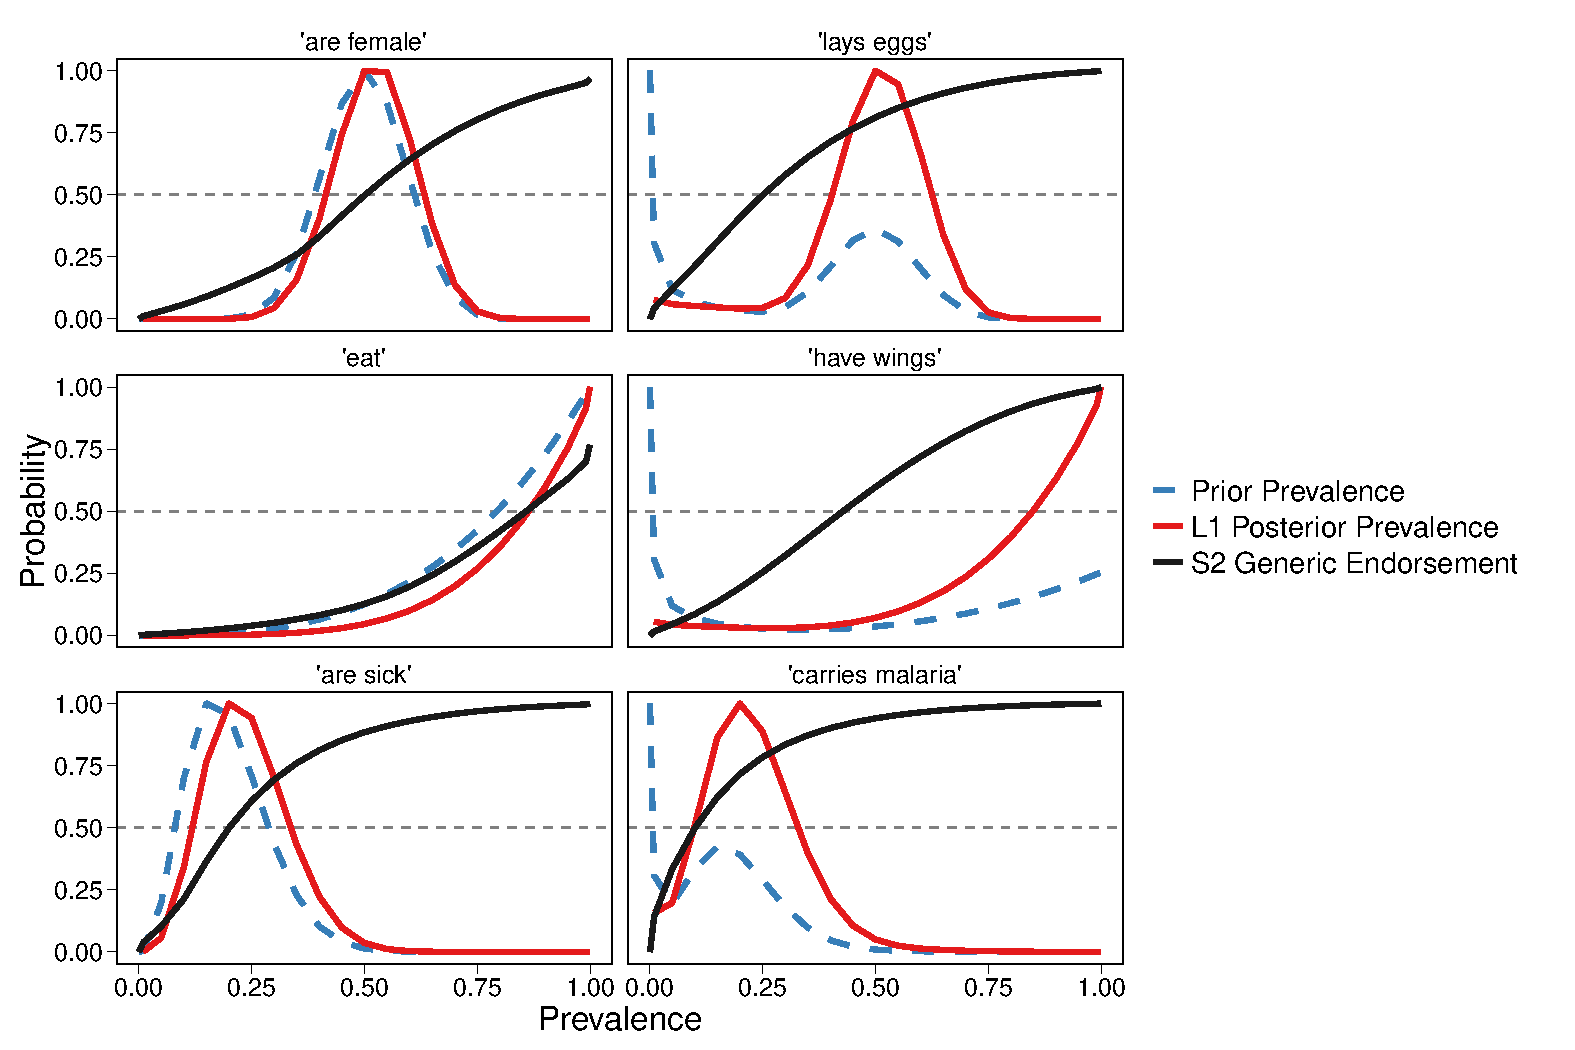
\includegraphics[width=\columnwidth]{schematics_s2.pdf}
    \caption{Schematic prior distributions for prevalence $x$ (blue dashed), the pragmatic listener $L_1$ model's posterior distribution over prevalence upon hearing a generic utterance (red), and speaker $S_2$ model's endorsement of a generic utterance for different levels of prevalence (black).
    The names given to these priors are meant to be suggestive of what kinds of properties these distributions might correspond to.
    The top row uses prevalence priors modeled as Beta(5,5), Beta(4,1), and Beta(4,16) distributions.
      The bottom row uses a prior distribution that is a mixture of the distribution above it with a second component, modeled as Beta(0.5, 4.5), reflecting categories with 0\% property prevalence.
    Horizontal dashed line at 0.5 is for convenience of comparing the point at which an utterance becomes judged as more true than false for $S_2$.
	Note that the prior distribution over prevalence will be the same as $L_1$'s posterior distribution upon hearing the ``null'' utterance.
    }
  \label{fig:schematic-unif}
\end{figure}


To take one example, consider the distribution over what might be ``are female'' (top-left facet).
\ndg{could we make the prior distribution here peakier (lower variance)? i think that matches intuitions better...}
The \emph{a priori} prevalence is centered around 0.5.
Because of pragmatics, the pressure to be \emph{truthful} will drive likely threshold values below 0.5 (lower values are more likely to be true). 
%At the same time, the maximum posterior density of the threshold is substantially greater than the lower bound. 
At the same time, the pressure to be \emph{informative} will drive the threshold values up: Higher values are more likely to be informative. 
The result is a posterior over prevalence that is somewhat greater than the prior, making higher prevalence values more likely after hearing the generic. 
But the relative information gain is very little (the posterior is not very different from the prior), and thus the $S_2$ model is reluctant to endorse the generic unless the property is especially prevalent. 
The same basic phenomenon can be observed for the other two example priors (top row): The posterior over prevalence heavily depends upon the prior, but is also not very different from the prior. %the quantitative details of this inference are heavily dependent on the shape of the prior distribution (i.e. the posteriors look dramatically different).

%Here, however, the generic interpretation ($L_1$) posterior is only slightly different from the prior. 
%This suggests there is not much information content conveyed in communicating generic statements with these kinds of priors, because the property is relatively homogeneous across all categories. 
%


%While each $P(x)$ is a single distribution on prevalence, it may be structured as the result of deeper conceptual knowledge. 
%For instance, if participants believe that some kinds have a causal mechanism that \emph{could} give rise to the property, while others do not, then we would expect $P(x)$ to be structured as a mixture distribution (cf. \citeA{Griffiths2005}).
We now imagine what would happen if there were some kinds where the property was completely absent, while being present at some rate in other kinds.
Figure \ref{fig:schematic-unif} (bottom row) shows this possibility: mixing the distribution above it with a second component at 0\% prevalence.
Consider the schematic prior over ``lay eggs''.
We see the pragmatic listener $L_1$'s posterior prevalence distribution is not very different from the interpretation that doesn't include the second component in the prior (here, ``are female''), but it is dramatically different from the prior (compare red with blue dashed line for the bottom row).
This suggests that when many categories have 0\% prevalence, lower thresholds are informative. 
Indeed, the $S_2$ model predicts that the generic becomes felicitous at lower prevalence levels (compare black line of top v. bottom row).
For ``lay eggs'', when the property is prevalent in 50\% of the kind (e.g., 50\% of birds lay eggs), endorsement of the generic (e.g., \emph{Birds lay eggs}) by the $S_2$ is roughly 0.85; for ``are female'', with the same prevalence (50\% of birds are female), endorsement for \emph{Birds are female} is only 0.50: It is judged to be neither true nor false. 
The important result is the asymmetry: the first generic can be endorsed more strongly than the second, at the same prevalence level; the exact endorsement rates depend on quantitative aspects of the priors, which must be determined empirically.
%Interestingly, the posterior distribution over prevalence $x$ (red line) is not strongly affected by this component.


%    In each case, the posterior distribution over prevalence is very different from the prior.
%    The associated endorsement probabilities for the generic are substantially higher than when that the second component is absent (compare dark line between row 1 and row 2). 
%    When the property does not exist in some number of creatures, the generic is substantially more felicitous.
%    



The model thus predicts differences in truth judgments depending on the prevalence prior. 
The first test of our theory, then, will be to see if these predictions correspond to human truth judgments of familiar generic sentences. 

%
%
%
%hears an utterance $u$, which is either a generic statement (e.g.~\emph{Robins lay eggs.}) or an uninformative \emph{null} utterance\footnote{In this case, the other thing the speaker could have done (but didn't) is said nothing, the \emph{null} utterance. 
%All results reported are similar when the alternative utterance is stipulated to be the negation---\emph{It is not the case that robins lay eggs.}---or the generic of the negation---\emph{Robins do not lay eggs.}---as opposed to the \emph{null} utterance.}.
%
 %generic utterance (\emph{Ks have F.}) from the speaker $S_{1}$ (Eq. \ref{eq:S1}). 
%
%Pragmatic interpretation of language assumes the production of an utterance was a deliberate decision on behalf of the speaker who could have said other things but didn't. 
%In order to model the interpretation of a generic utterances out of context, we assume the speaker had the options of uttering the generic utterance or staying quiet---the \emph{null utterance} alternative carries no information (i.e.~$\denote{null}(x, \theta)=T$) and produces a posterior distribution in the listener identical with the prior.\footnote{
%This alternative can be realized in at least two other ways: the speaker could have said the negation of the utterance (i.e. \emph{It is not the case that robins lay eggs.}) or the negative generic (i.e. \emph{Robins do not lay eggs.}). All results reported are similar for these two alternatives, and we use the alternative of the \emph{null} utterance for simplicity of demonstration.}
%We choose the \emph{null} utterance as the alternative in order to give the generic its communicative force; the option of staying silent makes the generic utterance into a \emph{speech-act}.



%We use $S_{2}$ (Eq.~\ref{eq:S2}) to model

%

\section*{Empirical test 1: Flexible truth conditions}

Any theory of generic language must explain their puzzling flexibility of usage with respect to prevalence.
That is, \emph{Mosquitos carry malaria} and \emph{Birds lay eggs} are reasonable things to say, but \emph{Birds are female} is not.
The pragmatic speaker model $S_2$, Eq.~\ref{eq:S2}, is a model of truth judgments. 
We test our model on thirty generic sentences 
that cover a range of conceptual distinctions discussed in the literature  \cite{Prasada2013}: characteristic (e.g. \emph{Ducks have wings.}), minority (e.g. \emph{Robins lay eggs.}), striking (e.g. \emph{Mosquitos carry malaria.}), false generalization (e.g. \emph{Robins are female.}), and false (e.g. \emph{Lions lay eggs.}).
The sentences were also chosen to elicit a range of acceptability judgments (intuitively, ``acceptable'', ``unacceptable'', and ``uncertain'') with low-, medium-, and high-prevalence properties. \ndg{last bit is redundant with methods of 1b... maybe simplify here?}

The pragmatic speaker model $S_2$ is fully-specified except for the prior distribution over prevalence $P(x)$, which plausibly varies by the type of property in question.
To compare the model to empirical truth judgments, we thus first measure the prior distribution over prevalence of these properties (Expt.~1a).
In Expt.~1b, we collect human judgements about the acceptability of the generic sentences. 

\section*{Experiment 1a: Prevalence priors}

The prior $P(x)$ (in Eqs.~\ref{eq:L1}, \ref{eq:L0}) describes the belief distribution on the prevalence of a given property (e.g. \textsc{lays eggs}) across relevant categories. 
In exploring the model, we saw that the shape of this distribution affects model predictions, and this shape may vary significantly among different properties.
We thus measured this distribution empirically for the set of properties (e.g. \textsc{lays eggs, carries malaria}; 21 in total) used in our target sentences. 
 
\subsection*{Method}

\subsubsection*{Participants}
We recruited 60 participants over Amazon's crowd-sourcing platform Mechanical Turk (MTurk).  
%We chose this number of participants based on intuition with similar experiments and model comparison; 
%since this is a quantitative experiment with no planned comparisons, power analysis in not appropriate.
Participants were restricted to those with US IP addresses and with at least a 95\% MTurk work approval rating (the same criteria apply to all experiments reported). 
3 participants where unintentionally allowed to do the experiment for a second time; we excluded their second responses (resulting in $n=57$).
2 participants self-reported a native language other than English; removing their data ($n=55$) has no effect on the results reported. 
The experiment took about 10 minutes and participants were compensated \$1.00.

\subsubsection*{Procedure and materials}
On each trial of the experiment, participants filled out a table where each row was an animal category and each column was a property. 
In order to alleviate the dependence of the distribution on our animal categories of interest, participants generated half of the animal categories before viewing the properties; the other half were randomly sampled from a set corresponding to the generic sentences used in Expt. 1b (e.g. \textsc{robins, mosquitos}).

Participants began the experiment by seeing a list of 6 animal kinds and were asked to list 5 of their own.
A column then appeared to the right of the animal names with a property in the header (e.g. ``lays eggs'').
Participants were asked to fill in each row with the percentage of members of each of the species that had the property (e.g. ``50\%'').
Eight property--columns appeared in the table, and this whole procedure was repeated 2 times.
In total, each participant generated 10 animal names and reported on the prevalence of sixteen properties for 22 animals (their own 10 and the experimentally-supplied 12). 
Properties were randomly sampled from a set of 21 properties associated with generics of theoretical interest, as described above.
% motivated by conceptual distinctions pointed out by \citeA{Prasada2013}. 
%The conceptual categories used to generate the properties (and their corresponding generics in Expt.~1b) were: majority characteristic (e.g. \emph{have spots}), minority characteristic (e.g. \emph{have manes}), striking (e.g. \emph{attack swimmers.}), and majority false generalizations (e.g. \emph{are female.}) \cite{Prasada2013}.
For a full list of the properties, and generic sentences used in Expt.~1b, see Appendix.
The experiment can be viewed at \url{http://stanford.edu/~mtessler/experiments/generics/experiments/real-kinds/prior-2.html}.

\subsection*{Data analysis and model predictions}

To process the priors data, we discretize the prevalence judgments to 12 discrete bins: $\{[0-0.01), (0.01-0.05), (0.05-0.15), (0.15-0.25),  ..., (0.75-0.85), (0.85-0.95), (0.95-1]\}$, and look at the counts within each bin, after doing add-1 Laplace smoothing, as the relative probability of that prevalence. 
Using these priors, we can explore how $P_{L_{1}}(x , \theta \mid u)$, the pragmatic listener model, interprets a generic utterance (Figure \ref{fig:commongenerics}a, insets). 
The prior beliefs over the prevalence of the property, $P(x)$, can also be interpreted as the pragmatic listener's posterior upon hearing the null utterance, because the null utterance has no information content.
We see the interpretation of the generic is quite variable across our empirically measured priors.
For instance, in the case of \textsc{carries malaria}, the prior is very left-skewed; here, the threshold $\theta$ can plausibly be quite low while still being informative, since a low threshold still rules out many possible alternative kinds (and their corresponding degree of prevalence).
Properties like \textsc{doesn't attack swimmers} are very right-skewed; here, even a relatively high threshold would not result in an informative utterance (as not many kinds would be ruled out), and so the generic is unlikely to be used by speaker $S_2$ unless the property is practically-universal within the target category. 
Some properties have priors that are unimodal with low variance (e.g. \textsc{is female}); these properties are present in every kind in almost exactly the same proportion and thus are too obvious and certain to allow for an informative generic utterance: The posterior is not very different from the prior. 
With $P(x)$ now empirically established, we can test if our speaker model predicts human truth judgments of generic statements about these properties.


\section*{Experiment 1b: Truth judgments}

%We tested the degree to which the $S_2$ model, Eq.~\ref{eq:S2}, coupled with the empirically-elicited prevalence priors from Expt.~1a predicted that a given category--property pair (e.g. \textsc{robins} and \textsc{lays eggs}) would result in a felicitous generic (e.g. \emph{Robins lay eggs.}). 


\subsection*{Method}

\subsubsection*{Participants}

We recruited 100 participants over MTurk. 
%We chose this number of participants based on intuition from similar experiments which were designed primarily to test a quantitative model.
%Participants were restricted to those with US IP addresses and with at least a 95\% MTurk work approval rating. 
4 participants were excluded for failing to pass a catch trial.
5 participants self-reported a native language other than English; removing their data has no effect on the results reported. 
The experiment took about 3 minutes and participants were compensated \$0.35.

\subsubsection*{Procedure and materials}

Participants were shown thirty generic sentences in bare plural form, one after another.
They were asked to press one of two buttons to signify whether they agreed or disagreed with the sentence (see Appendix for complete list). 
%\ndg{the order was randomized between particiapants?}
The thirty sentences were presented in a random order between participants and covered a range of conceptual categories \cite{Prasada2013}: Characteristic (e.g. \emph{Ducks have wings.}), Minority (e.g. \emph{Robins lay eggs.}), Striking (e.g. \emph{Mosquitos carry malaria.}), False generalization (e.g. \emph{Robins are female.}), and False (e.g. \emph{Lions lay eggs.}).
We also aimed to include generics that were both acceptable and unacceptable with low, medium, and high prevalence.
Approximately 10 true, 10 false, and 10 uncertain truth-value generics were selected.

As a manipulation check, participants were asked at the end of the trials which button corresponded to ``Agree''.
4 participants were excluded for failing this trial.

\subsection*{Data analysis and results}
 
 As a manipulation check, the first author assigned an \emph{a priori} truth-judgment (true/false/indeterminate) to each stimulus item.
This was a significant predictor of the empirical truth judgments: true generics were significantly more likely to be agreed with than the indeterminate generics ($\beta = 3.14; SE = 0.15; z = 21.5$), as revealed by a mixed-effect logistic regression with random by-participant effects of intercept.
Indeterminate generics were agreed with \emph{less} likely than chance ($\beta = -0.49; SE = 0.09; z = -5.3$) but significantly more than false generics ($\beta = 2.09; SE = 0.14; z = 14.5$).

 
 
 %Does subjective belief about the prevalence of the property within the target kind predict the felicity of a generic utterance?
From the prevalence prior data (Expt.~1a), we estimate participants' beliefs about the prevalence of a property \emph{for a given kind} (e.g.~the percentage of \textsc{robins} that \textsc{lay eggs}; see green intervals on Figure \ref{fig:commongenerics}a insets, and Appendix).
As a simple baseline hypothesis, we first explore whether these prevalence values themselves predict generic endorsement (e.g.~does the fraction of \textsc{robins} that \textsc{lay eggs} predict the felicity of \emph{Robins lay eggs}?).
We find a little over half of the variance in truth judgments data is explained this way ($r^2 = 0.599$; MSE=0.065; Figure \ref{fig:commongenerics}b, right). 
This is not surprising given that our stimulus set included generics that are true with high-prevalence properties (e.g. \emph{Leopards have spots.}) and  generics that are false with low prevalence properties (e.g. \emph{Leopards have wings.}). 
However, large deviations from an account based purely on target-category prevalence remain: Generics in which the target-category has intermediate prevalence (prevalence quartiles 2 and 3: $ 20\% < prevalence < 64\%$), are not at all explained by prevalence within those categories ($r_{Q2,3}^2 = 0.029$; MSE = 0.110).


%\mht{Add null model of cue validity?}

The pragmatic speaker model, $S_2$ in Eq.~\ref{eq:S2}, predicts an endorsement probability for a generic sentence, given prior beliefs about the property and a prevalence-level within the kind-of-interest. 
For the latter, we use the empirically estimated within--kind prevalence as the $x$ that the speaker $S_2$ is trying to communicate, and use the empirically measured priors from Expt.~1a as the listener's prior $P(x)$. 

\ndg{its a bit hard to follow why you're doing the things described in this paragraph. just add a bit of sign-posting? "in order to get model estimates of S2..."}
We perform our analysis bootstrapping the empirical prior data (resampling with replacement 57 participants, discretizing and binning). 
Having specified the prior $P(x)$ empirically, the pragmatic speaker has two parameters: the speaker optimality parameters $\lambda_1$ and $\lambda_2$ (in Eqs.~\ref{eq:S1}, \ref{eq:S2} ).
We infer likely values of these parameter using Bayesian data analysis \cite{LW2014}.
We put an uninformative priors over these parameters, with a range consistent with previous literature using the same model class.
%
\begin{eqnarray*}
\lambda_1 &\sim& \text{Uniform}(0,20) \\
\lambda_2 &\sim& \text{Uniform}(0,5)
\end{eqnarray*}
%
We learn about the \emph{a posteriori} credible values of our model parameter by collecting samples from MCMC chains of 10,000 iterations removing the first 5,000 iterations, using the Metropolis-Hastings algorithm. 
This was repeating 500 times for bootstrapping the prior.
The Maximum A-Posteriori (MAP) estimate and 95\% Highest Probability Density (HPD) interval for $\lambda_1$ is 0.5 [0.004, 12.7] and $\lambda_2$ is 1.7 [1.3, 2.1] (full posterior distributions can be found in Appendix B; Figure \ref{fig:tj1-params}).\footnote{
The fact that $\lambda_1$ is credibly less than 1 suggests that the generic utterance may be more costly than ``staying silent'' (our model assumes equal cost).
We maintain using only the two $\lambda$ parameters in the model for simplicity.
}

We compare the model's posterior predictive distribution of generic endorsement to the empirical truth judgments.
(The posterior predictive distribution marginalizes over the inferred parameter values to produce predictions about what the data \emph{should look like} given the pragmatics model and the observed data. 
This is akin to fitting the parameters and is the critical step in model validation: It shows what data is actually predicted by the model.) 
As we see in Figure \ref{fig:commongenerics}b, the pragmatic speaker model $S_2$, using empirically measured priors, explains nearly all of the variance in human truth judgments ($r^2=0.98$; MSE=0.003; Figure \ref{fig:commongenerics}b). 
Generics that received definitive agreement or disagreement are predicted to be judged as such by the model (corners of Figure \ref{fig:commongenerics}b), including items for which target-category prevalence is not a good indicator of the acceptability (e.g. \emph{Mosquitos carry malaria}, for prevalence quartiles 2 and 3, $r_{Q2,3}^2=0.955$; MSE=0.005; Figure \ref{fig:commongenerics}b, intermediate shades).
We also see the generics truth judgment model predicts uncertain truth judgments: for instance, \emph{Robins are female} is judged by both the model and human participants to be neither true nor false.
\emph{Sharks don't attack swimmers}, while true of most sharks, is judged to be not a good thing to say by both participants and the model.
This is strong evidence that the puzzling flexibility of generic truth-conditions can be understood with a simple semantic theory coupled with basic communicative principles (\emph{be truthful}, \emph{be informative}) operating over diverse prior beliefs about the properties, all of which are at play in understanding language. 

%\begin{figure}
%\centering
%    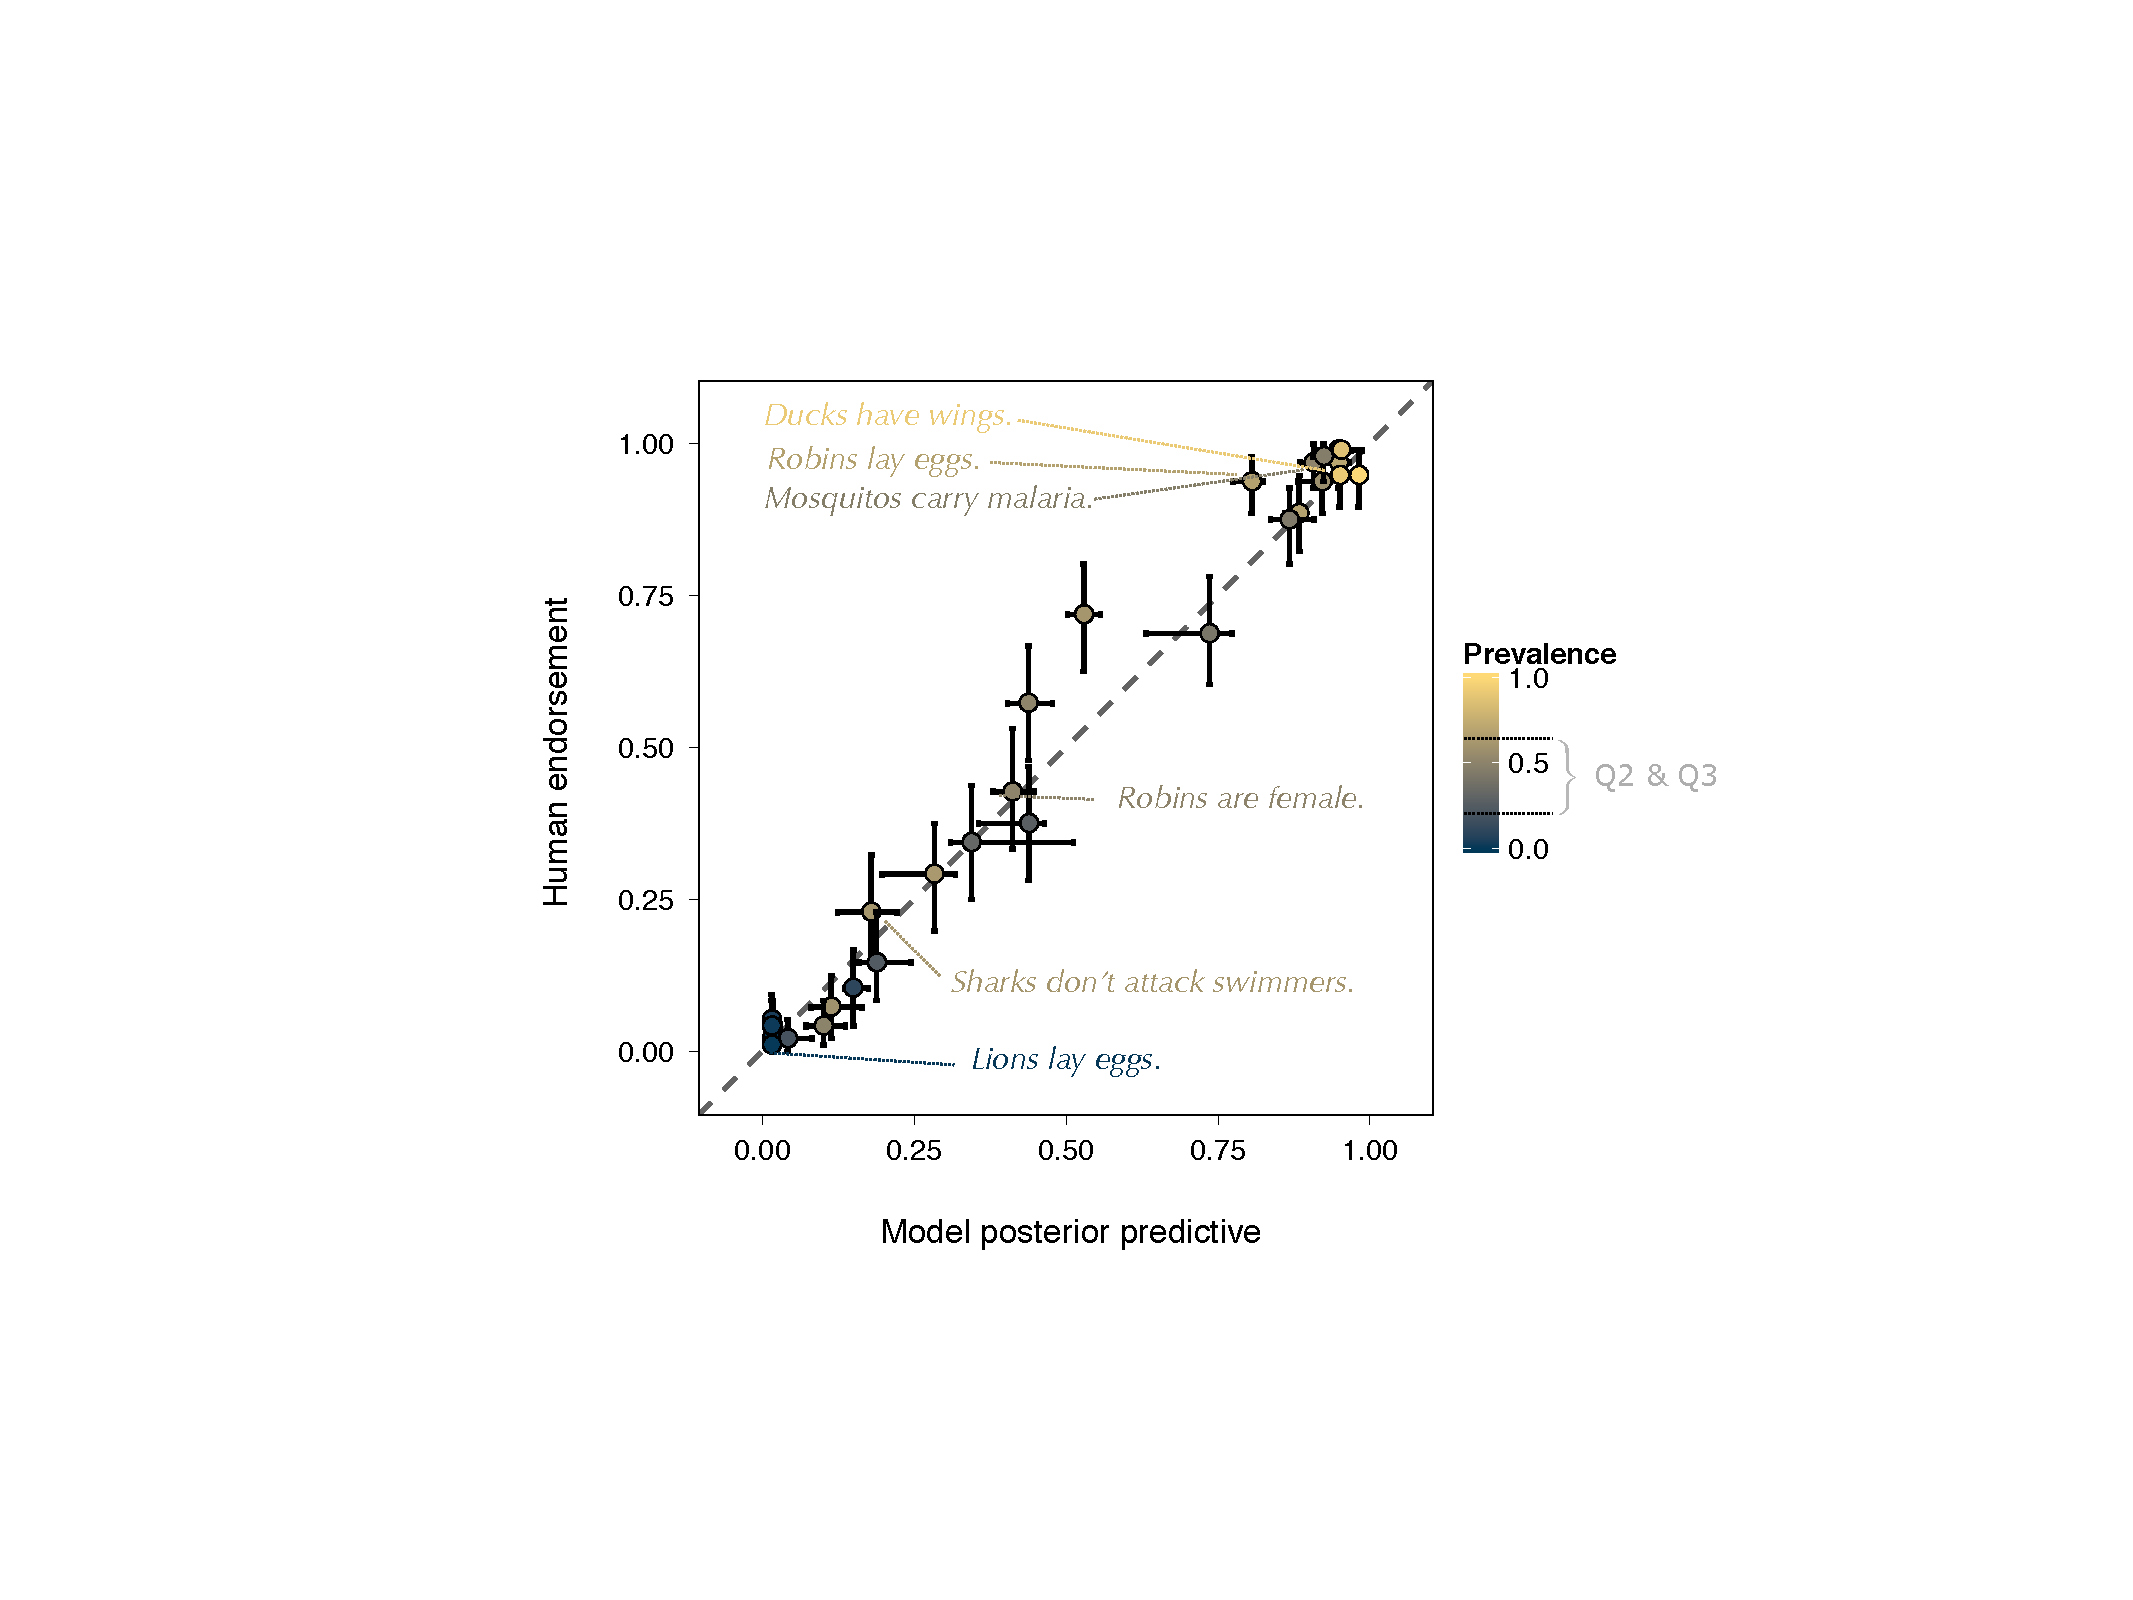
\includegraphics[width=0.7\columnwidth]{truthjudge-scatter-wLabels.pdf}
%    \caption{Human acceptability judgments and model predictions for thirty generic utterances about familiar animals and properties. 
%    Color denotes target-category prevalence of the property, with darker colors indicating lower prevalence. 
%    Intermediate prevalences (quartiles 2 \& 3) are in intermediate shades (marked on color bar).
%    Error bars correspond with 95\% bootstrapped confidence intervals for the participant data and 95\% highest probability intervals for the model predictions (same for Figures \ref{fig:impliedByItem} and \ref{fig:exp2b}).
%    }
%  \label{fig:modeldataBars}
%
%\end{figure}
%)

\begin{figure}
\centering
    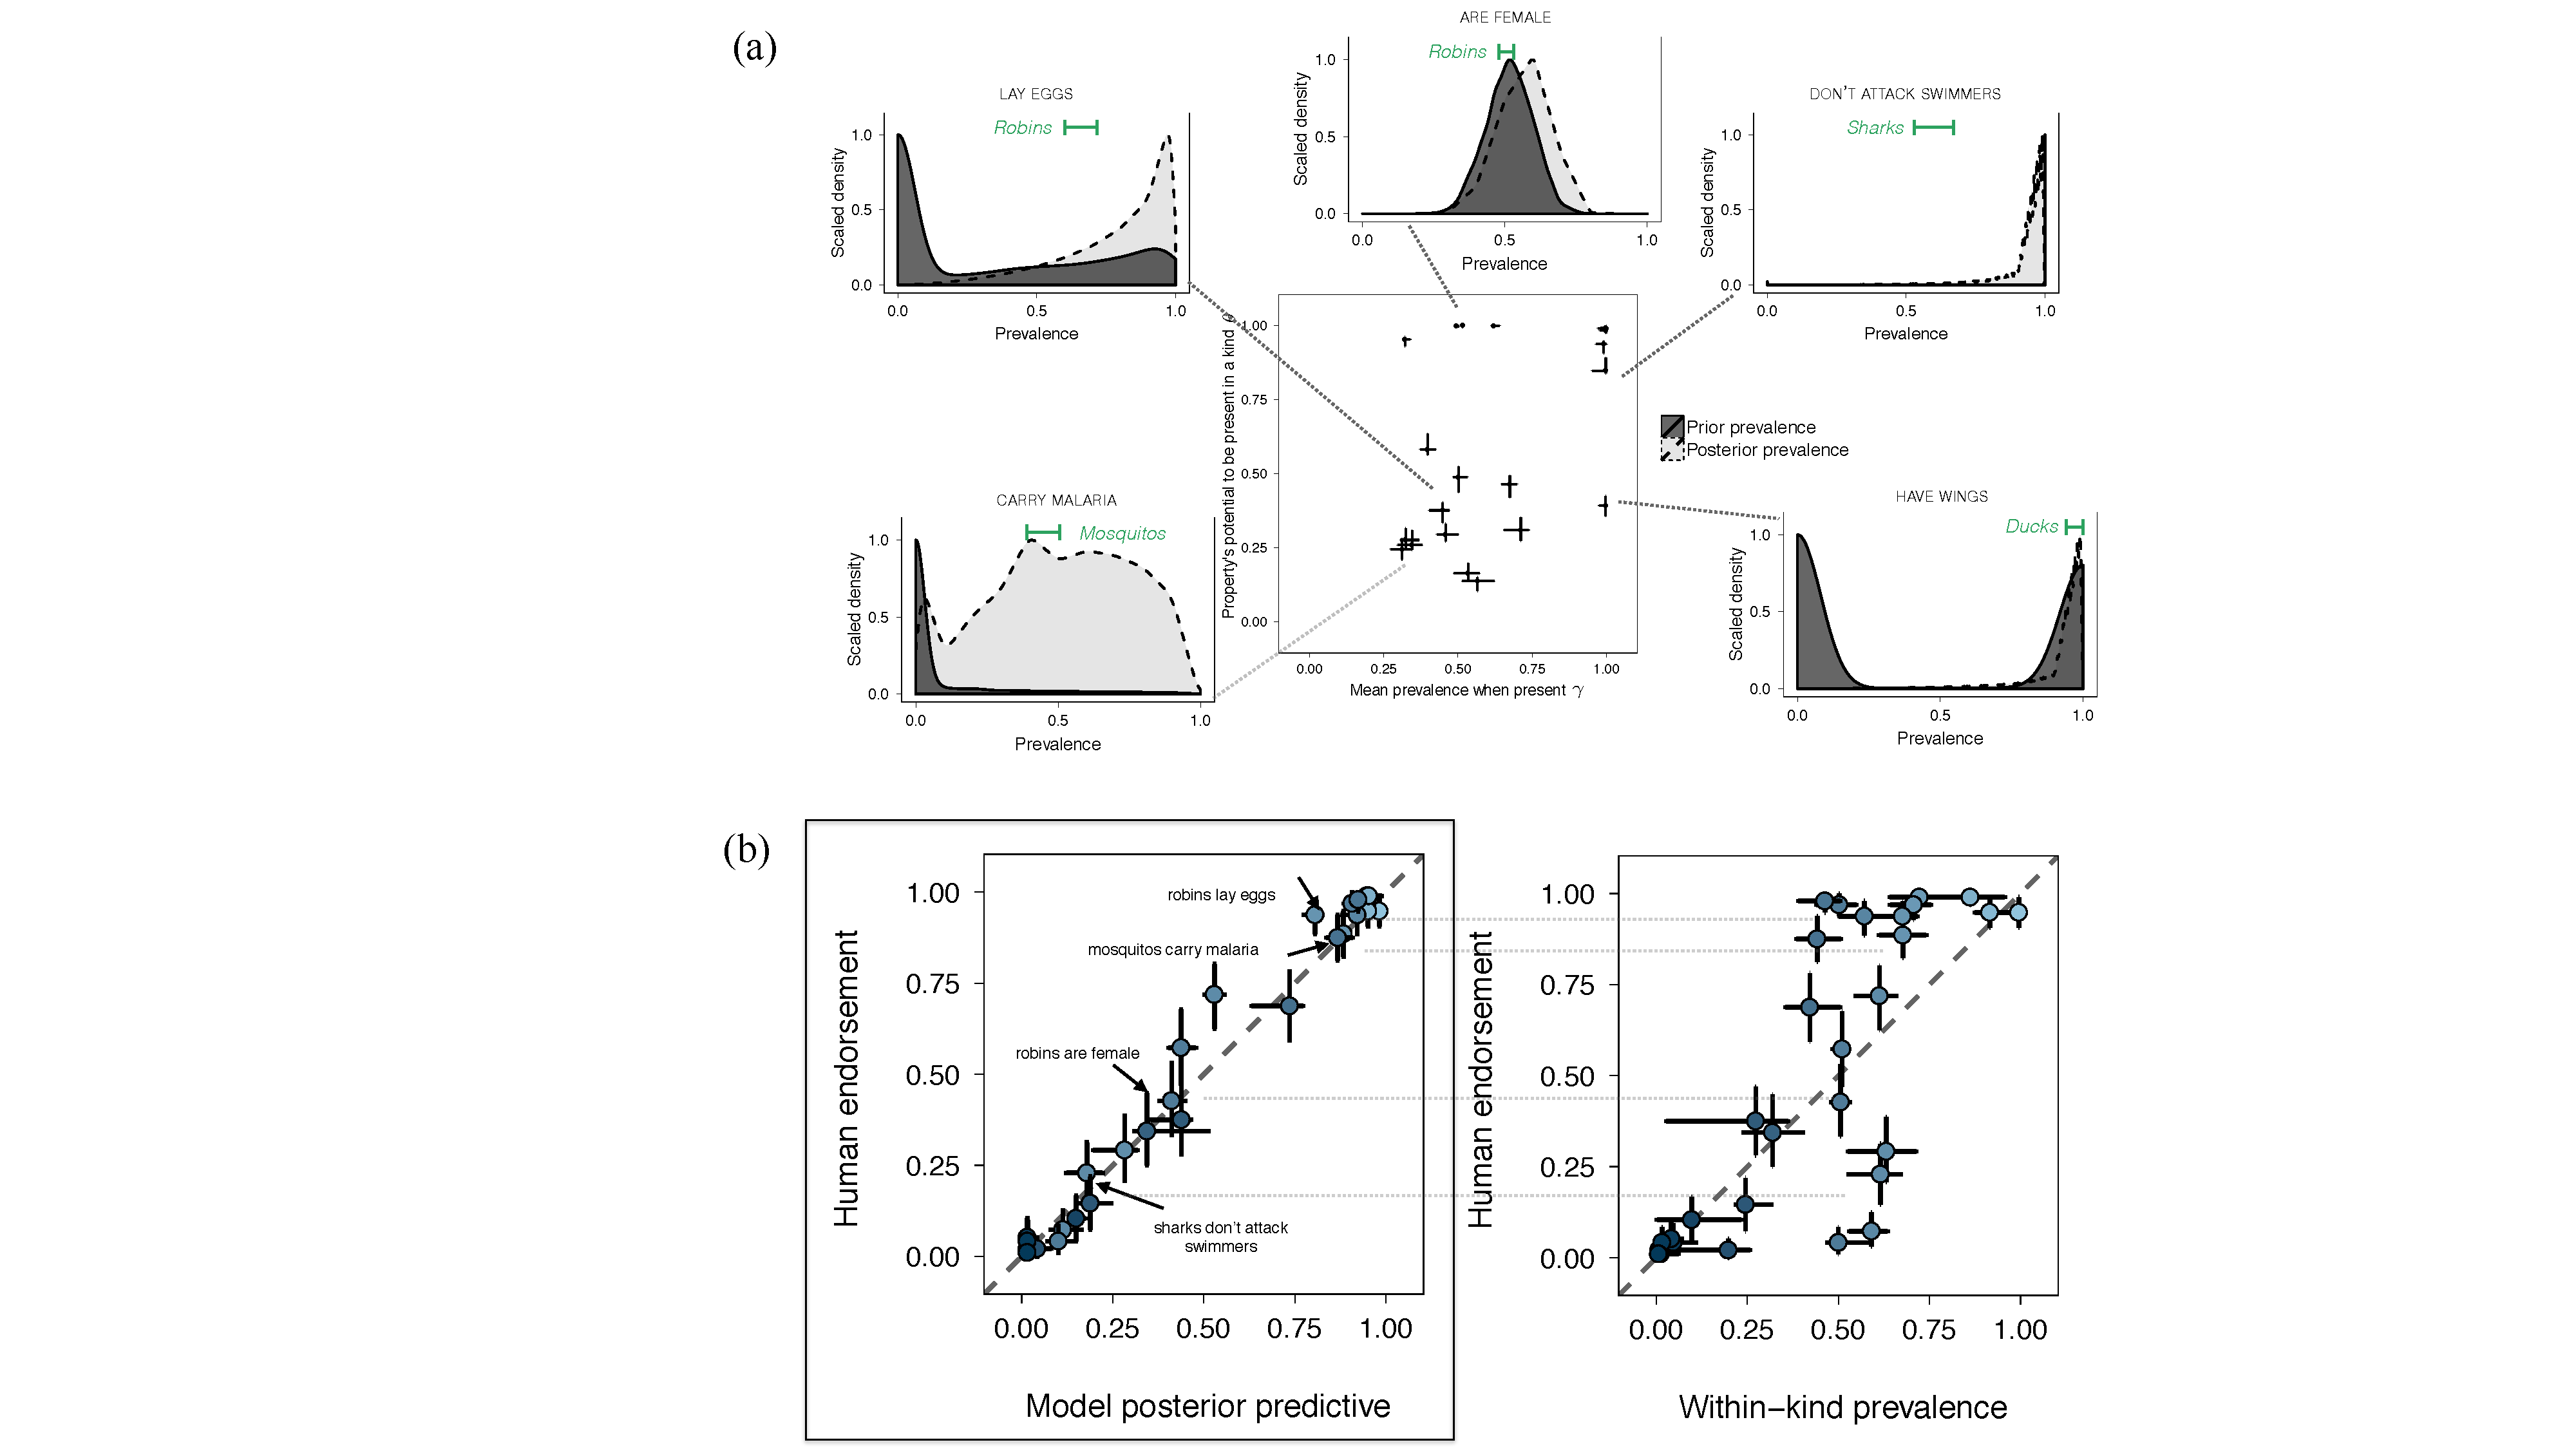
\includegraphics[width=\columnwidth]{generics-prior-prevalence-tj.pdf}
    \caption{(a) 
    Prevalence prior distributions empirically elicited for twenty-one animal properties.
    Prior distributions summarized by two parameters of a structured Bayesian model: $\phi$----a property's potential to be present in a category----and $\gamma$----the mean prevalence when it is possible for the property to be present in a category.
    Inset plots display example empirical prior distributions over prevalence and corresponding $L_1$ model predictions: the posterior after hearing a generic utterance. 
    Intervals on the top of plots show human judgments about the prevalence of the property within a target category.
    (b)
    Human acceptability judgments compared with model predictions (left) and the target-category prevalence (right) for thirty generic utterances about familiar animals and properties. 
    Color denotes target-category prevalence of the property, with darker colors indicating lower prevalence. 
     Error bars denote 95\% Bayesian credible intervals
%    Error bars correspond with 95\% bootstrapped confidence intervals for the participant data and 95\% highest probability intervals for the model predictions (same for Figures \ref{fig:impliedByItem} and \ref{fig:exp2b}).
    }
  \label{fig:commongenerics}

\end{figure}



\subsection*{Extended analysis of priors: Conceptual structure}

The pragmatics model only has a prevalence-based semantics yet it is able to explain the flexibility in truth judgments for a diverse range of generic statements.
Conceptual accounts of generic statements have looked beyond prevalence, to structured knowledge representations as the critical factor in generic meaning \cite{Leslie2007, Prasada2013}. 
We can interrogate our formal model to see what is driving its predictions, and, in particular, we ask whether structured representations might effect our model after all.

For a given property,  the prior distribution on prevalence $P(x)$ is a single distribution.
However, the distribution may be structured as the result of deeper conceptual knowledge. 
For instance, if participants believe that some kinds have a causal mechanism that \emph{could} give rise to the property, while kinds others do not, then we would expect $P(x)$ to be structured as a mixture distribution (cf. \citeA{Griffiths2005}).
We know that prior knowledge plays a fundamental role in leading the pragmatics model endorse or reject generics. 
We now explore the hypothesis that this is at least partly because these priors are structured into two components: kinds that \emph{can} have the property and other kinds that \emph{cannot}.
%The minimal evidence for a structured representation within the elicited priors would be a mixture distribution, where the underlying prevalence distribution is actually mixture of two distributions. 
We explore this possibility by formulating a mixture model for the prevalence priors, and exploring how well it fits the data from elicited in Expt.~1a.
%
%We do this by formulating such 
%further analyzing the prevalence prior data from Expt.~1a.

\subsubsection*{Data analysis}

If a kind can have the property, we assume the prevalence follows a Beta distribution with mean $\gamma$ and concentration $\xi$. 
If a kind cannot, we assume the prevalence is a Delta distribution, with all probability mass at 0\%.\footnote{There are other ways to formulate the second component (``the kind doesn't have a causal mechanism that would give rise to  the property'') of the prior. 
It could reflect accidental causes of the property, in which case, the prevalence could be a distribution that allows for non-zero prevalence. 
While an interesting possibility, its full consideration is beyond the scope of this article.
}
The relative contribution of these two components is governed by mixture parameter $\phi$, inferred from the data.\footnote{This is similar in spirit to Hurdle Models of epidemiological data, where the observed count of zeros is often substantially greater than one would expect from standard models, such as the Poisson (e.g. adverse events to vaccines)\cite{hurdleModels}}
We think of $\phi$ the \emph{potential of a property to be present in a kind} and $\gamma$ is the \emph{mean prevalence of the property among the kinds with the potential to have it}.\footnote{We note that $\phi$ is not what other authors have described as \emph{cue validity} \ndg{cite?}, or $P(K \mid F)$. 
$\phi$ is a mixture component in the distribution over $P(F\mid K$).
}
If this model is correct, the prevalences given by participants would then be distributed as: $P(d) = \phi \cdot \text{Beta}(d \mid \gamma,\xi)+ (1 - \phi) \cdot \delta_{d=0} $. 



%\mht{Add a sentence or a footnote about how $\theta$ is not the same as cue validity.} 
%\ndg{i think we need only the second equation, but write as probability. and x should be d}
%\mht{is this a "written as a probability"?}
%\begin{align*}
%%	d_{observed} & \sim \begin{cases}
%%				 \text{Beta}(\gamma, \xi) & \mbox{if } \text{Bernoulli}(\theta) = \textsc{t}  \\
%%				 \delta_{x=0} & \mbox{if }\text{Bernoulli}(\theta) = \textsc{f} \\
%%				\end{cases} \\
%%	 d_{observed} &  \sim \theta \cdot \beta(\gamma,\xi)+ (1 - \theta) \cdot \delta_{d=0} 
%	 P(d) = \theta \cdot \text{Beta}(d \mid \gamma,\xi)+ (1 - \theta) \cdot \delta_{d=0} 
%\end{align*}
We performed Bayesian inference over this model, given the observed prevalence data, to examine how well the model's posterior predictive distribution reconstructs the prevalence prior data.
We put uninformative priors over all the parameters, $\phi \sim \text{Uniform}(0,1)$, 
$\gamma \sim \text{Uniform}(0,1)$, $\xi \sim \text{Uniform}(0, 50)$, 
and performed Bayesian inference separately for each property using the Metropolis-Hastings algorithm 
%to estimate the posterior distribution over the latent parameters $\phi, \gamma$, and $\xi$ 
collecting 50,000 samples removing the first 25,000 iterations for burn-in.

\subsubsection*{Results}


Estimates of the mixture parameter $\phi$ and the mean of the ``has the potential'' component $\gamma$ for each property are shown in Figure \ref{fig:commongenerics}a.
We see significant diversity among our properties in both parameters, corresponding to priors over prevalence with dramatically different shapes (insets). 

Again, we look to the posterior predictive distribution to validate the structured prior model.
Using the model with its inferred parameters, we generate prevalence judgments for different properties and compare that to the empirical counts. 
%\mht{Instead: make a quantile--quantile (ie cdf vs. cdf) plot?}
We discretize the prevalence values of both the model and the data to 12 discrete bins: $\{[0-0.01), (0.01-0.05), (0.05-0.15), (0.15-0.25),  ..., (0.75-0.85), (0.85-0.95), (0.95-1]\}$.
This statistical model reproduces the prior elicitation data very well ($r^2 = 0.94$), strongly supporting the possibility of a structured prior. 
\ndg{give fit of single component version for comparison?}

The other test of this hypothesis is to re-examine the truth judgments from Expt.~1b using the pragmatics model with the inferred structured priors (as opposed to bootstrapping the raw empirical counts). 
We find the same correspondence to the empirical truth judgments data ($r^2 = 0.98$).
This provides further evidence that the prior distribution over prevalence $P(x)$ is structured.
The implication of this finding is that conceptual structure may indeed find its way into generic judgements, but via the prevalence prior, rather than directly in the semantics of the generic. We return to this idea \ndg{below}.

%The only substantial disagreement between the prior model and the data occur for  the properties \textsc{is male, is female} in the bin $(0.45-0.55)$. 
%The normalized empirical counts put about 75\% probability in this bin; the model predicts roughly 50\% probability of this bin. 
%This discrepancy can be attributed to a number of 100\% or 0\% responses present in the data (e.g. some participants self-generated the category \textsc{cow}, and rated that 100\% of cows are female). 
%Since the model assumes a smooth Beta distribution, these responses work to flatten out the distribution.

\begin{figure}
\centering
    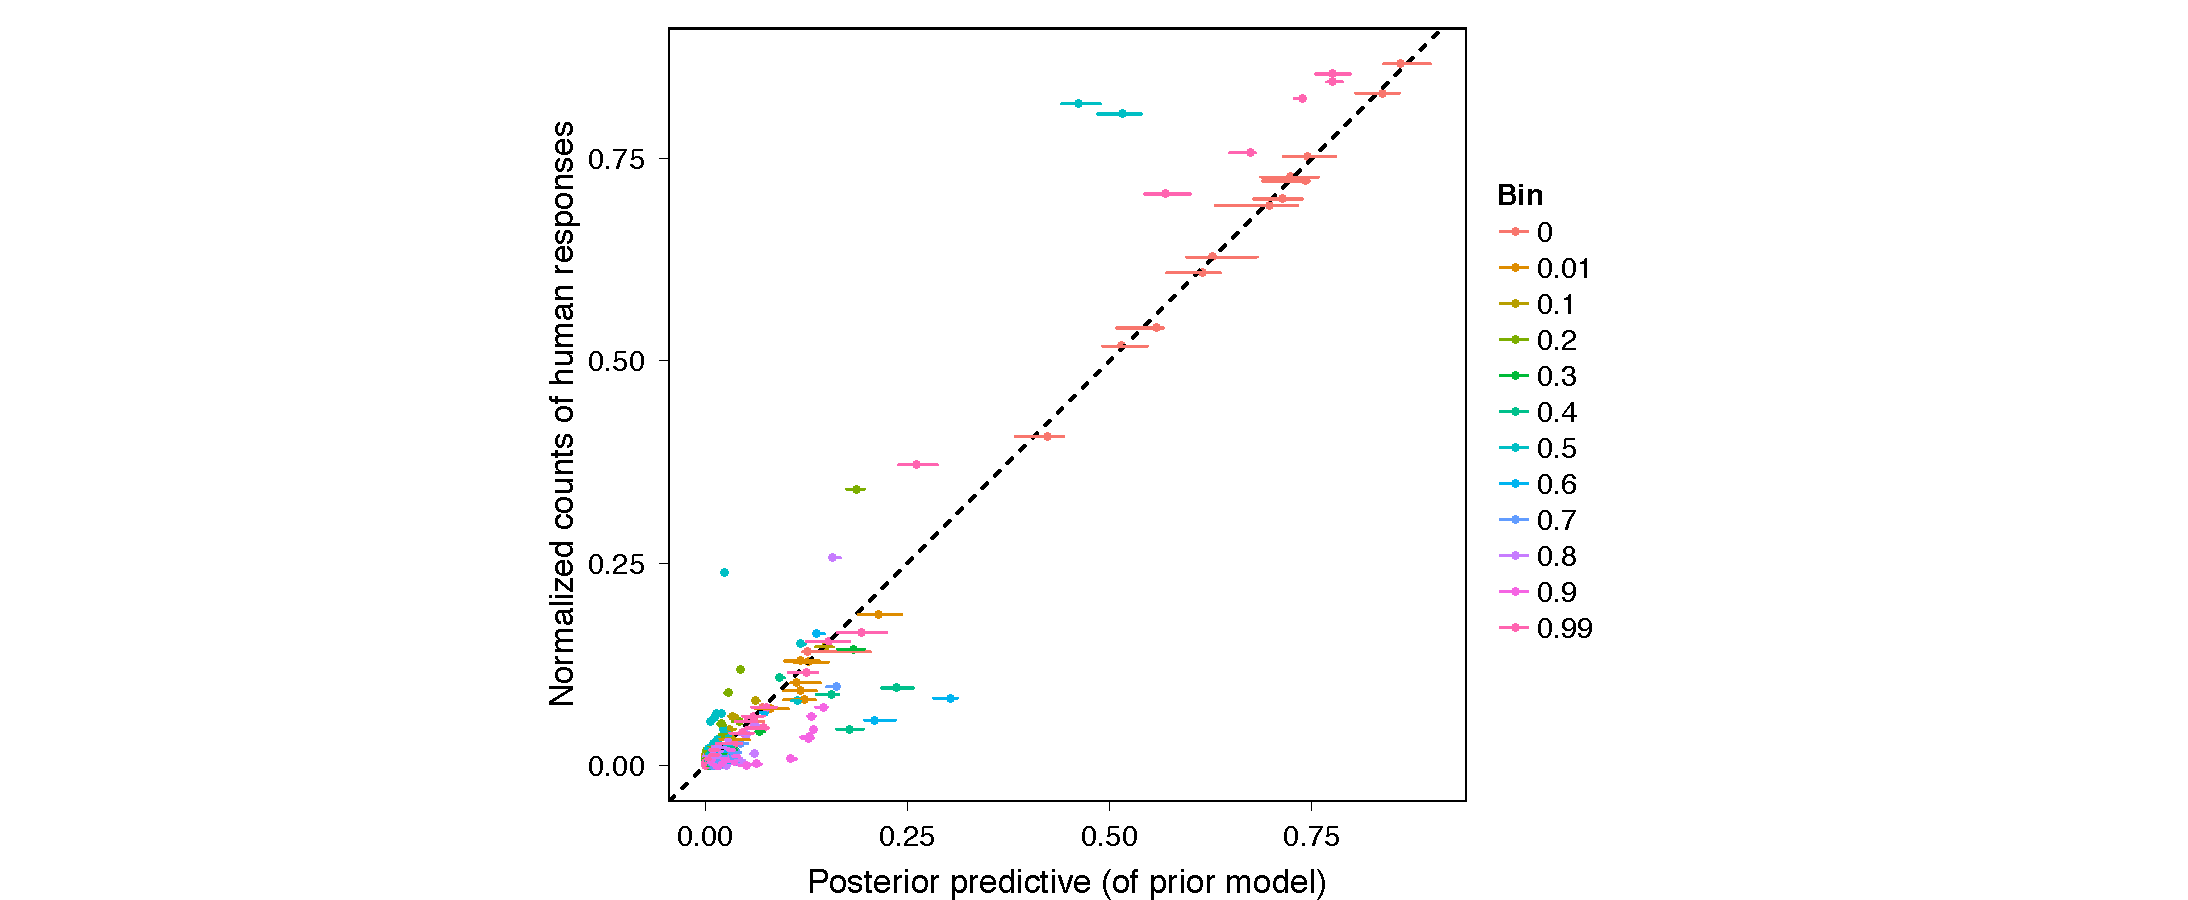
\includegraphics[width=0.6\columnwidth]{postPred-priorModel.pdf}
    \caption{Posterior predictive distribution of the structured, statistical model thought to give rise to the human data in the prior elicitation task. The close alignment between model and data suggests the assumption of a structured prior is warranted.}
  \label{fig:pp-priorModel}
\end{figure}

%\subsection*{Results}

%Using this structure, we can explore our twenty-one properties:
%Figure \ref{fig:priors1a} shows the estimated mixture-parameter $\theta$ (the potential of the property to be present in a kind) and the mean prevalence when the property is present, $\gamma$. 
%We see significant diversity among these properties in both dimensions, resulting in priors over prevalence with dramatically different shapes (insets). 
%This diversity matters because the model predictions for generic interpretation and felicity depend on the shape of the prior distribution (insets show example $L_1$ interpretation posteriors).
%Lowering $\theta$ effectively makes the property more distinctive by increasing the relative probability mass at 0\%; this relaxes the truth conditions by making a lower threshold more informative.\mht{Make a comment how $\theta$ is not the same as cue-validity?}.
%Increasing $\gamma$ means the property is expected to be present in more members of the category; this tends to make truth conditions stricter, by reducing the range of prevalence values higher than the prior expectation. 

%
%\begin{figure*}
%%\floatbox[{\capbeside\thisfloatsetup{capbesideposition={right,top},capbesidewidth=4cm}}]{figure}[\FBwidth]
%%{\caption{A test figure with its caption side by side}\label{fig:test}}
%\centering
%    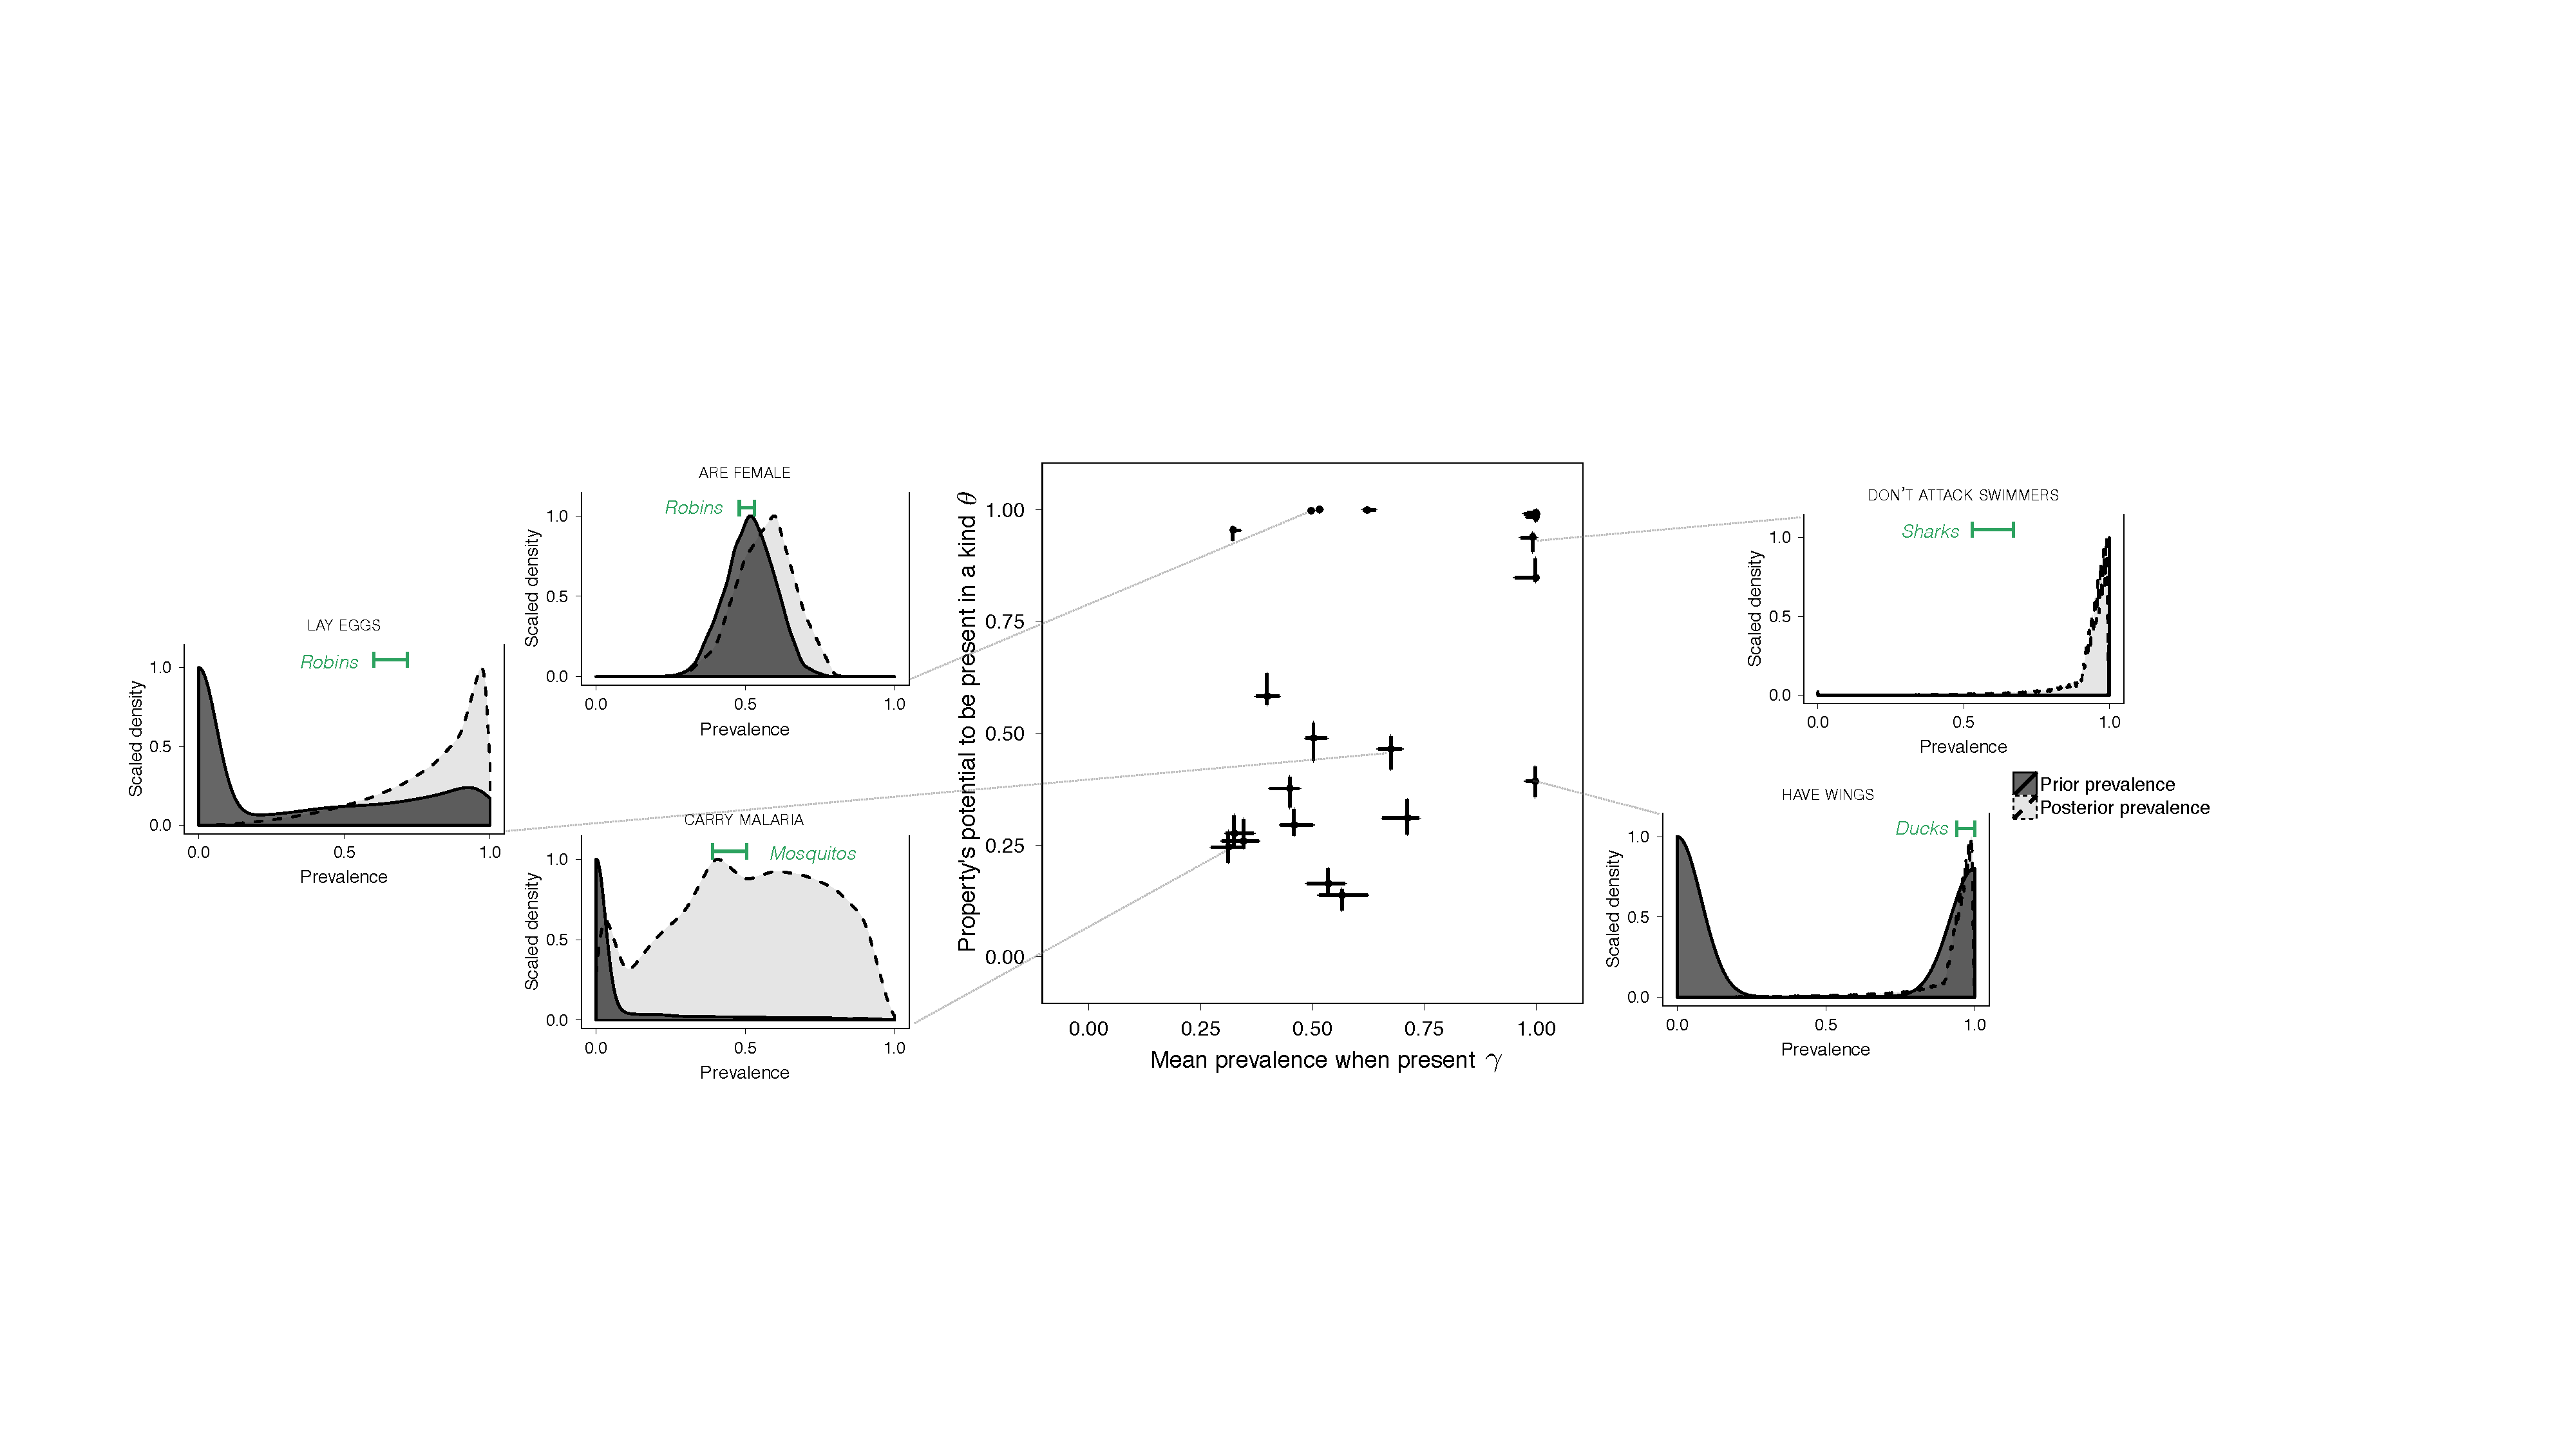
\includegraphics[width=\columnwidth]{prevalence-scatter-wDists_wide.pdf}
%    \caption{Prevalence prior distributions empirically elicited for twenty-one animal properties.
%    Prior distributions are summarized by $\theta$----a property's potential to be present in a category----and $\gamma$----the mean prevalence when it is possible for the property to be present in a category.
%    Inset plots display example empirical prior distributions over prevalence together with corresponding $L_1$ model predictions: the posterior after hearing a generic utterance. 
%    Intervals on the top of plots show human beliefs about the prevalence of the property within a target category.
%%    Posterior distributions show what happens to a listener's belief about the prevalence after hearing the associated generic. 
%    Felicitous generic utterances result when the target prevalence is more likely under the posterior than under the prior.
% %   \ndg{should mark the observed within-category prevalence for target kinds in pop-outs? or maybe one of the axes of main plot should be that?}
%     Error bars denote 95\% Bayesian credible intervals (same for Figure \ref{fig:prior2}).
%    }
%  \label{fig:priors1a}
%\end{figure*}





\section*{Empirical test 2: Interpreting novel generics}

One of the most important roles for generic language is to provide learners information about new or poorly understood categories. 
This role depends on how unfamiliar generic sentences are interpreted \cite<e.g.>{Gelman2002, Cimpian2010}.
The pragmatic theory we present includes such a theory of generic comprehension: the listener model (Eq.~\ref{eq:L1}) describes interpretation of a generic utterance---\emph{Feps \textsc{have property}}---without previously knowing the prevalence of the property within this kind.
In our theory, the meaning is uncertain, but the pressure to be informative operates over \emph{a priori} beliefs about properties to produce an interpretation. 
Classic work in generalization suggests beliefs about the prevalence of properties differ by type of property, including relatively fine distinctions among properties that are all biological in nature \cite{Nisbett1983}. 
We leverage these diverse expectations, using properties that explore a wide range of \emph{a priori} beliefs about prevalence. 

Measuring \emph{a priori} beliefs is tricky when the kinds are unknown.
We cannot, as before, have participants fill out a table with rows corresponding to different animal kinds and columns corresponding to different properties:  Nothing would distinguish the rows.
Instead, we leverage the latent structure uncovered in our extended model analysis of Expt.~1 and decompose prevalence priors into 2 components: the property's potential to be present in a kind and the mean prevalence when present.

We use this novel method for measuring \emph{a priori} beliefs about the prevalence of these properties for unfamiliar kinds (Expt.~2a).
We then test the predictions of the pragmatic listener model $L_1$ using these empirically derived priors against human \emph{interpretations} of novel generic sentences (Expt.~2b).
Finally, we explain a previously reported empirical asymmetry between truth conditions and interpretations by comparing the speaker $S_2$ and listener $L_1$ models in the same experimental context (Expt.~2c).


%These items make up four categories of properties: body parts of a particular color (e.g. \textsc{has green feathers}), described vaguely (e.g. \textsc{has small wings}), in accidental or disease states (e.g. \textsc{has wet fur}, \textsc{has swollen ears}), and without modification (e.g. \textsc{has claws}).


\section*{Experiment 2a: Prevalence priors for unfamiliar kinds}

%To measure the prior over prevalence using \emph{familiar} categories (Expt. 1a), participants filled out a table with rows corresponding to different animal kinds and columns corresponding to different properties.
%We cannot do the same for unfamiliar kinds:
%% (What percentage of feps have yellow fur?)
%%But without reference to a familiar kind, how can one know what prevalence to expect? 
%We instead 
%This suggests a two-stage elicitation procedure.
%
% we discovered a latent structure to the prevalence priors task.
%A simple, structured Bayesian model easily accommodated the data using two components: the property's potential to be present in a kind and the expected prevalence when present.
%We leveraged this structure to measure prevalence priors with unfamiliar categories. 

%, structuring our task into questions about the property's potential to be present in a kind and the expected prevalence when present; we then used a Bayesian statistical model to reconstruct the underlying prior distribution. 
%
%
%
%Pilot testing suggested this was a pragmatically strange setup when using novel kinds: answering ``What percentage of lorches have green feathers?'', when participants knew nothing about lorches, was difficult.

\subsection*{Method}

\subsubsection*{Participants}

We recruited 40 participants over MTurk.  
%We again chose this number of participants based on intuition from similar experiments which were designed primarily to test a quantitative model.
%Participants were restricted to those with US IP addresses and with at least a 95\% MTurk work approval rating. 
All participants were native English speakers. 
The experiment took about 5-7 minutes and participants were compensated \$0.75.

\subsubsection*{Procedure and materials}

%Classic work in generalization suggests beliefs about the prevalence of properties differ by type of property, including relatively fine distinctions between properties that are all biological in nature \cite{Nisbett1983}. 
We constructed forty different properties to explore a wide range of \emph{a priori} beliefs about prevalence. 
These items make up four categories of properties: body parts of a particular color (e.g. \textsc{has green feathers}), described vaguely (e.g. \textsc{has small wings}), in accidental or disease states (e.g. \textsc{has wet fur}, \textsc{has swollen ears}), and without modification (e.g. \textsc{has claws}).
%\footnote{The distinction between common and rare accidental properties was determined empirically by analyzing the data by item, and performing a median split based on the \emph{a priori} mean prevalence when present, $\gamma$, of the property.}.
%We are interested in testing in the predictive power of 
Because pilot testing revealed more variability for items in the accidental category relative to the other types of properties, we used twice as many exemplars of accidental properties, yielding a more thorough test of the quantitative predictive power of the $L_1$ interpretation model. 
We used 8 exemplars of each of the three non-accidental properties (``parts'', ``colored parts'', ``vague parts''), and 16 exemplars of accidental properties, building on a stimulus set from \citeA{Cimpian2010}.
All materials are shown in the Appendix.

Participants were introduced to a ``data-collection robot'' that was tasked with learning about properties of animals. 
Participants were told the robot randomly sampled an animal to ask the participant about (e.g. The robot says: ``We recently discovered animals called feps.''). 
We then used a two-stage elicitation procedure, aimed to measure the two components of the structured prior model: (1) the potential of the property to be present in a kind and (2) the expected prevalence when present.
To get at (1), the robot asked how likely it was that ``there was \emph{a} fep with \textsc{property}'' (potential to be present), to which participants reported on a scale from ``unlikely'' to ``likely''.
For example, it is very likely that there is a fep that is female, less likely that there is a fep that has wings, and even less likely that there is a fep that has purple wings. 
To get at (2), the robot then asked, ``Suppose there is a fep that has wings. What percentage of feps do you think have wings?'' (expected prevalence when present). 
Participants completed a practice trial to make sure they understood the meanings of these two questions.

%responded using slider bars for each question.
%
%$P(x)$ was measured empirically ($n=40$, {\it Experiment 2a}), and the most likely priors were inferred using the same structured, statistical approach used for the familiar generics experiment.

\subsection*{Data analysis and results}

We used the same structured, statistical model for the prior data from Expt.~1.
The only difference from Expt.~1a. is that our experimental data comes from inquiring about the parameters of the priors directly, as opposed to asking about particular samples from the prior (i.e. particular kinds) as was done in Expt.~1a. 
%For Expt.~2a, participants are asked questions directly targeting $\theta$ and $\gamma$ in the above model (see {\it Expt. 2a}).
We assume these two measurements follow Beta distributions ($d_{potential} \sim \text{Beta}(\gamma_{1}, \xi_{1})$; $
d_{expected} \sim \text{Beta}(\gamma_{2}, \xi_{2})$), and construct single prevalence distributions, $P(x)$, by sampling from the posterior predictive distribution of prevalence as we did before: $P(x) = \int [ \phi\cdot \text{Beta} (x \mid \gamma_{2}, \xi_{2}) + (1 -  \phi) \cdot \delta_{x=0} ] \cdot \text{Beta}(\phi \mid \gamma_{1}, \xi_{1}) d\phi$.
We used the same uninformative priors over parameters $\phi, \gamma_{i}, \xi_{i}$ as in Expt.~1a.
%
%\begin{minipage}{0.5 \textwidth} \small
%\begin{align*}
%%\end{align*}
%%%\end{minipage}
%%%
%%To %\begin{minipage}{0.5 \textwidth} \small
%%%        \begin{align*}
%%\theta & \sim \text{Beta}(\gamma_{potential}, \xi_{potential}) \\ 
%P(x) = [ \theta\cdot \text{Beta} (x \mid \gamma_{2}, \xi_{2}) + (1 -  \theta) \cdot \delta_{x=0} ] \cdot \text{Beta}(\theta \mid \gamma_{1}, \xi_{1})
%%
%%\begin{cases} 
%%		\text{Beta}(\gamma_{expected}, \xi_{expected}) &\mbox{if } \text{Bernoulli}(\theta) = \textsc{t} \\
%%				\delta_{x=0} &\mbox{if } \text{Bernoulli}(\theta) = \textsc{f} \\
%%		\end{cases} \\
%\end{align*}
%%\ndg{this eqn is kind of ugly. simplify in coordination with the earlier one?}
%
%%	 P(d_{observed} ) = \theta \cdot \beta(\gamma,\xi)+ (1 - \theta) \cdot \delta_{d=0} 


Figure \ref{fig:prior2}a shows a summary of the elicited priors, in terms of the diversity of $d_{potential}$ and $d_{expected}$.
Biological properties are expected to be \emph{a priori} more prevalent within a kind when present than accidental properties, with additional fine-grained differences within biological and accidental properties.
Like the priors elicited using familiar categories, these priors elicited using unfamiliar categories have diverse shapes (see insets). 
Biological properties (``biological'', ``vague'', and ``color'' body parts) have prevalence distributions that are bimodal with peaks at 0\% and near-100\% prevalence. 
Interpretations of generics about these properties ($L_1$ model, Eq.~\ref{eq:L1}) update these distribution to concave posteriors peaked at 100\% (Figure \ref{fig:prior2}; red, blue and green insets); the model predicts these novel generics will be interpreted as implying the property is widespread in the category \cite{Gelman2002}.
By contrast, accidental properties (both ``rare'' and ``common'') follow unimodal prior distributions and update to convex posterior distributions, predicting weaker and more variable interpretations of novel generics for these properties \cite{Cimpian2010c}. 
%These convex posteriors show that generics about accidental or temporary properties come with highly uncertain interpretations, plausibly as a consequence of theory-driven considerations \cite{Cimpian2010c}. 


\begin{figure*}
\centering
    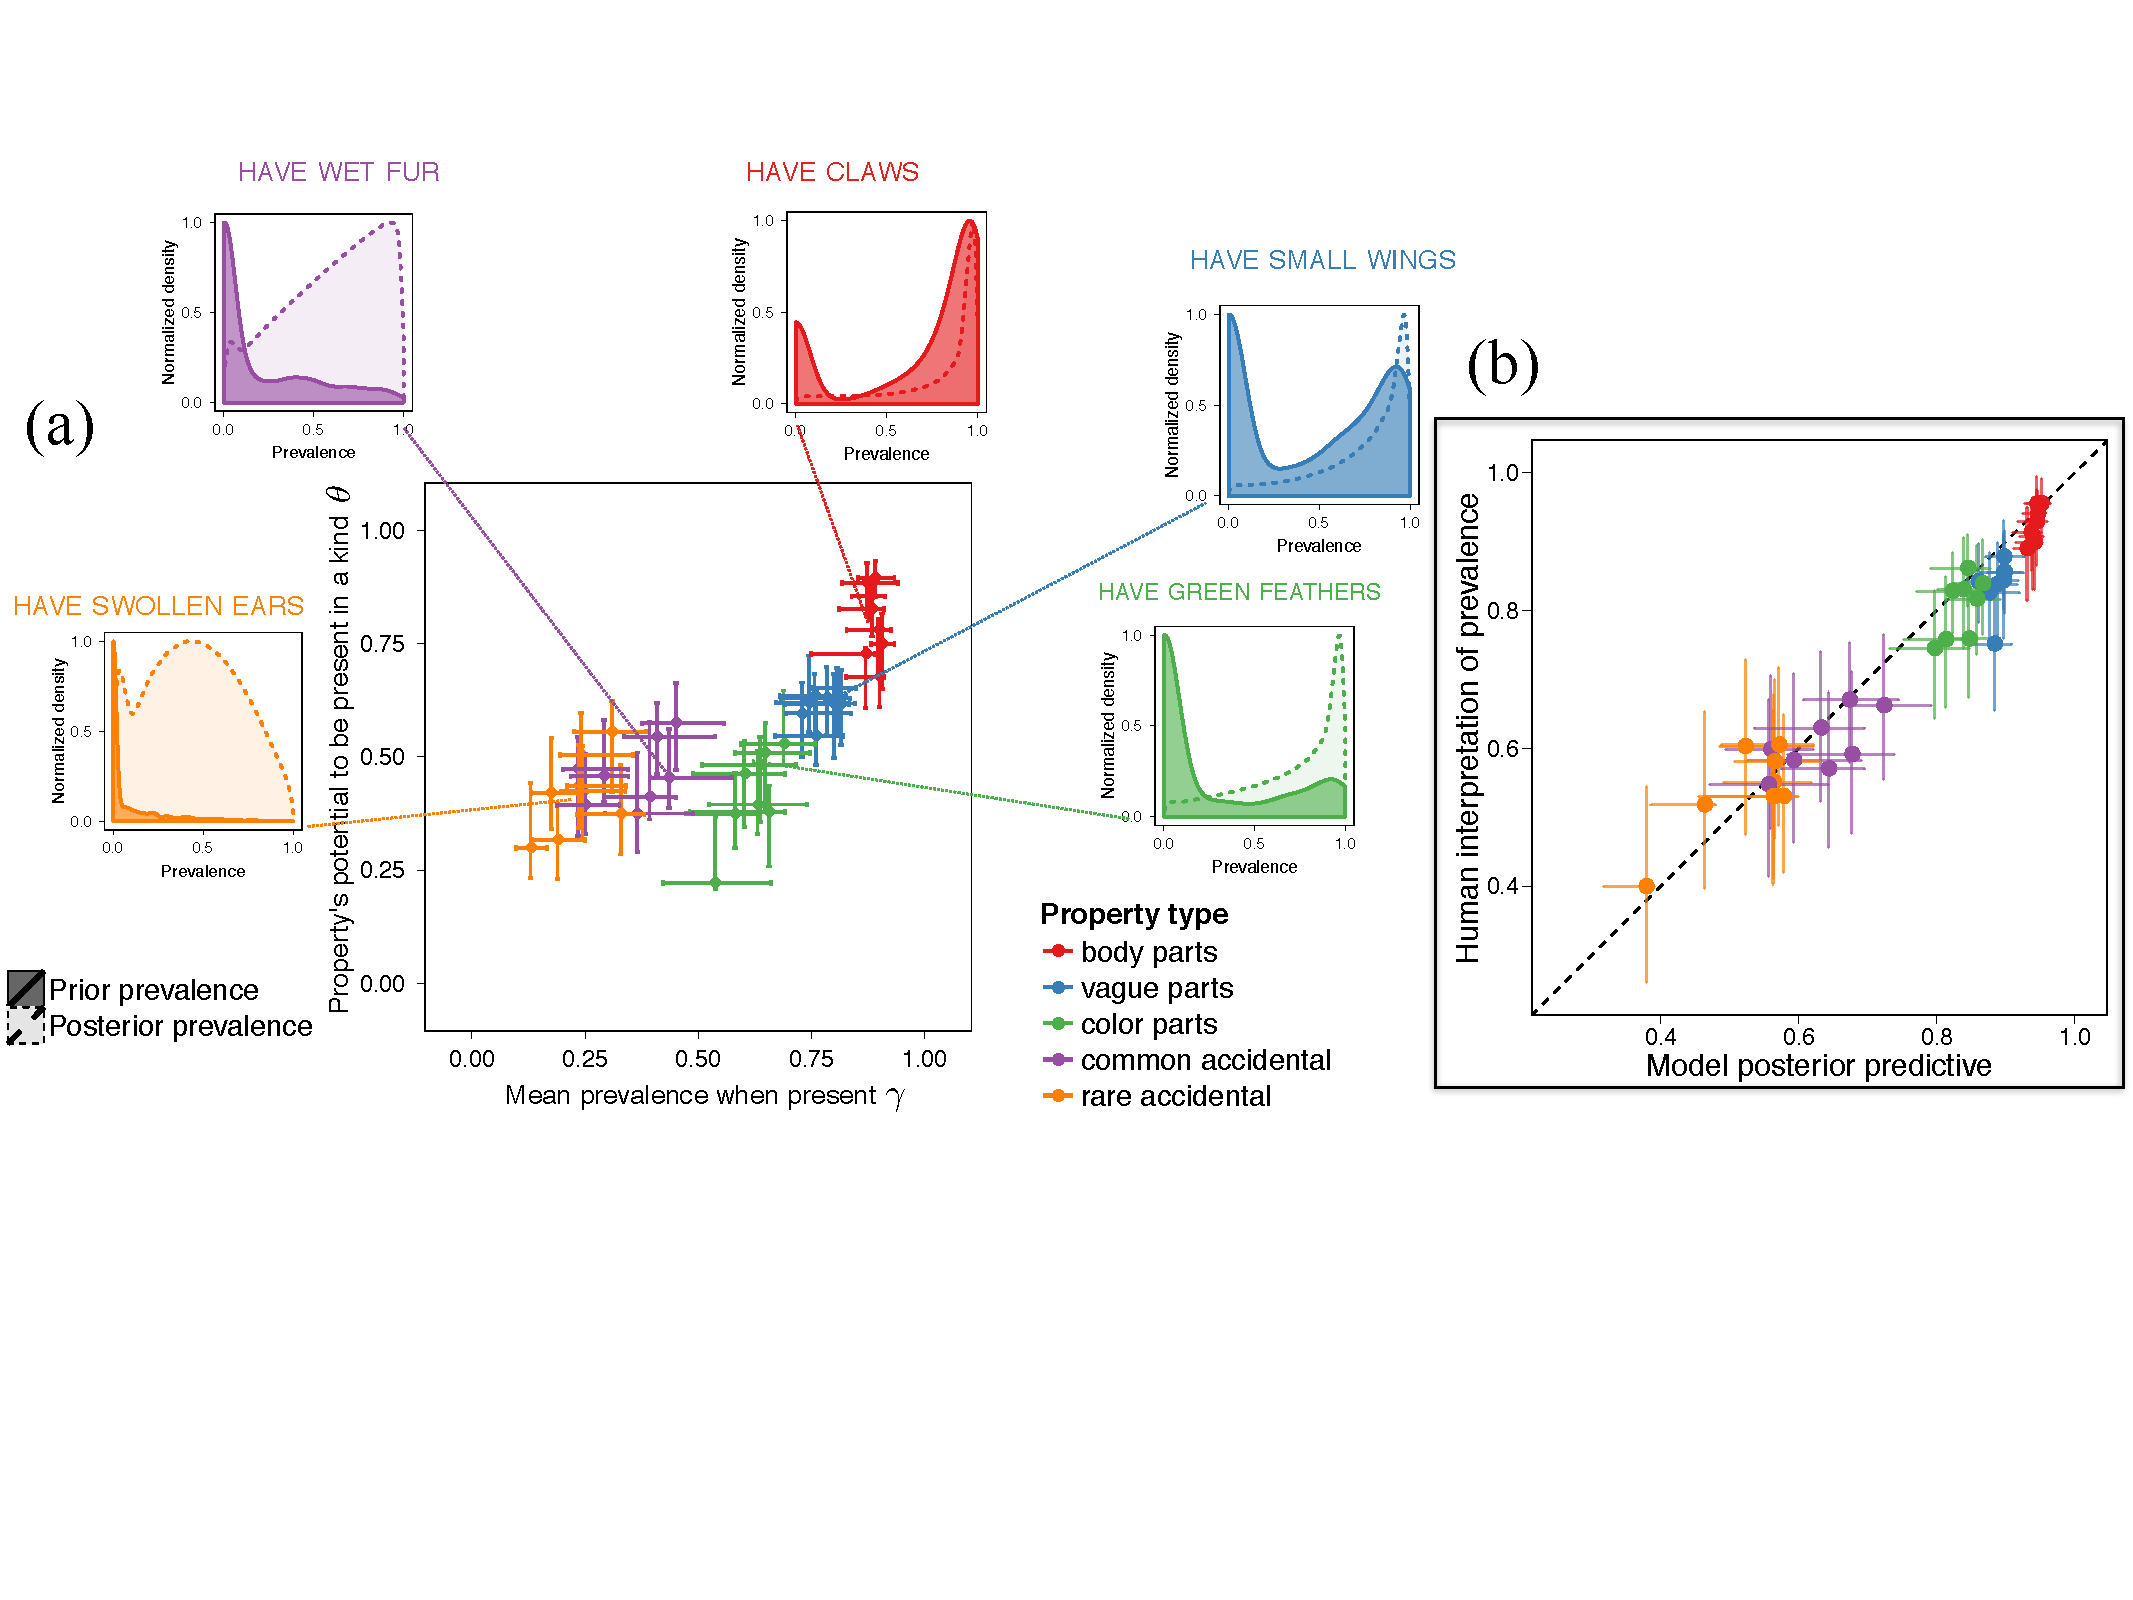
\includegraphics[width=\columnwidth]{prevalence-implied-wPriors}
    \caption{(a) Prevalence prior distributions empirically elicited for 40 animal properties.
    Parameters of the structured statistical model---$\phi$ and $\gamma$---reveal quantitative differences in beliefs about the prevalence of conceptually different types of properties (scatterplot). 
    Inset plots show differences in shapes between biological properties (red, green, blue; bimodal) and accidental properties (orange, purple; unimodal).   
  These differences give rise to the variability of interpretations of generic utterances.
  (b)
  Human interpretation of prevalence upon hearing a generic compared with the $L_1$ model posterior predictive. 
    Participants and the model interpret generics differently for different property types: Generics of biological properties (red, blue, green) have  strong interpretations while generics of accidental properties (purple, orange) are weaker. 
      Error bars denote Bayesian 95\% credible intervals.
  }
  \label{fig:prior2}
\end{figure*}




\section*{Experiment 2b: Interpretations of novel generics}

Our model of generic interpretation, the pragmatic listener model $L_1$ (Eq.~\ref{eq:L1}), predicts that the interpretations of generics in terms of prevalence should vary as a function of the prevalence prior.
Here, we test the degree to which the predictions based on the empirically elicited prevalence priors for 40 items (from Expt.~2a) match human judgments of how the widespread the property is upon hearing a generic.

%We tested the degree to which the $L_1$ listener model, Eq.~\ref{eq:L1}, coupled with the empirically-elicited priors, $P(x)$, from Expt.~2a predicted the interpretation of a generic sentence consisting of a novel category with one of the forty properties described above.
%degree to which the generic implied the property was widespread in the kind. 

%The full cover story is described in {\it SI Section C} and is the same for Expt.~2c.
%The original study by \citeauthor{Cimpian2010} found a difference in the implied prevalence between ``color parts'' (e.g. \textsc{yellow fur}) and accidental properties (e.g. \textsc{wet fur}).
%The prevalence priors inferred from Expt.~2a suggest that generic interpretation could be even more variable.
%For this reason, we included three types of biological properties: parts (e.g. \textsc{fur}), color--part pairs (e.g. \textsc{yellow fur}) and gradable adjective--part pairs (e.g. \textsc{curly fur}). 
%We also coded the accidental properties from Expt.~2a as either ``common'' or ``rare'' using a by-item median split based on \emph{a priori} expected prevalence when present.
%Most of the materials we used were from \citeauthor{Cimpian2010}. 
%The materials used were 30 novel animal categories (e.g. lorches, morseths, blins) each paired with a unique property. 
%Biological properties were made by pairing a color with a body-part (e.g. purple feathers, orange tails). 
%Accidental properties used the same set of body-parts but modified it with an adjective describing an accidental or disease state (e.g. broken legs, wet fur). 
%Each participant saw a random subset of 10 unique animal-property pairs for each type of property (biological and accidental). 


\subsection*{Method}

\subsubsection*{Participants}

We recruited 40 participants over MTurk to determine how widespread different properties are believed to be upon hearing a novel generic.  
The experimental design is very similar to \citeA{Cimpian2010}, and we chose to have a sample size at least twice as large as the original study (original n=15). 
%This is a quantitative experiment with only quantitative comparisons planned.
%Participants were restricted to those with US IP addresses and with at least a 95\% MTurk work approval rating. 
All participants were native English speakers. 
The experiment took about 5 minutes and participants were compensated \$0.60.

\subsubsection*{Procedure and materials}

In order to get participants motivated to reason about novel kinds, they were told they were the resident zoologist of a team of scientists on a recently discovered island with many unknown animals; their task was to provide their expert opinion on questions about these animals.
Participants were supplied with the generic (e.g. ``Feps have yellow fur.'') and asked to judge prevalence: ``What percentage of feps do you think have yellow fur?''. 
Participants completed in randomized order 25 trials: 5 for each of the biological properties and 10 for the accidental (described in Expt.~2a).
The experiment in full can be viewed at \url{http://stanford.edu/~mtessler/generics/experiments/asymmetry/asymmetry-2.html}. 

\subsection*{Analysis and results}

The pragmatic listener $L_1$ model provides posterior beliefs about prevalence, given prior beliefs and a generic utterance.
This model has one parameter governing the optimality of the hypothetical speaker $S_1$ in Eq.~2. 
We put the same uninformative prior over this parameter as previously: $\lambda_1 \sim \text{Uniform}(0, 20)$.
We learned about the parameter's \emph{a posteriori} credible values by running 3 MCMC chains of 100,000 samples (removing 50,000 for burn-in) using the Metropolis-Hastings algorithm.
The MAP and 95\% credible interval for $\lambda_1$ are 14.8 [6.4, 19.9].

We look at the posterior predictive distribution of $L_1$, integrating out the model parameter.
We first explore two important trends predicted by the pragmatic listener model.
In Figure \ref{fig:exp2b}, solid lines, we see the implied prevalence judgments are predicted (at the property class level) to vary linearly with the \emph{a proiri} expected prevalence. 
A mixed-effects linear model with random by-participant effects of intercept and slope indeed reveals the more prevalent a property is expected to be \emph{a priori}, the stronger the implications of a generic statement ($\beta = 0.57; SE = 0.08; t(39) = 7.12; p < 0.001$).
The prevalence implied by a generic is also predicted to be greater than the \emph{a proiri} expected prevalence.
A mixed-effects linear model with random by-participant effects of intercept and random by-item effects of intercept and condition reveals implied prevalence after hearing a generic is significantly greater than the \emph{a priori} prevalence ($\beta = 0.17; SE = 0.018; t(39) = 9.7; d = 0.64; p < 0.001$).
%The generic thus does more than simply signal the category has the property; it carries with it the communicative weight of a speech-act, and implies a prevalence even higher than one would infer just by generalizing based on instances.
As for the quantitative accuracy of the model, on a by-item level, the pragmatic listener model predictions closely align with the human judgments of prevalence for novel generics ($r^2(40)=0.94$, MSE=0.002).
Human participants and our model display the same sensitivity of generic interpretation to details of the property (Figure \ref{fig:prior2}b). 
We now have strong support for both of the major predictive components of our model: generic endorsement, modeled as a speaker $S_2$, and generic interpretation, modeled as a listener $L_1$.

%\mht{I'm a little unsure what the order of this should be right. Right now: linear effect of a priori prevalence; implied prevalence > a priori prevalence; pragmatics model predictions}

%\ndg{i don't really understand this paragraph...}
%To understand more fully how the model makes these predictions, we performed two exploratory analyses to test whether or not:
%(1) implied prevalence judgments varied linearly with the \emph{a proiri} expected prevalence;
%and (2) the prevalence implied by a generic is greater than the \emph{a proiri} expected prevalence.
%Both exploratory analysis returned confirmatory evidence. 
%A mixed-effects linear model with random by-participant effects of intercept and slope reveals the more widespread a property is expected to be \emph{a priori}, the stronger the implications of a generic statement ($\beta = 0.57; SE = 0.08; t(39) = 7.12; p < 0.001$, providing evidence for (1).
%A mixed-effects linear model with random by-participant effects of intercept and random by-item effects of intercept and condition reveals implied prevalence after hearing a generic is significantly greater than the \emph{a priori} prevalence ($\beta = 0.17; SE = 0.018; t(39) = 9.7; d = 0.64; p < 0.001$), providing evidence for (2).
%The generic does more than simply signal the category has the property; it carries with it the communicative weight of a speech-act, and implies a prevalence even higher than one would infer just by generalizing based on instances.


% We subjected the human prevalence judgments to a mixed-effects 
%
%Human prevalence judgments after reading the generic were affected by the type of property and its corresponding mean prevalence when present )\footnote{These statistics are the result of a mixed-effects linear regression with a maximal mixed-effect structure: Random by-participant effects of intercept and slope}. 
%We compared participants judgments to interpretations of the pragmatic listener $L_1$ (Eq.~\ref{eq:L1})) about the likely prevalence of the property after hearing a generic about an unfamiliar kind (e.g. \emph{Lorches have green feathers.}). 

%, in the same spirit as \cite{Gelman2002}. 



%The pragmatic listener in Eq.~\ref{eq:L1} is sensitive to the property in question and its corresponding distribution on prevalence.
%type of property (and its corresponding prior distribution on prevalence) when interpreting a novel generic.





%Particularly, the \emph{a priori} mean conditional prevalence will guide interpretation as it describes the distribution assuming the property is present. \ndg{why?}
%Again, $P(x)$ was measured empirically ($n=40$, see Supplement Section C).
%The five property types fell on a continuum of \emph{a priori} mean conditional prevalence (Figure \ref{fig:prior2}; x-axis). 
%Biological properties are expected \emph{a piori} to be more prevalent within a kind than accidental properties, with fine-grained differences even among types of biological and accidental properties.
%For instance, within a given kind, colored body parts (e.g. \textsc{green wings}) are expected \emph{a priori} to be less prevalent than some gradable adjectives (e.g. \textsc{small wings}). 
%Some accidental properties are expected to be relatively more prevalent \emph{a priori} than others (``common accidental'' vs. ``rare accidental''; e.g. \textsc{wet fur} vs. \textsc{broken legs}; Figure \ref{fig:prior2}, orange and purple plots).

%These distributions are not necessarily peaked at 100\%, and the expected 
%Figure \ref{fig:prior2} (right) shows the region of interest of these distributions by removing the mass at 0. %
%With the exception of the body part category, properties are mostly likely to be absent from the category (Figure \ref{fig:prior2} left; modes of distributions are at 0).
%If the property is present in the category, the most likely prevalence for biological properties (``part'', ``color part'', and ``vague part'') is 100\% (Figure \ref{fig:prior2} right; modes of blue, green, and red distributions are at 1).
%This is not the case with the prevalence priors for accidental properties, for which lower values are more likely (Figure \ref{fig:prior2} right; modes of orange and purples distributions are at some low prevalence).
%\ndg{this analysis has gotten a lot less transparent since i looked last. it's not at all clear why we should care about the gradient against "some". }
%
%However, the generic does more than merely inform a listener that the property is present: 
%A generic carries the communicative force of a speech act, and thus implies the property is \emph{more prevalent} than a listener would expect (Figure \ref{fig:exp2b} solid line lies above $y=x$ line).
%\ndg{i think if we're going to rely on it we need to set this contrast up much more clearly earlier: many properties are never present in most categories. at the least, the generic rules out the absence of the property (ie ``some''). we want to test whether it is stronger than some. -- though really?}
%The listener model (Eq.~\ref{eq:L1}) produced the same strong interpretation along a gradient (Figure \ref{fig:exp2b}, Right, solid line), displaying the sensitivity to abstract beliefs about the properties that human participants show. 
%We performed a by-item analysis comparing the implied prevalence data to model predictions and found a good quantitative fit ($r^2(40) = 0.89$; see Supplement Section D5). 
%\ndg{
%Generics ``once accepted [...] appear to be commonly taken in a rather strong sense, as if the qualifier \emph{always} had implicitly crept into their interpretation'' (\cite{Abelson1966}, Cf.~\cite{Cimpian2010}). 
%\cite{Gelman2002} found that adults interpret novel generic statements about familiar kinds (e.g. \emph{Bears like to eat ants.}) as implying that almost all of the category have the property (e.g. almost all bears like to eat ants).
%Why is generic language interpreted so strongly if the criterion for endorsement is so flexible? 
%}

\section*{Experiment 2c: The asymmetry between truth conditions and interpretations} 


There is a surprising d\'{e}colage between the truth conditions and interpretations of generic language: Interpretations are often strong while truth conditions are flexible. 
Generic statements (e.g. \emph{Glippets have yellow fur.}) thus show an asymmetry between their \emph{truth conditions} and the prevalence implied by the statement; this is in contrast to the behavior of quantifiers statements involving ``all'' or ``most'' \cite{Cimpian2010}. 
Upon reading a generic, participants infer that the property is widespread (e.g. almost all glippets have yellow fur): \emph{implied prevalence} is near ceiling.
By contrast, using a truth judgment task, participants endorsed generics for a much wider range of prevalence levels (e.g. even when ``30\% of glippets have yellow fur.''). 
However, this mismatch between \emph{truth conditions} and \emph{implied prevalence} is significantly reduced for generics of properties plausibly construed as accidental (e.g. \emph{Glippets have wet fur.}).
\ndg{this paragraph needs editing for flow.}

%Because generics get judged ``true'' at almost all prevalence levels, the average prevalence to yield a ``true'' response is substantially less than the average prevalence inferred upon hearing a generic (which is near ceiling). 

Below we replicate the basic asymmetry findings of \citeA{Cimpian2010} and discover even more variability in the mismatch between \emph{truth conditions} and \emph{implied prevalence} using the expanded stimulus set from Expt.~2a.
In addition, we now test both our models (generic endorsement [speaker $S_2$] and generic interpretation [listener $L_1$]) in the same experimental paradigm. %models predicts the asymmetry and the context-sensitivity of this phenomenon.

%Expt.~2b revealed how generics imply the property is more widespread than what would be expected \emph{a priori}. 
%Comparing to the average prevalence required to assent is another way to explore how generics exaggerate the evidence. 

\subsection*{Method}

We re-analyze the data from Expt.~2b as the \emph{implied prevalence} data.
The following paradigm is to measure the corresponding \emph{truth conditions}.

\subsubsection*{Participants}

We recruited 40 participants over MTurk.  
%We chose a sample size at least twice as large as the original study by \citeA{Cimpian2010} (original n=20), and to match Expt.~2b. 
All participants were native English speakers. 
None of the participants completed Expt.~2b (interpretations of novel generics).
The experiment took about 5 minutes and participants were compensated \$0.60.

\subsubsection*{Procedure and materials}

The cover story and materials were the same as in Expt.~2b.
On each trial, participants were given a statement about a property's prevalence within a novel kind (e.g. \emph{50\% of feps have yellow fur.}). Participants were then asked whether or not they agreed or disagreed with the corresponding generic sentence (e.g. \emph{Feps have yellow fur.}). Prevalence varied between 10, 30, 50, 70, and 90\%.

The experiment consisted of 25 trials: 5 trials for each of 5 types of properties measured in Expt.~2a (part, color part, vague part, common accidental, rare accidental). 
Each prevalence level appeared once for each property type (5 prevalence levels x 5 property types). 

\subsection*{Analysis and results}

For both behavioral data and model predictions (Eq.~\ref{eq:S2}) we computed the average prevalence that led to an assenting judgment (the \emph{average prevalence score}), for each property type and participant, following the procedure used by \citeA{Cimpian2010}.
For example, if a participant agreed with the generic whenever the prevalence was 70\% or 90\% and disagreed at the other prevalence levels, that participant received an \emph{average prevalence score} of 80\%.

For our pair of models, there are two parameters (the two speaker optimality parameters).
We infer them using the same Bayesian data analytic approach as before. 
The MAP and 95\% HPD intervals for $\lambda_1$ is 19.5 [10.5, 19.9] and $\lambda_2$ is 0.4 [0.34, 0.49].
We then subjected the generic endorsement model to the same procedure as the human data. % subjected our model to the same procedure. 
%
The speaker model $S_2$ returns a posterior probability of producing the generic, for each level of prevalence\footnote{We assume here that the prevalence told to the participant is the subjective probability that that speaker $S_2$ is trying to communicate. In some situations this assumption may be invalid due to theory-driven considerations on behalf of the speaker. For example, if the participant believes the prevalence being reported in the experiment is describing a temporary or accidental state and not one that is likely to be predictive of the future prevalence, the speaker may derive a subjective probability substantially less than that stated verbally in the experimental prompt.}. 
We sample a response (\emph{agree} / \emph{disagree}) from this posterior distribution for each prevalence level, simulating a single subject's data.
As with the human data, we took the trials where the model agreed with the generic, and took the mean of the prevalence levels corresponding to those trials, giving us the average prevalence at which the model assented to the generic.
We repeated this for each type of property 40 times to simulate a sample of 40 participants. 
We repeated this procedure 1000 times to bootstrap 95\% confidence intervals.

The generic endorsement model (speaker $S_2$) predicted that \emph{average truth conditions} should not vary appreciably across the different types of properties, consistent with the fact that generics are acceptable for broad range of prevalence levels for all property types.
A similar absence of a gradient was observed in the human data ($\beta = 2.82; SE = 4.02; t(39) = 0.70; p = 0.49$; Figure \ref{fig:exp2b}, dotted lines). 
Interpretations of generic utterances are stronger than their average truth conditions for the biological properties but not for the accidental properties (Figure \ref{fig:exp2b}) with both human data, replicating \citeA{Cimpian2010}, and the model; the extent of the difference is governed by prior property knowledge (mean prevalence when present $\gamma$, from Expt.~2a).
The listener and speaker pair of models predicts human endorsements and interpretations of novel generic utterances well ($r^2(10) = 0.87$, MSE = 0.008).
Thus, our model predicts that the asymmetry between truth conditions and implied prevalence should hold, but only for properties with the most extreme prior beliefs.

\ndg{i don't think the overall logic of this paragraph, connecting $\lambda_2$ to theoretical mismatch, will be clear to readers. explain better?}
Having corroborated the model with empirical data, we again examine the model more closely.
The $\lambda_2$ parameter, which is only used to model the truth judgments task, is credibly below 1: participants' behavior is slightly more random than veridical Bayesian updating according to our model.
Our $S_2$ model predictions assume that the prevalence that the speaker model is aiming to communicate is, in fact, the prevalence told to the participant in the experimental prompt.
However, if participants' beliefs about properties are inconsistent with the prevalence statement they are given (e.g., 90\% of lorches have broken legs), they may believe the current prevalence is aberrational, and assign a truth judgment to the generic based on theory-derived considerations (e.g., that in the future, fewer than 90\% of lorches will have broken legs).
If this is so, we would predict that the $\lambda_2$ parameter would be lowest for properties that are unlikely to be present at all prevalence levels given in the experiment.
We predict this would be the case for the accidental properties (which are unlikely to be present in high prevalence) and the body part properties (which are unlikely to be present in low prevalence; e.g. 10\% of lorches have wings).
To investigate this, we implemented a model where the $\lambda_2$ parameter was allowed to vary by item-type.
The posterior distributions over $\lambda_2$ are shown in Appendix Figure \ref{fig:asymmetry-params-byItem} \ndg{this fig isn't that useful}.
Indeed, we found that the $\lambda_2$ parameter is lowest for the rare accidental properties (HPD = [0.03, 0.24]), followed by the common accidental properties (HPD = [0.27, 0.60]) and then the body part properties (HPD = [0.33, 0.76]).
For the colored and vaguely described body parts, the speaker optimality parameters were considerably higher (color HPD = [0.50, 0.99]; vague HPD = [0.72, 1.32]).
This suggests that there is more to communicating generalizations than conveying the current frequency. % evidence is interpreted through the lens of theoretical considerations, and that has important implications for generic truth conditions.
But what is prevalence if not the current frequency?
%In our final experiment, we develop a paradigm for testing this idea.


%
%\begin{figure}
%\centering
%    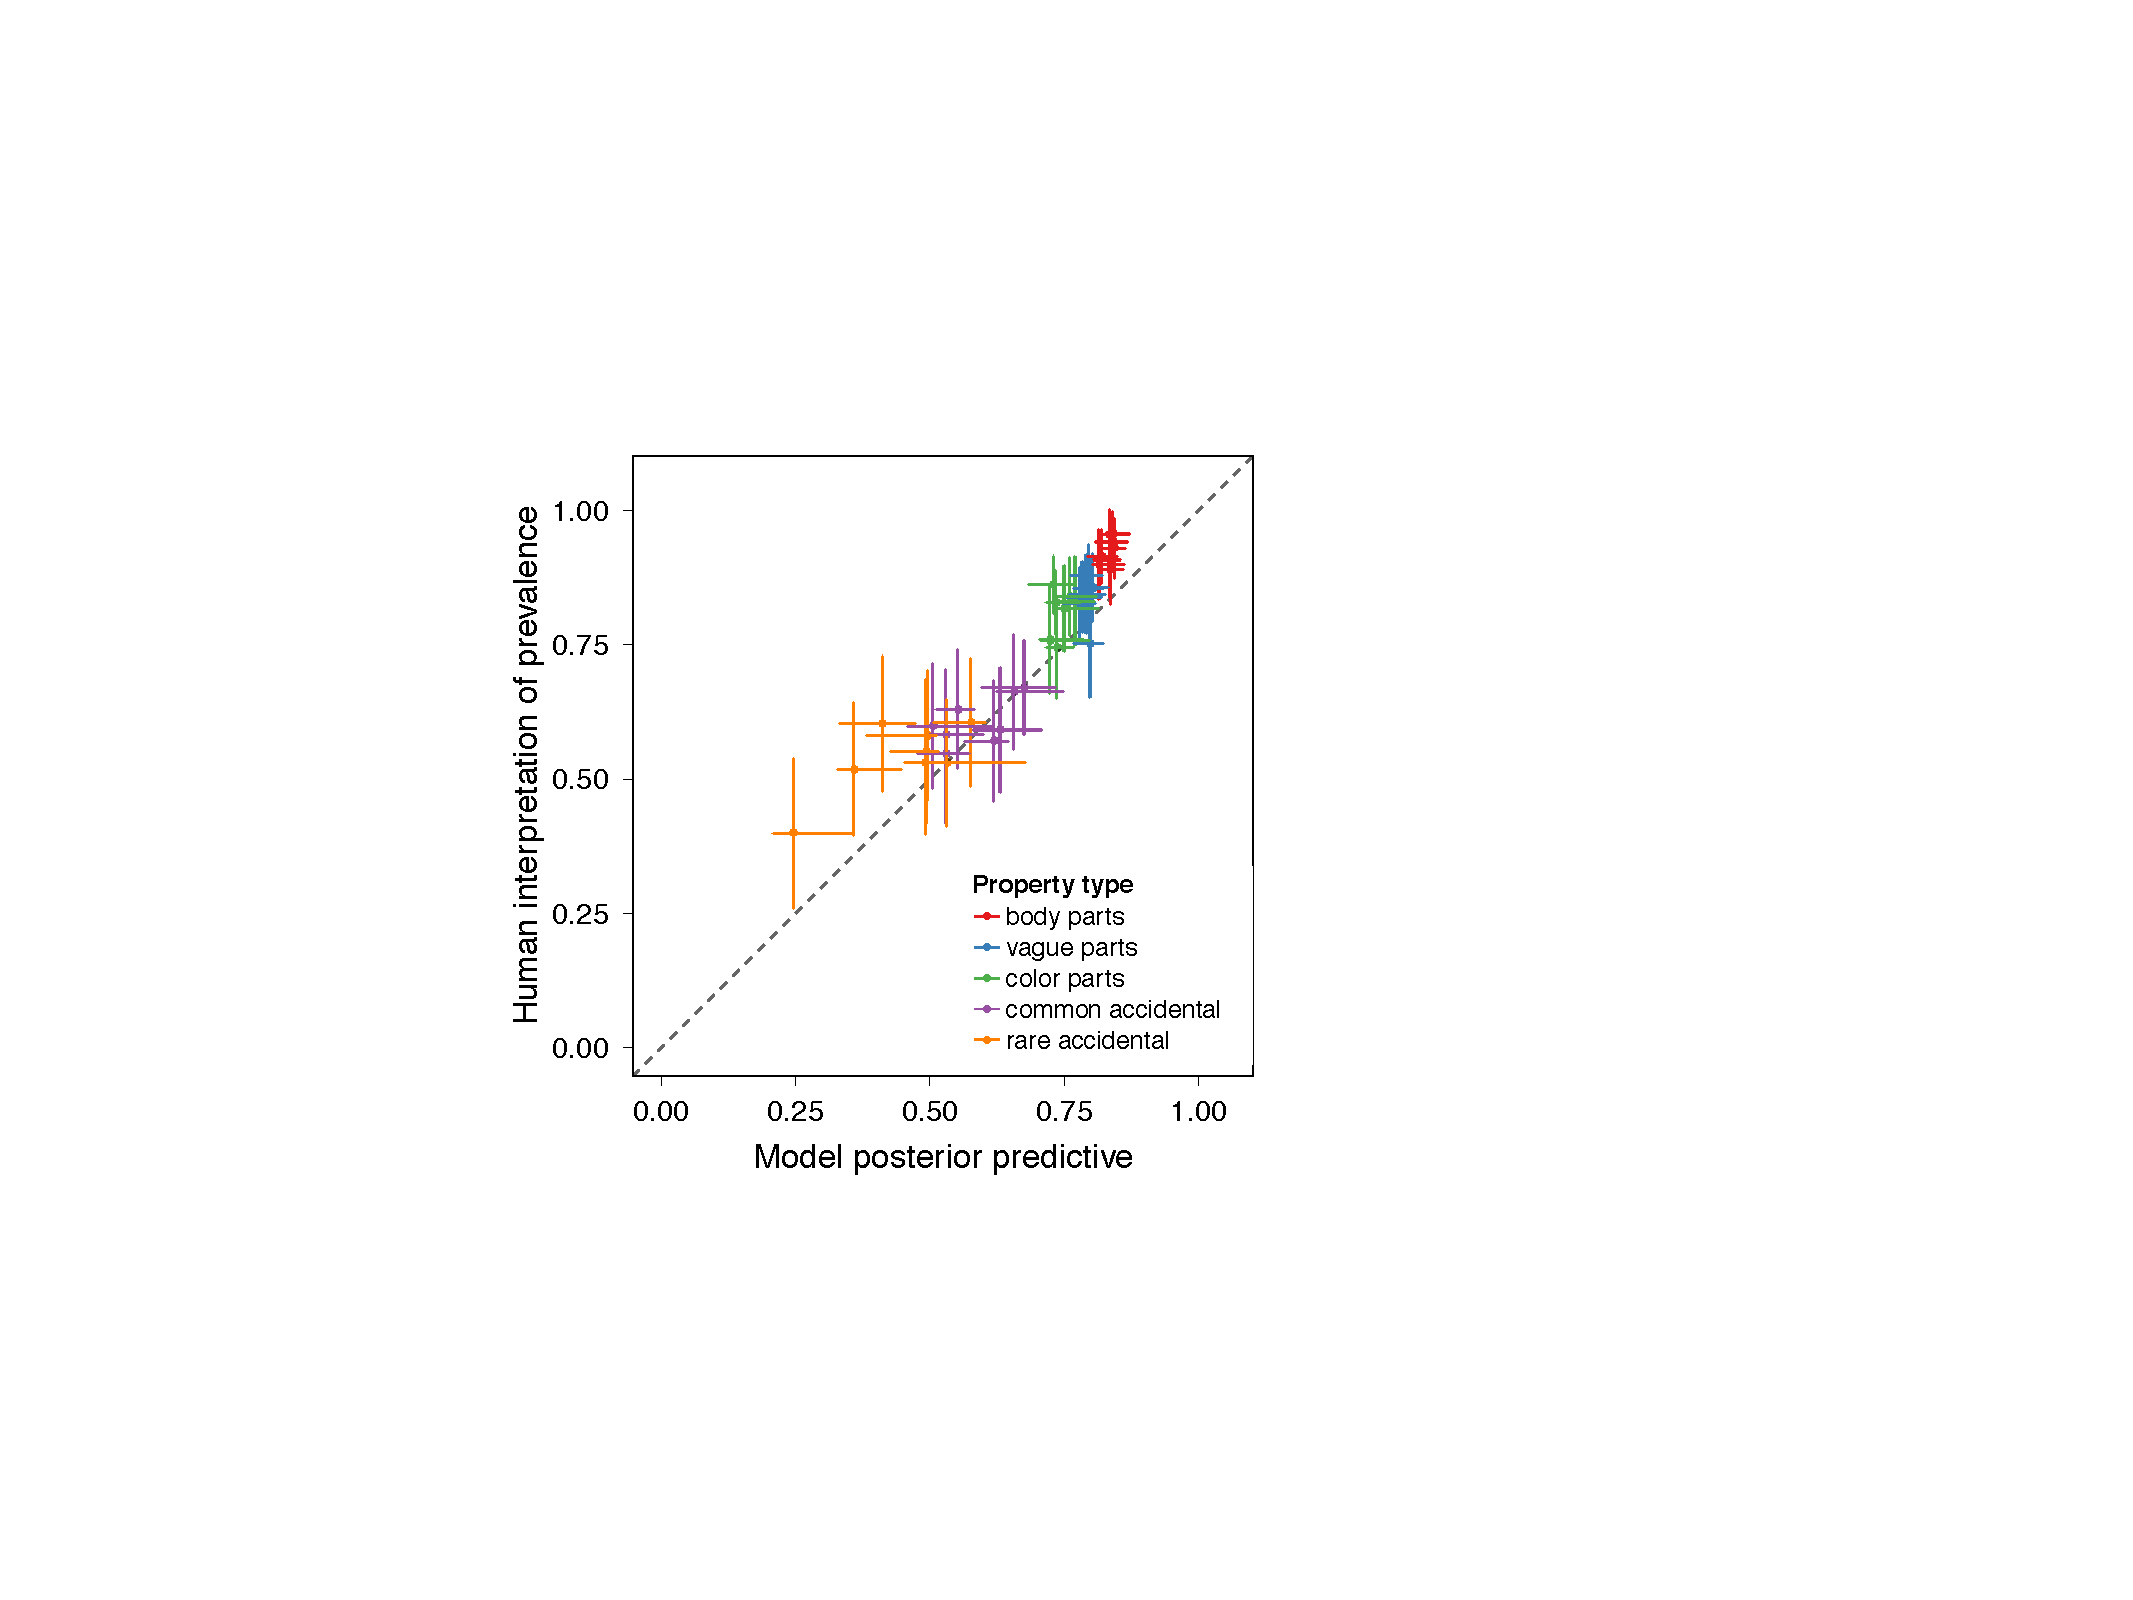
\includegraphics[width=0.5\columnwidth]{implied-byItem-mh100kX2b.pdf}
%    \caption{Human interpretation of prevalence upon hearing a generic compared with the $L_1$ model posterior predictive. 
%    Participants and the model interpret generics differently for different property types: Generics of biological properties (red, blue, green) have  strong interpretations while generics of accidental properties (purple, orange) are weak.}
%    %    Error bars denote bootstrapped 95\% confidence intervals for the data and Bayesian 95\% credible intervals for the model.}
%  \label{fig:impliedByItem}
%\end{figure}

%Interestingly, we observe greater implied prevalence of common accidental properties than rare accidental properties, given our median split based on the prior elicitation task ($\beta=0.061; SE = 0.025; t(39) = 2.47; p = 0.018$) \footnote{These statistics are the result of a mixed-effects linear regression with a maximal mixed-effect structure: Random by-participant effects of intercept and slope}.
%Implications of generics of body parts was significantly greater than those of the biological properties used by \cite{Cimpian2010} (here, ``color parts'') ($\beta=0.118; SE = 0.024; t(39) = 4.74; p < 0.001$). 
%There was also a trending effect for the implications of vague body parts (e.g. curly fur) to be greater than those of color parts (e.g. yellow fur) ($\beta=0.032; SE = 0.016, t(54.8) = 1.95; p = 0.056$), possibly due to the belief that the same kind of animal can come in many different colors (e.g. dogs).
\begin{figure*}
\centering
    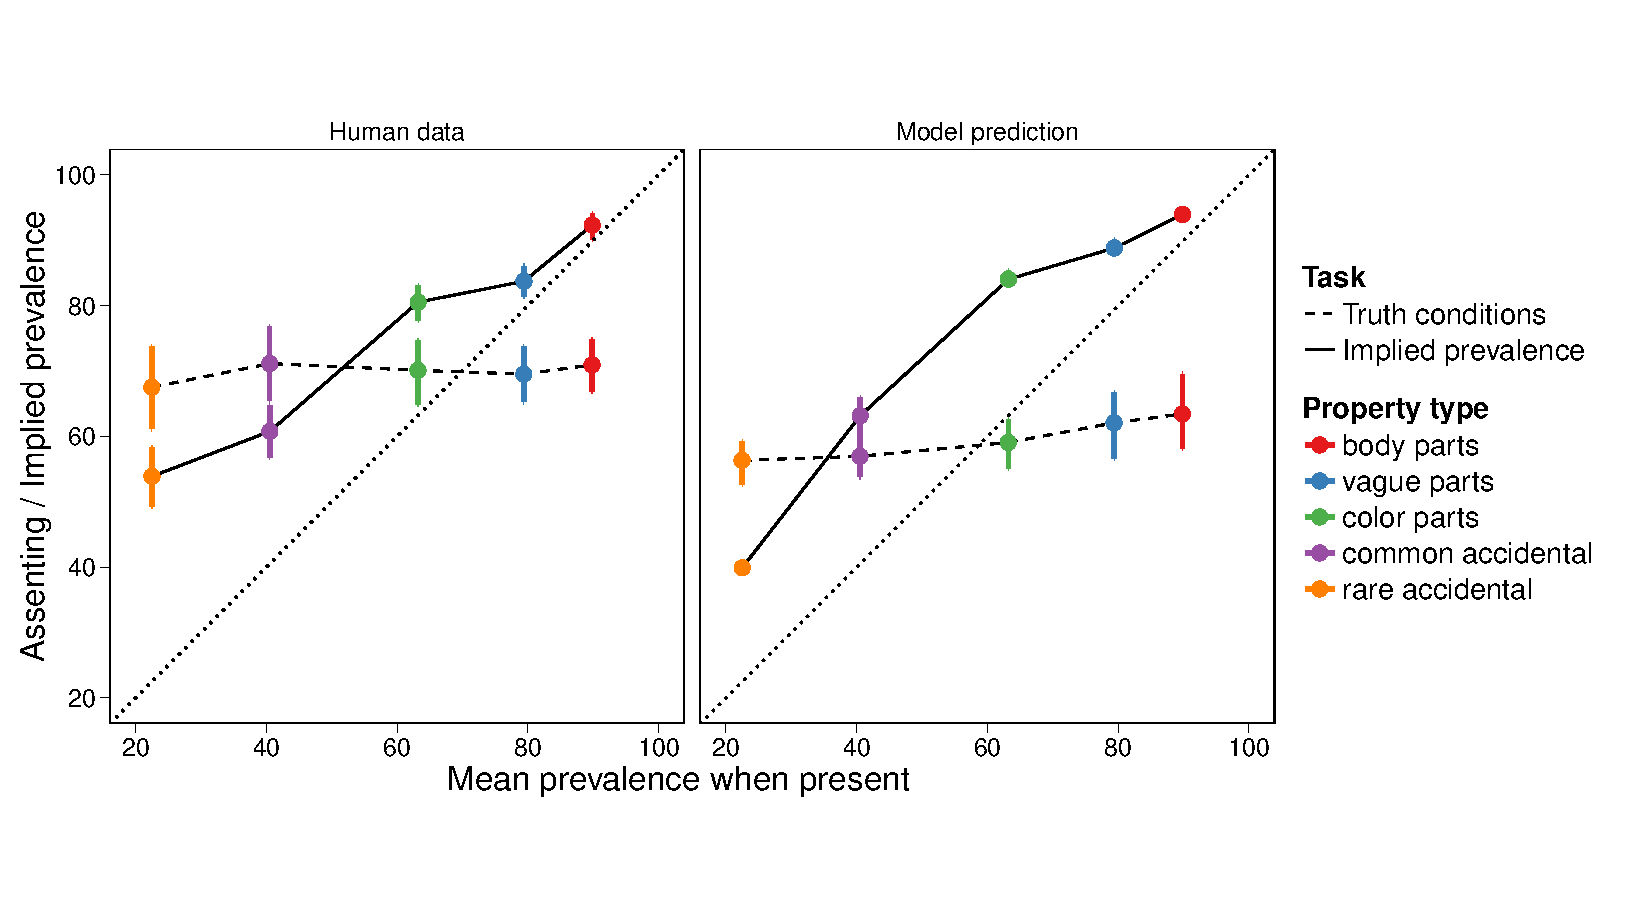
\includegraphics[width=\columnwidth]{unfamiliar-asymmetry-predictive-data.pdf}
%    \includegraphics[width=1.2\columnwidth]{asym-lines-data-model.pdf}
    \caption{Human judgments and model predictions of prevalence implied by novel generic utterances (implied prevalence task; solid line) and average prevalence that leads to an acceptable generic utterance (truth conditions task; dotted line) as it relates to the \emph{a priori} mean prevalence when present $\gamma$.
    Expectations of prevalence are higher after hearing a generic than before hearing it (solid line compared to $y=x$ line; both for human data and model).
    %$y = x$ line denotes the prevalence inferred upon knowing the property is prettyesent in the kind. 
    %For each kind of property, the generic utterance implies a higher than expected prevalence.
    Generic statements about biological properties, imply that the property is widespread in the category, for both human participants and the model (solid line: red, blue and green). 
    Generics about accidental properties do not result in such a high implied prevalence (solid line: purple and orange).  
	While the implications of generic utterances are highly variable across the different types of properties, the average prevalence that leads to an acceptable generic does not vary, for participants or the model.
        %Generic statements are accepted for a range of prevalences, resulting in a intermediate average prevalence (dotted line) that deoesn't vary by property type for the truth conditions task. 
%    Error bars denote bootstrapped 95\% confidence intervals for the data and Bayesian 95\% credible intervals for the model.
%    \ndg{change x-axis label to "a priori expected prevalence" or something like that -- "within-category prevalence" is ambiguous.}
}
  \label{fig:exp2b}
\end{figure*}


%Consistent with the effects reported by \cite{Cimpian2010}, biological properties (body, vague, and color parts) have stronger interpretations than their truth conditions would suggest (Figure \ref{fig:exp2b}; solid vs. dotted lines; green, blue and red points), whereas accidental properties receive more modest interpretations (orange and purple points).



%How does the model capture these fine-grained inferences that listeners draw?
%Consider again the belief distributions about the properties inferred from Expt.~2a (Figure \ref{fig:prior2}). 
%All of the properties have substantial mass at 0 (Figure \ref{fig:prior2} Left). 
%This gives the speaker validity in saying the generic at low prevalence levels (though the speaker's confidence in doing so increases as prevalence increases).
%The listener has the complementary task: She brings \emph{a priori} uncertainty about the generic threshold to the table.
%Consider what would happen if she inferred the most conservative threshold (0) and responded with the \emph{maximum a posteriori} (MAP) of the distribution. 
%A threshold of 0 produces Figure \ref{fig:prior2} (right), because it only rules out the possibility that 0\% of the category has the property. 
%The resulting peaks (MAPs) of the distributions are near 1 for biological properties (parts, color parts, vague parts) and around 10\% for accidental properties (both rare and common). This alone would produce variable interpretations. 
%Our listener, however, does something wiser: She integrates over her uncertainty about the threshold (believing the speaker to be not just truthful but informative as well), and produces interpretations that both take reflect the whole distribution.
%This results in subtle differences between the implications of body parts (e.g. ``Lorches have wings.'') and  color parts (e.g.``Lorches have purple wings.''), and differences in interpretations of rare and common accidental properties. 
%

\section*{Prevalence is a predictive probability}

So far, we have shown that property prevalence is sufficient to formalize the semantics of generic statements as an underspecified scalar denotation.
But what is property prevalence?
If generic language is truly conveying generalizations, it would be useful for it to reflect expectations, not just the current statistics in the world.
The current frequency of a property is often a good indicator of future frequency, yet statistics can be distorted by spurious events.
The causal history of a property may be more or less important for implying the property will be present in future situations.
Does generic language communicate prevalence in terms of past frequency or future expectations?

To answer this, we adopt an experimental paradigm used by \citeA{Gelman2007} to show that generic language is sensitive to theory-based considerations.
In the original paradigm, participants are told a story about a novel creature (e.g. \emph{dobles}) and a property of that kind (e.g., \emph{having claws}).
Participants are then either told that the creature is born with the property or that it acquires the property through extrinsic means (e.g., by finding claws and putting them on). 
Then, participants are told about an event that either causes the property to disappear (e.g., they drank a chemical and their claws fell off) or that leaves the property intact, and are asked whether or not the generic (e.g. \emph{Dobles have claws}) applies.
Adult judgments in this paradigm were sensitive to the origins of the property (i.e. born vs. acquired), and insensitive to the outcome of the event: Participants fully-endorsed the generic when it was inborn, and rejected it when it was acquired.

In Experiment 3a, we use the same basic paradigm to measure \emph{predictive prevalence}: participants' expectations about future instances of the kind.
We explore the predictions of our truth judgments model, assuming that \emph{predictive prevalence} is what is being communicated.
In Experiment 3b, we use a truth judgment task similar to \citeA{Gelman2007} and compare the judgments to the model's predicted endorsements.

\section*{Experiment 3a: Predictive prevalence elicitation}

The design of this experiment is based on a study reported in \citeA{Gelman2007} with some slight modification.
%The original study was done on 14 undergraduates.

\subsection*{Method}

\subsubsection*{Participants}
We recruited 80 participants over MTurk.  
The experiment took about 3 minutes and participants were compensated \$0.35.

\subsubsection*{Procedure and materials}

On each trial, participants read a vignette about a novel creature. For instance,
\begin{quote}
These are dobles. [picture of 10 dobles with claws] Here is how they grew. They grew up with claws. First they were born, then they got bigger, then they were full size. [picture of a doble with claws getting bigger and bigger; in some vignettes, the animal was first shown hatching out of an egg with the relevant property already visible] Then one day they drank a bad chemical. They got very sick and this is how they looked. [10 dobles with no claws]
\end{quote}
The trial proceeded by participants reading the text, and clicking a button to continue to the next part of the story (at which time, the images changed according to the example above).

Participants saw 4 trials: 2 in which the creatures are born with the property, and 2 in which the creatures are shown discovering and acquiring the property (e.g. painting themselves brown).
This was crossed with either the creatures drinking a bad chemical and losing the feature, or drinking a yummy drink and maintaining the feature.
The outcome of this event determined the final screen of images the participant saw (e.g. either 10 dobles with claws or 10 without).

While this final screen was present, we measured \emph{predictive prevalence} by telling participants: ``A new doble was born today. When it becomes full grown, how likely is it that it would have claws?''.
Participants responded using sliders ranging from ``very unlikely'' to ``very likely''.

We used 2 different types of properties: colors (e.g. \emph{Lorches are green.}) and body parts (e.g. \emph{Dobles have claws})\footnote{
For each type of property, there were approximately 8 different exemplars (e.g. different colors, different body parts for different creatures)}.
The creatures were either birds, bugs, or fish, with randomly sampled dimensions.
The experiment in full can be viewed at \url{http://stanford.edu/~mtessler/generics/experiments/predictive/predictive-elicitation-1-elicitation.html}.


\subsubsection*{Results and truth judgment predictions}

The average predicted prevalence for the 4 experimental conditions are shown in Figure \ref{fig:dobles-predictive}(a, top).
We observe a main effect of origins, such that when participants read that the creatures had the property from birth, future creatures  are much more likely to have the property as compared to when the property is acquired.
We see that, in our paradigm, participants are also sensitive to the outcome of the event.\footnote{
It's worth noting that our experiments (Expts.~3a and 3b) differ from the original study by \citeauthor{Gelman2007} in a couple of ways.
In the original study, the first sentence of each vignette used the possessive ``my'': ``These are my dobles.''.
At the end of each vignette, the original study had participants judge two statements in counterbalanced order: ``Do my dobles have claws?'' and ``Do dobles have claws?''
These differences may account for the differences in results.
}
%This is surprising because \citeA{Gelman2007} observed no effect of the event outcome on generic endorsement.
When participants observe a creature who loses the property by drinking a chemical, they report future members of the category are less likely to have the property.
This inference may be driven by beliefs about the property (e.g. the property could be an unstable property if you can lose it simply by drinking something) or by beliefs about the event (e.g. participants may believe this ``chemical drinking'' event is a relatively normal event, and thus it could happen in the future).
Examining the data by item type (color vs. body part), we see this effect is slightly more pronounced for the body parts than the colors (Figure \ref{fig:dobles-predictive}a, bottom). 

We use these predicted probabilities as the prevalence $x$ that the speaker model is trying to communicate: $S_2(u\mid x)$, and examine the model's predicted truth judgments.
For priors $P(x)$, we use the body part and color priors elicited in Expt.~2a.
We see that the model predictions track closely the predicted prevalence, including the subtle by-item difference (Figure \ref{fig:dobles-predictive}b, top and bottom)\footnote{Note that our model's predictions do not deviate substantially from the predicted prevalence because there are only two different priors being used, and the shapes of those distributions do not vary appreciably (see Figure \ref{fig:prior2}).
}.
Thus, we make two novel predictions for generic endorsement in the paradigm by \citeA{Gelman2007}.
We predict that in addition to the main effect of origins, we should see a second main effect of event outcome.
Second, we predict that this effect should be slightly stronger in the case of color properties than in the case of body part properties.

\begin{figure*}
\begin{tabular}{l l}
(a) Elicited predicted prevalence & (b) Truth judgment model predictions\\
\\
\centering
    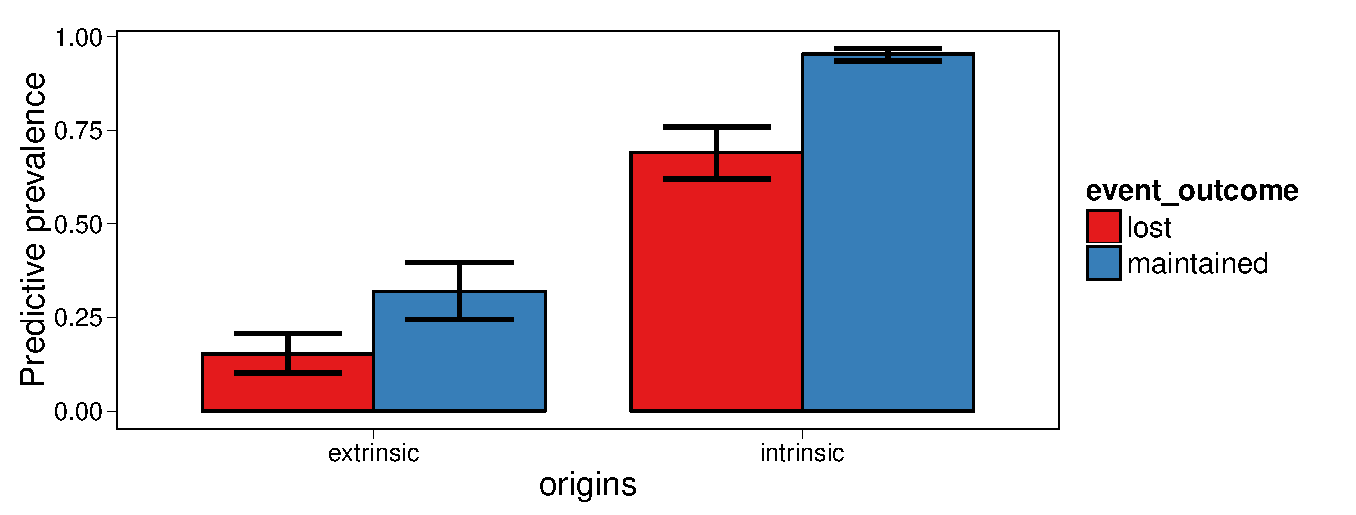
\includegraphics[width=0.5\columnwidth]{dobles-predictive.pdf} &
    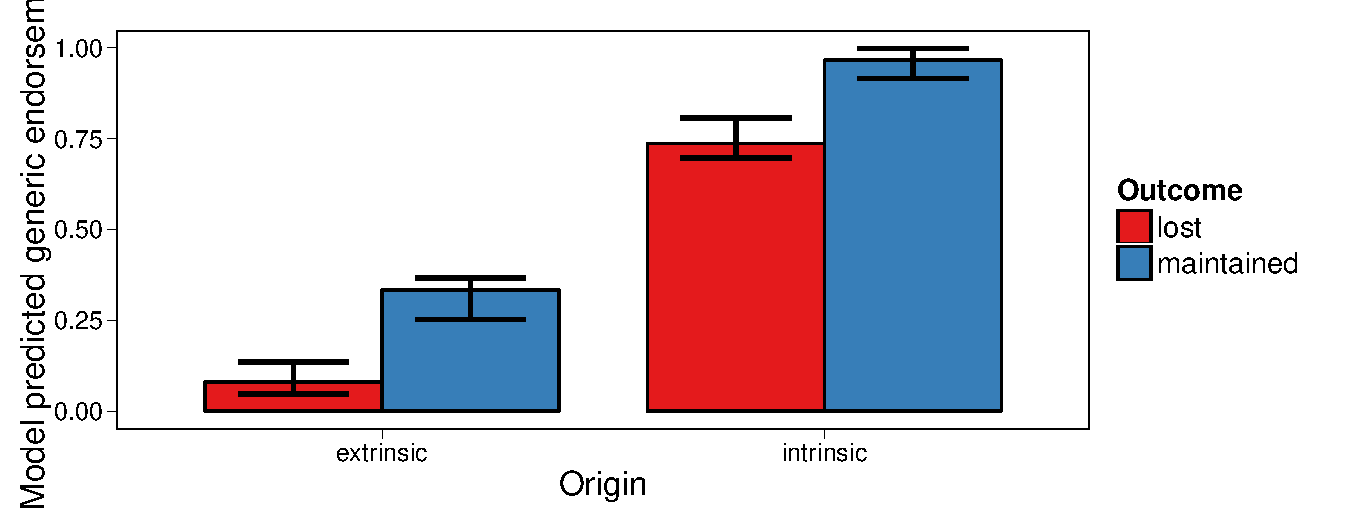
\includegraphics[width=0.5\columnwidth]{dobles-model.pdf} \\
    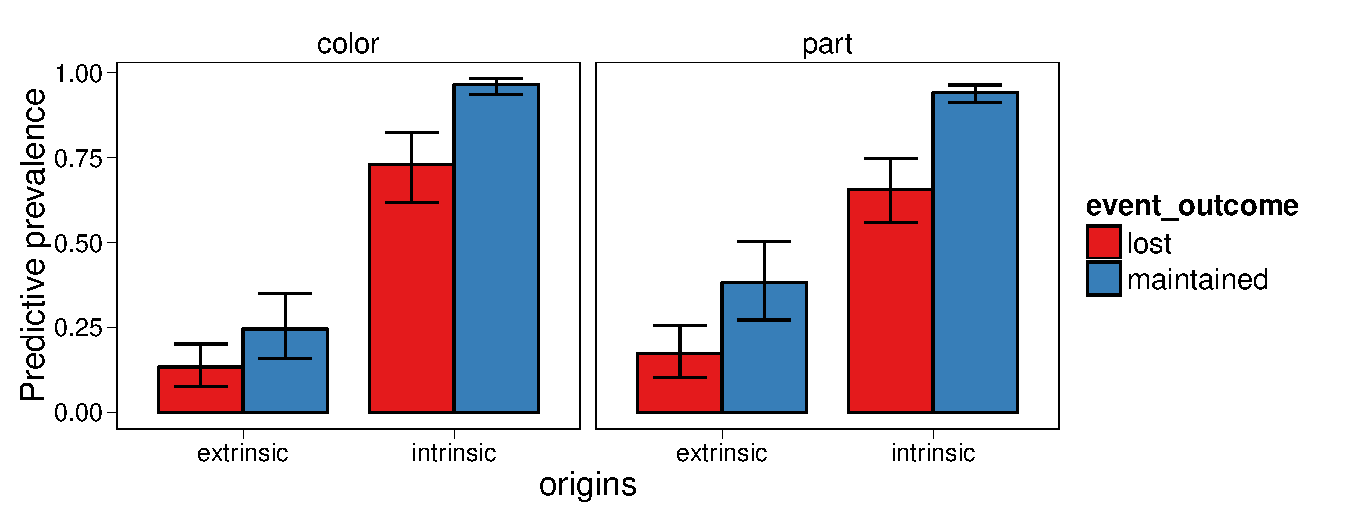
\includegraphics[width=0.5\columnwidth]{dobles-predictive-byItem.pdf} &
      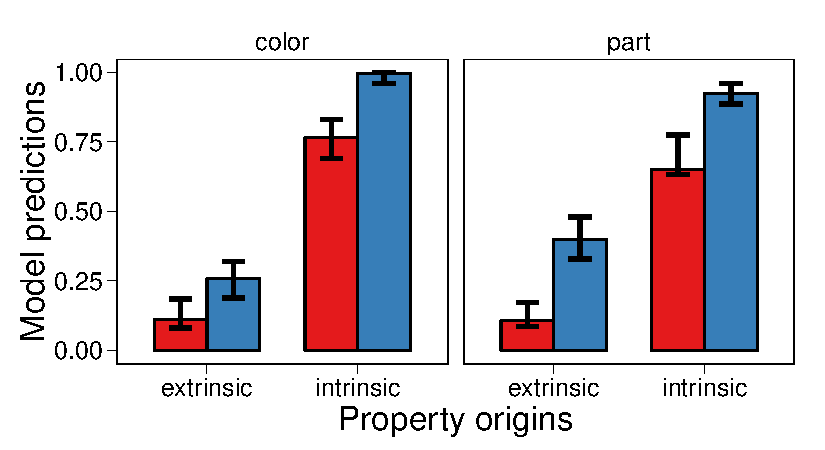
\includegraphics[width=0.5\columnwidth]{dobles-model-byItem.pdf} \\
\end{tabular}
    \caption{
    (a) Average predicted probability of a future creature having the property. (b) Truth judgment model predictions given the predicted prevalence in (a).
    Bottom row shows data and predictions broken down by item.
  }
  \label{fig:dobles-predictive}
\end{figure*}

\section*{Experiment 3b: Truth judgment task}

In this experiment, we test the predictions of our model using a truth judgment measure in the same paradigm.

\subsubsection*{Participants}
We recruited 80 participants over MTurk.  
The experiment took about 3 minutes and participants were compensated \$0.35.
None of the participants completed Experiment 3a as well.

\subsubsection*{Procedure and materials}
The procedure and materials are exactly the same as in Expt.~3a, with the exception of the dependent measure.
After reading each vignette, participants were asked: ``Do you agree or disagree that: \textsc{generic statement} (e.g. Dobles have claws)''.
Participants responded by choosing one of two radio buttons corresponding to agree or disagree.

\subsubsection*{Results and discussion}

%                                         Estimate Std. Error z value        Pr(>|z|)    
%(Intercept)                               -2.9444     0.5130  -5.740 0.0000000094624 ***
%event_outcomemaintained                    2.6931     0.5603   4.807 0.0000015342262 ***
%originsintrinsic                           3.6753     0.5658   6.496 0.0000000000824 ***
%event_outcomemaintained:originsintrinsic   0.2396     0.9400   0.255           0.799    

Our pragmatics model with the elicited predicted prevalence from Expt.~3a made two novel predictions for this experiment: (1) in addition to a main effect of origins, we would find a main effect of event outcome; (2) this effect would be stronger for body part properties than for color properties.
As predicted, we found two main effects (Figure \ref{fig:dobles-results}a).
The main effect of property origins replicated ($\beta=3.6, SE=0.57, z=6.5, p<1\text{e}10$): participants were more likely to endorse the generic when it was about a property that the creature was born with.
As well, we find a second main effect of event outcome 
 ($\beta = 2.69, SE = 0.56, z=4.8, p<1\text{e}5$): participants were more likely to endorse the generic when the property was maintained than when it was lost.
\footnote{
To see whether this second main effect could be attributed to a subgroup of participants making their judgments based only on the final screen (which showed creatures with or without the property, depending on  the event outcome), we classified each participant according to their pattern of responses. 
Just as many participants endorsed the generic based on the final screen alone (``Only outcome''; 19) as there were basing their endorsement on both the outcome and the origins (``Both outcome and origins'' ; 16).
36 participants based their responses on only the origins, and 9 participants exhibited some other pattern of responses.
Thus, it seems this effect is not due to a subgroup of participants basing their responses on only the final screen.
}

%\begin{table}[]
%\centering
%\begin{tabular}{@{}lllll@{}}
%\toprule
%  & Only origins & Only outcome & Both & Neither \\ \midrule
%n & 36           & 19           & 16   & 9       \\ \bottomrule
%\end{tabular}
%\caption{Numbers of participants ($N=80$) who made their generic endorsement based on different factors.}
%\label{tab:dobles}
%\end{table}


 
When we break down the results by item, we see that this effect is  stronger for body part properties than for color properties (Figure \ref{fig:dobles-results}b).
The endorsement of a generic for color properties (e.g. \emph{Lorches are green}) seems to be less sensitive to the outcome of the event (i.e. Lorches losing their color as a result of drinking a chemical).
This may be due to participants' intuitive theories of properties and their stability (skin color is more stable than body parts like feathers).
Indeed this difference is apparent in the predictive prevalence task (Expt.~3a).
For the 8 data points of generic endorsement based on origins, outcome, and property type, our model's predictions match the data well ($r^2(8) = 0.96$; see Figure \ref{fig:dobles-predictive}b, bottom).
We, thus, elaborate our theory.
The semantics of generics can be understood as a threshold on property prevalence, though prevalence is a speaker's subjective belief about what is likely to be the case in the future.

\begin{figure*}
\begin{tabular}{l l}
(a) & (b) \\
\\
\centering
    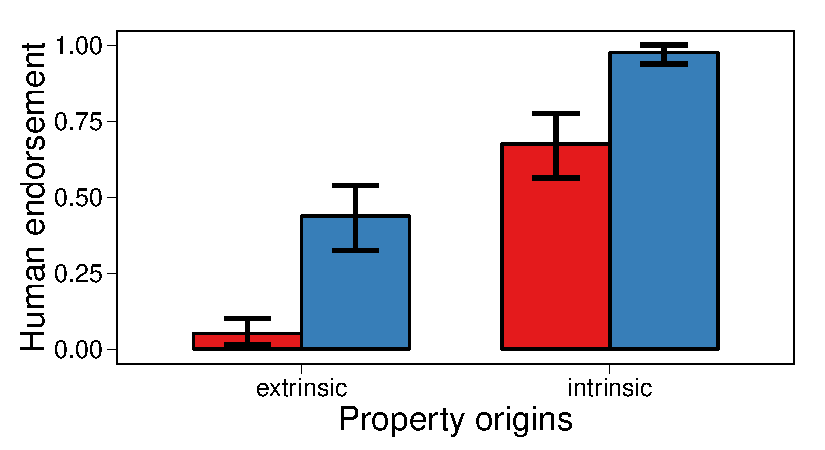
\includegraphics[width=0.5\columnwidth]{dobles-results.pdf} &
    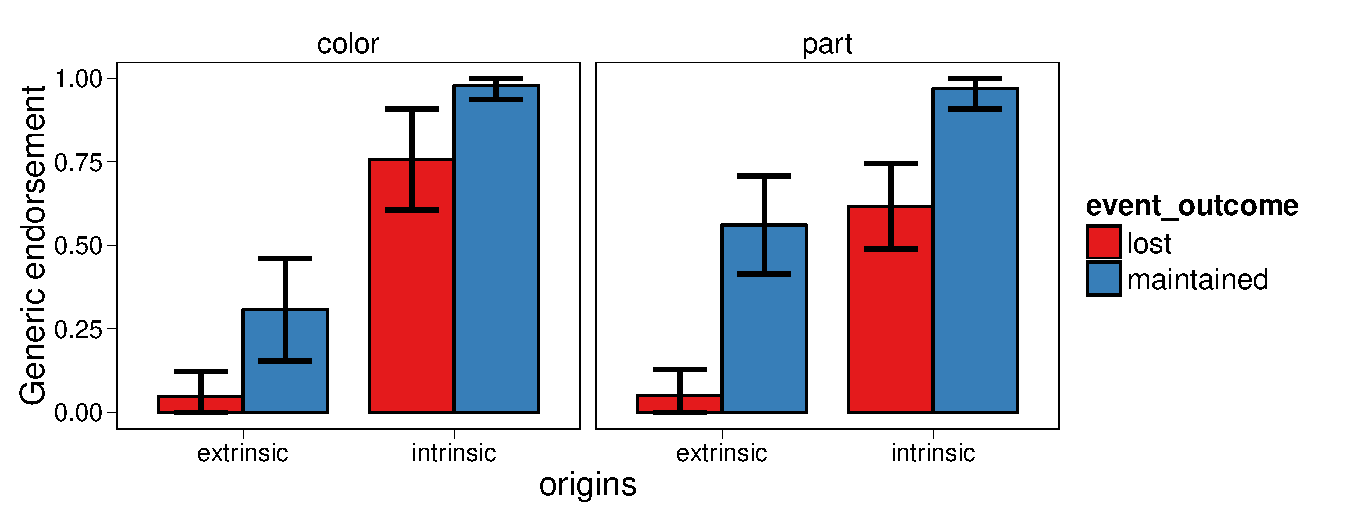
\includegraphics[width=0.5\columnwidth]{dobles-byItem-results.pdf} \\
\end{tabular}
    \caption{
    (a) Average endorsement of the generic statement in Expt.~3b (replication of Gelman and Bloom (2007)). (b)  Results broken down by type of item.
  }
  \label{fig:dobles-results}
\end{figure*}




\section*{General discussion}

Generic language expresses dramatic flexibility that has confounded psychologists, linguists and philosophers who have tried to articulate what makes generic statements true or false. 
We evaluated a theory of generic language derived from general principles of pragmatic language understanding using a simple, but uncertain, basic meaning---a threshold on property prevalence.
Our formal model is a minimal extension of the RSA theory of language understanding, together with an underspecified threshold semantics.
The model was able to explain two major puzzles of generics: their extreme flexibility in truth conditions and the contrastingly strong interpretation of novel generics.
Both of these phenomena were revealed to depend in systematic ways on prior knowledge about properties.
This prior knowledge was revealed through Bayesian model analysis to be structured, providing a promising bridge to conceptual accounts of generic language.
In the final experiment, we tested the novel prediction that generic language is about speakers' expectations of future prevalence, and not necessarily what the current world is like. 
Across all experiments, the formal model predicted the quantitative details of participants' judgments with high accuracy.

%generics have a simple but uncertain basic meaning---a threshold on property prevalence---which is refined by social reasoning.
%a minimal extension of a general-purpose probabilistic model of language understanding wherein social-cognitive mechanisms act on uncertainty in the meaning of a generic utterance to produce a less uncertain meaning.
%Model predictions for interpretation of generic sentences depend on the listener's beliefs about the property in question and the communicative force of a speech-act. 
%The model predicted participants' judgements with high quantitative accuracy for both goodness judgements for natural generic sentences, and interpretation of novel generic sentences.
%Our model both the role of the speaker to produce felicitous generic utterances and the role of the listener to interpret those utterances in context, with high quantitative accuracy.
%general-purpose language understanding mechanisms are 



%%this paragraph isn't needed and is confusing....
%Interpretation of generic language is strongly governed by listeners' beliefs about the domain in question. 
%The generic, it would seem, doesn't convey any additional information beyond what the liste	ner already knew about the domain.
%This shouldn't surprise us. 
%In much the same way, ``John is tall'' does not actually tell a listener about what \emph{tall} means\footnote{However, ``John is a person'' does tell a listener about what \emph{tall} means in ``John is tall''.}. 
%Rather, the listener is expected to come to the conversation with some beliefs about heights, and knowing that John is a person, be able to infer likely meanings for \emph{tall}.

\subsection*{Evidence against prevalence-based accounts}

%The truth conditions of generic language have been of interest to linguists and philosophers. 
There have been numerous demonstrations arguing that prevalence is insufficient to explain generic meaning \cite{Gelman2002, Gelman2007, Cimpian2010, Cimpian2010c,Khemlani2012, Prasada2013}.
We agree with the spirit of these claims, but disavow the conclusions.
Prevalence is usually framed as a ``null hypothesis'', bordering on straw-man.
It is usually instantiated by measuring only the prevalence of the property for the target category \cite<e.g. the percentage of birds that lay eggs; >{Khemlani2012, Prasada2013}.
It is what we have referred to as within-kind prevalence and it also fails to explain our data (Figure \ref{fig:commongenerics}b, right).

Some have identified \emph{cue validity} to be a statistical factor in generic truth conditions \cite<e.g., >{Khemlani2012}.
Cue validity is defined as the probability of the kind given the feature: $P(K \mid F)$ (e.g. the probability that an animal is a mosquito given that it has malaria).
%By Bayes' rule, cue validity must take into account the prevalence of the property in the kind and the prior probability of that kind $P(K \mid F) \propto P(F \mid K) \cdot P(K)$. 
It should be noted that our mixture parameter $\phi$ (the potential of the property to be present in a kind) is a different statistic from cue validity.
Cue validity is defined with respect to a particular kind and property, whereas our mixture parameter is only defined with respect to a property.
In some cases, the two can be similar.
For instance, \emph{having a mane} is a good cue for being a \emph{lion} and similarly \emph{has manes} has a low $\phi$ parameter (since it is not present in many kinds). 
In other cases, it is clear that the two constructs are distinct.
For the property \emph{eats people}, the mixture parameter $\phi$ is again very low because most animals don't eat people; yet learning that some animal \emph{ate a person} is not a particularly good cue for any one kind of animal.
Additionally, unlike a data-analytic model (e.g., a regression model) that uses predictors of prevalence and cue-validity to \emph{describe} data, our model is a unified cognitive model --- a formal instantiation of an explicit psychological hypothesis --- that \emph{predicts} both generic endorsements and interpretations from a simple set of assumptions (a prior belief distribution and general pragmatic computation).

\subsection*{The nature of the contrast class and individual differences}

In this paper, when accurately taking into account the shared knowledge that forms interlocutors' prior belief distribution, the puzzles of generic language are amenable to the basic principles of communication.
The prior belief distribution for a property (e.g., lays eggs), is a distribution over kinds (and their associated prevalence of the property).
We might refer to these other kinds as the \emph{contrast class}.
This is analogous to how if we say of 10 year-old Abigail that ``Abigail is tall'', we mean she is tall relative to the contrast class of other 10 year olds, or perhaps 10 year old girls.

Like almost all of the extant psychological work on generics, we have focused our efforts on simple sentences about natural kinds, particularly animals.
In addition to being the main focus of past theoretical and empirical work, focusing on animals is methodologically convenient as the contrast class for animal properties is quite plausibly \emph{other animals}.
Indeed, this assumption was explicit in our first experiment, where we elicited  property prevalence for many different animal kinds. 
As we move away from statements about animals, or even natural kinds, determining what goes into the contrast class becomes a lot more complicated. 

There are some hints that the contrast class can be derived with respect to the property \cite{Keil1979}.
For example, the statement ``iPhones are useful'' could be in contrast to other forms of technology (like a desktop computer), while ``iPhones are heavy'' could really only be true relative to other handheld devices.
This could be another way for the slipperiness of generics to manifest; if a speaker and listener fail to coordinate on the same contrast class, our theory predicts disagreements as to the veracity of generic claims.

Other failures to coordinate could result in individual differences in generic endorsements as well.
In addition to differences in the contrast class, our theory proposes individual differences may result from disagreements in the target-kind prevalence as well as in the distribution of prevalence.
For example, there is considerable disagreement as to whether or not ``Humans cause global warming''.
Our theory predicts this disagreement may be the result of differences in the estimated \emph{causal power} of humans influencing global warming as well as the causal power of \emph{other forces} (e.g., plate tectonics) on climate change.
This is a promising area for future research.

\subsection*{The parallel problem of generic identification}

Throughout this paper we treated the bare plural construction as a generic utterance with a threshold semantics: $\denote{\text{K F}}(x, \theta)=x>\theta$.
The bare plural construction can also indicate a specific plural predication.
For example, ``Dogs are on my lawn'' picks out a specific group of dogs, while ``Dogs have fur''  does not \cite{Carlson1977}.
The problem of \emph{identifying} a generic meaning from a bare plural construction is itself a hard problem because generic meaning can be signaled using a diverse array of morphosyntactic cues.

\citeA{Declerck1991} suggests that generic and non-generic bare plurals can be treated in the same way, and that pragmatic considerations alone may resolve interpretative differences. 
Indeed it does appear that knowledge of the properties under discussion (e.g., the state of being on a front lawn; the state of having fur) could facilitate the generic identification process.
Other pragmatic factors, like knowledge of the speaker, can also disambiguate generic and non-generic meaning \cite{Cimpian2008}.
The formal theory introduced in this article couches generic language understanding in a communicative framework.
Addressing the question of generic identification from an information-theoretic, communicative perspective is a natural extension.

%There is some promising evidence to suggest this process may be pragmatic as well , Declerck1991}. 
%For instance, 
%We find this idea plausible.
%Consider, for example, the probability of animals being on your front lawn. 
%It is extremely unlikely for there to be many instances of \emph{any} animal on your front lawn (due to the spatial constraints of your lawn, and the lack of any good reason for an animal to be on your lawn). 
%Thus, the prior distribution over the probability would likely resemble that of an accidental property (Expt.~2a).
%Future work should address the relation between the prevalence priors and actual numbers of instances that can be observed.
%The $L_1$ listener model would in this case, interpret that bare plural as implying that just a few instances of dogs were on your front lawn. 

%In this paper, we concerned ourself with the problem of generic meaning, once a generic utterance has been identified as such. 
% the interpretation of a truly generic utterance, once identified as such.

%The puzzle of generic \emph{meaning} is often contrasted with the problem of generic \emph{identification}. 
%Within this line of thinking, a sentence is hard to identify as conveying a generic meaning because generic meaning can be signaled using a number of morphosyntactic forms. 
%For example, both \emph{Dogs are friendly} and \emph{A dog is friendly} are thought to both signal a generic interpretation.
%Additionally, the morphosyntax alone is not a sufficient cue to generic meaning: \emph{Dogs are friendly} conveys a generic meaning while \emph{Dogs are on my front lawn} does not.




%We should note that we did not directly measure $P(K \mid F)$ in our studies, though it can derived from our prevalence distributions using Bayes' rule
%$$
%P(K \mid F) \propto P(F \mid K) \cdot P(K)
%$$
%Specifying what functional form $P(K)$ should be is not obvious: For instance, is $P(K)$ a uniform distribution over all possible animal kinds, or is it subject to how typical an animal each kind is?

%\mht{Probably will add a discussion of empirical claims against prevalence, and how prevalence in our theory is about \emph{subjective probability} which is tied to both people's abstract beliefs and to the state of the world.}



\subsection*{Implications for conceptual structure}


Previous psychological and philosophical work on generics has looked beyond prevalence and focused on conceptual distinctions and relations \cite{Gelman2003,Prasada2013,Leslie2007,Leslie2008}. 
\citeauthor{Prasada2013} has argued for a distinction between \emph{characteristic} properties (e.g.~\emph{Diapers are absorbent.}) and \emph{statistical} properties (e.g.~\emph{Diapers are white.}).
Leslie suggests information that is striking (e.g.~\emph{Tigers eat people.}) is useful and thus permitted to be a generic.
Gelman outlines how generics tend to express \emph{essential} qualities that are relatively timeless and enduring. 
Where in the prevalence-based semantics could such conceptual distinctions come into play?

Our theory claims that causal beliefs about kinds and properties lead to differences in prevalence distributions, and these differences lead to variable endorsements and interpretations of generic sentences for our formal model. 
In Expt.~2, we showed how the structure of prevalence priors about different kinds of properties leads to variable inferences. 
Biological properties tend to have bimodal prior distributions on prevalence (with 0\% and 100\% prevalence being the most likely \emph{a priori}) and get updated, upon hearing a generic, to concave posterior distributions peaked at 100\%.
Accidental properties have unimodal prior distributions (peaked at only 0\%). 
This distinction arises because even when participants learn the property is present in one instance of the category, they were unwilling to extend it to many others of the category \cite{Goodman1955}. 
In this case, this prior distribution of prevalence for accidental properties gets updated to a convex posterior distribution.
This posterior distribution has high variance, indicating that interpretations of generic statements about accidental properties should be highly variable.
These predictions were corroborated by the empirical data of Expt.~2b. 

Thus, our approach makes the strong claim that beliefs about predicted prevalence are the connective tissue between conceptual knowledge and generic language.
That is, the effect of conceptually meaningful differences on generic language is predicted to be mediated by differences in corresponding prevalence distributions.
And though prevalence may not be consciously by the interlocutor when thinking about generics, the theory presented here suggests that this statistical information is along for the ride. 
Indeed, we found that empirical prevalence distributions are structured in a way that reflects intuitions about causal mechanisms underlying different properties.
It is plausible that richer conceptual knowledge also influences these distributions, such as higher-order conceptual knowledge about the nature of properties and categories \cite{Gelman2003,Keil1992}. 

It has been argued that conceptual structure takes the form represented by probabilisitic causal models \cite{pearl1988probabilistic, Gopnik2003theory, Goodmanconcepts}. 
Such a representation would give rise to the prevalence distributions we observed are so crucial for understanding generic language. 
Further work will be needed to make connection from the prevalence distributions uncovered here to probabilisitic causal models.

Finally, it is important to note that our approach is based on \emph{subjective} probability, and not mere frequency.
Indeed, we elucidated in Expt.~3, that participants' \emph{predictions} of probability perfectly track generic endorsement, when the present frequency would not hold.
This resolves another theoretical issue in the generics literature: Current frequency is not sufficient.%\footnote{This is usually paired alongside ``Frequency is not necessary'' and given the example of ``Mosquitos carry  malaria''.}
The classic example of this phenomenon is the statement ``Supreme Court Justices have even social security numbers'', which is predicted by linguists to be rejected even if every single Supreme Court Justice has an even social security number.
Our explanation is that abstract intuitive theories lead us to reject observed frequencies in forming our subjective probabilities.
That is, because we may believe selection for the Supreme Court is not influenced by one's social security number, we would assign roughly 50\% subjective probability to the \emph{next} justice having an even number.
Thus, we would still reject the generic \emph{Supreme Court Justices have even social security numbers}, because the predictive prevalence would not be any different for Supreme Court Justices than any other profession. 
Our perspective makes the intriguing prediction that if we learned much more surprising information, such as all justices having \emph{prime numbered} social security numbers (a probabilistically much less likely outcome to happen by random sampling), we might be compelled to revise our theory, for instance appealing to a conspiracy; perhaps in this case, we might accept the generic.
The relationship between conceptual distinctions, subjective probabilities for prevalence, and generic language is another area of research opened up by this work. 

%We do not disagree with these claims. 
%Rather than carve out the distinctions amongst generics, we highlight what is shared. 

%, and that generic language can increase the psychological coherence of a category.
%\citeA{GelmanEtAl2004} finds that child-parent conversations contain many more generics about animal kinds than about artifact kinds, possibly owing to the belief that animal kinds are more richly structured than artifact kinds. 


%Finally, there are compelling demonstrations that causal beliefs about properties are the driving force behind the various interpretations of generic statements \cite{Gelman2007, Cimpian2010c}.
%\citeA{Gelman2002} demonstrated that children and adults believe the prevalence implied by a novel generic utterance (e.g. \emph{Bears like to eat ants.}) is high, but distinct from quantifier statements like ``some'' or ``all''. 
%The properties used in this experiment were plausible construed as biological or essential \cite{Gelman2003}.
%This work was conceptually replicated by \citeA{Cimpian2010} with novel categories (e.g. \textsc{lorches}) and extended to show that the strong interpretation of generics could be weakened by predicating the kind with accidental properties (e.g. \emph{Lorches have muddy feathers.}).
%

%This falls out of basic principles of communication. 
%Information is can only be informative with respect to some prior beliefs.
%
%
%Generic language has been of interest to psychologists primarily because of its ubiquity in natural conversation and its role conceptual development.







%\mht{say something about development?}


%Beliefs about prevalence in our approach are represented as probability distributions, a framework that is useful for representing rich, structured knowledge of the world \cite{Goodmanconcepts}. 




%
%For example, communicating subjective probability should be useful for future prediction and so if speakers hold the higher-order belief that some observations or states are transient and not predictive of future events (e.g. all U.S. Supreme Court Justices having at this moment social security numbers that are all prime numbers), their estimates of the subjective probability to communicate will be less influenced by this state; this will cause speakers to hesitate to assert the corresponding generic (\emph{Supreme Court Justices have prime numbered social security numbers}).


%To highlight one example, individuals may believe some observations are the result of accidents and are not predictive of future instances (e.g. all of the Supreme Court Justices having even-numbered social security numbers). 
%The corresponding generic (i.e. \emph{Supreme Court Justices have even-numbered social security numbers.}) may lack support because the corresponding conceptual models do not have any strong causal mechanism that could have given rise to the observation, and thus the prevalence of the property in the future (i.e. the predictive prevalence) will not be similar to the present prevalence. 
%In our experiments, we have focused on properties that are plausibly construed of as essential (e.g. \emph{lays eggs}, \emph{has feathers}) and thus predictive of future instances. 
%We found that a set of plausibly temporary properties (e.g. \emph{has muddy feathers}) are interpreted as implying a much lower percentage of the kind with the property than the biological properties, suggestive that the accidental nature of the property influences interpretations of prevalence.


%The results of these studies, as well  future research and model development.

%How interlocutors arrive at estimates of the prevalence, and what other inferences are licensed in a context, may be the result of a deeper conceptual model of the world. 

\subsection*{Conclusion}

It might seem paradoxical that a part of language that is so common in communication and central to learning should be vague. 
Shouldn't speakers and teachers want to express their ideas as crisply as possible?
To the contrary, underspecification can be efficient, given that context can be used to resolve the uncertainty \cite{Piantadosi2012}.
In our work, context takes the form of a listener and speaker's shared beliefs about the property in question. 
By leveraging this common ground, generics provide a powerful way to communicate and learn generalizations about categories, 
which would otherwise be difficult or costly information to learn through direct experience.
%This, coupled with standard inferences from conversational pragmatics, allows the listener to arrive at a specific meaning of the otherwise underspecified utterance.
The dark side of this flexibility is the potential for miscommunication or deceit: A speaker might assert a generic utterance that he himself would not accept, conveying a too-strong generalization to a na\"{i}ve listener.  
Our model predicts this potential particularly for properties which, when present, are widespread in a category---we showed that biological properties are believed to have this distribution, but many properties of social categories may as well \cite{Cimpian2011a,Cimpian2012b,Rhodes2012}.
%This listener would then have a belief distribution even further from the truth. 


Categories are inherently unobservable. 
You cannot see the category \textsc{dog}, only some number of instances of it.
Yet we easily talk about these abstractions, conveying hard-won generalizations to each other and down through generations.
The theory presented here gives one explanation of how we do so, providing a computational perspective on how category generalizations are conveyed and how beliefs play a central role in understanding language.






%\section*{Materials}
%%\begin{materials}
%%Details are given in the {\it SI Materials and Methods}.
%\subsection{Generics model}
%The generics model was implemented using the probabilisitic programming language WebPPL \cite{dippl}. 
%The model, once $P(x)$ is fixed, has one free parameter: the speaker rationality parameter $\lambda$ in Eq.~\ref{eq:S1}. 
%Because $\lambda$ is not of theoretical interest here, it is marginalized in accord with Bayesian data analysis principles \cite{LW2014}.
%Both the prevalence  x$\in$[0, 1]  and the threshold  $\theta \in$[0, 1] were discretized to permit exact enumeration of the posterior.
%The prevalence scale was discretized into 11 bins --- \{0, 0.01, 0.1, 0.2, ... , 0.8, 0.9, 0.99\} --- and the threshold scale into 10 bins ---  \{0, 0.1, 0.2, ... , 0.8, 0.9\}. 
%The results are the same when a 21, 20 bin discretization is used. 
%A fully specified version of the generics model, as well as the structured prior model (described below), can be found at http://forestdb.org/models/generics.html. 









%\appendix[Structured, Bayesian model of the prior elicitation task]


%\end{materials}
%
%\begin{acknowledgments}

\subsubsection*{Author contributions}
M. H. Tessler and N. D. Goodman developed theory and the study concept and design.
M. H. Tessler performed research and analyzed data.
M. H. Tessler and N. D. Goodman wrote the paper.

\subsubsection*{Acknowledgements}

This work was supported in part by National Science Foundation Graduate Research Fellowship DGE-114747 (to M.H.T.),
by John S. McDonnell Foundation Scholar Award 220020252 (to N.D.G.) and 
Office of Naval Research Grant N00014-13-1-0788 (to N.D.G.)

\newpage
\bibliographystyle{apacite}

\setlength{\bibleftmargin}{.125in}
\setlength{\bibindent}{-\bibleftmargin}

\bibliography{generics}

\newpage


\section*{Appendix A: The Rational Speech-Acts framework}

The goal of this section is introduce the reader to the Rational Speech-Acts framework and point to various applications and areas of ongoing research when relevant.

The Rational Speech-Acts theory views language understanding as a special case of social cognition instantiated in a Bayesian model \cite{Frank2012, Goodman2013}. 
In this view, an utterance is \emph{interpreted} by a Bayesian listener by integrating her prior beliefs with her generative model of the utterance.
The generative model of the utterance is her intuitive theory of speech \emph{production}, i.e. her theory of a speaker. 
This intuitive theory of speech production views speakers are rational actors who behave in accord with Bayesian decision-theory \cite{berger1988}.
The rational speaker, thus, chooses utterances soft-max optimally on the basis of certain goals.
In RSA, the goal of is to convey information to a naive listener. 
The pragmatic listener ``inverts'' her Bayesian model of a speaker to arrive at a pragmatic interpretation of an utterance.

This model is posed at the computational or rational level \cite{Marr1980, Anderson1991}. 
It is not intended as an explicit model of the \emph{process} of language comprehension; rather, it is a computational model of pragmatic competence under the cooperative principle \cite{Grice1975}. 

In simplest form, a pragmatic listener ($L$) is interested in learning about the world $x$ upon hearing an utterance $u$. 
$$
P_{L}(x  \mid u) \propto P_{S}(u \mid x) \cdot P(x) \label{eq:RSA_L}
$$
She does this by integrating her prior beliefs about the world $P(x)$ with the likelihood that a speaker ($S$) would have produced the utterance $u$ given a world $x$: $P_{S}(u \mid x)$.
Prior beliefs about the world $P(x)$ capture relevant world-knowledge, which is central to deriving context-specific interpretations \cite{Degen2015cogsci}.
The production model $P_{S}$ is defined recursively with the listener model: The speaker produces an utterance according to a utility function, which is a soft-max function of the probability that the listener would infer the world $x$ given the utterance $u$: $P_{L}(x  \mid u)$, jointly with the prior probability of the utterance $P(u)$.
$$
P_{S}(u \mid x) \propto \exp{(\lambda \cdot \ln (P_{L-1}(x  \mid u) ) )} \cdot P(u) \label{eq:RSA_S}
$$
$\lambda$ it the ``speaker optimality'' parameter: It governs the degree to which the speaker values informativity when producing an utterance. The speaker is not perfectly Bayesian because he is assumed to be a rational actor (not just a belief-updater), and takes actions soft-max optimally in accord with his posterior belief distribution \cite{Baker2009}.

The prior probability of an utterance $P(u)$ can include information about an utterance's cost or complexity as well as the alternative utterances available to a speaker. 
Manipulating an utterance's cost has been used to derive Manner implicatures \cite{Bergen2016}, though in many applications utterance cost is kept uniform across alternative utterances. 
The specification of alternatives is an area of ongoing research \cite{Franke2014cogsci, Peloquin2016} and is currently determined by the modeler for the problem at hand.

The recursive speaker--listener model requires a base case in order to make predictions. 
RSA adopts the notion from formal semantics that there is a literal meaning, or a context-invariant mapping, from utterances and worlds to truth values:  $\denote{u}: X \rightarrow \text{Boolean}$. 
From this, we construct a base case of a \emph{literal listener}, who interprets utterances with respect to their literal meaning.
%
$$
P_{L_{literal}}(x \mid u ) \propto {\delta_{\denote{u}(x)} \cdot P(x)} \label{eq:RSA_L0}
$$
Note that this model is the same as $P_L$ except for the likelihood function. 
%
Here, the likelihood $\delta_{\denote{u}(x)}$ is the Kronecker delta function returning $1$ for states $x$ compatible with utterance $u$, and $0$ otherwise.

The Rational Speech-Acts model formalizes the Gricean maxim to be information: The speaker produces utterances not with respect to their literal meaning, but with respect to how a naive listener (the literal listener) would interpret them, given the literal meaning and the listener's prior beliefs\footnote{Technically, this is what the listener believes the speaker believes is her prior beliefs.}.
This literal listener base case also gives us the Gricean maxim to be truthful: the speaker who reasons about the literal listener has the goal of communicating the state $x$ given an utterance $u$ and given its literal meaning $\denote{u}$. 
In principle, the speaker--listener recursion could grow for ever. 
In practice, stable pragmatic phenomena can be observed with just one level of recursion. %\red{(CITE something?)}. 

%\mht{This paragraph is pretty abstract, and may be better suited for the discussion}
This general framework has been applied to host of language and reasoning phenomena including understanding scalar implicature \cite{Goodman2013, Degen2015cogsci}, communication in a noisy channel \cite{Bergen2015}, question--answer behavior \cite{Hawkins2015}, syllogistic reasoning \cite{Tessler2014}, and figurative language including hyperbole \cite{Kao2014}, metaphor \cite{Kao2014b}, and irony \cite{Kao2015}.
In addition, RSA has been used to bridge the semantics--pragmatics divide, by using pragmatic reasoning to understand the very meaning of words in domains where literal meanings are hard to specify \cite<e.g. vague adjectives such as \emph{tall}, >{Lassiter2015}.
These applications often extend RSA by introducing an additional random variable for the pragmatic listener. 
For example, in addition to the listener being uncertain about the state of the world ($x$, above), she may have uncertainty about what is in common ground, what is the topic being discussed, and even what is the very meaning of the word. 
These kinds of uncertainty can plausibly be posited both at the pragmatic level ($L$) and/or at the base-case, the literal listener. 
However, empirical studies show that the richness of human pragmatic inference depends on this uncertainty being available at the pragmatic level. 
This is because uncertainty at the pragmatic level can be resolved incorporating the Gricean pressure to be informative, which only manifests at levels of recursion beyond the base case.
%We now return to the question of what a pragmatic theory of generic meaning would look like.

%The fact that pragmatic reasoning can be used for semantic inference (i.e. for learning the meaning of words) is suggestive that the difference between semantics and pragmatics is at least a little bit fuzzy.

%\begin{itemize}
%\item Scalar implicature example
%	\begin{itemize}
%		\item Language understanding as social cognition
%		\item Listener believes speaker is informed (speaker conditions on observed state)
%		\item Listener believes speaker is helpful (speaker has model of a naive listener)
%	\end{itemize}
%\item Computational level theory
%	\begin{itemize}
%		\item Does not say that this is explicit reasoning
%		\item Does not make developmental predictions
%	\end{itemize}
%\item Pragmatics and semantics vis a vis \emph{tall}
%	\begin{itemize}
%		\item Distinction gets blurred with adjectives, whose meaning gets computed certainly without regard to explicit reasoning
%	\end{itemize}
%\end{itemize}

\newpage
\section*{Appendix B: Model parameter posteriors}


\begin{figure*}[h]
\centering
    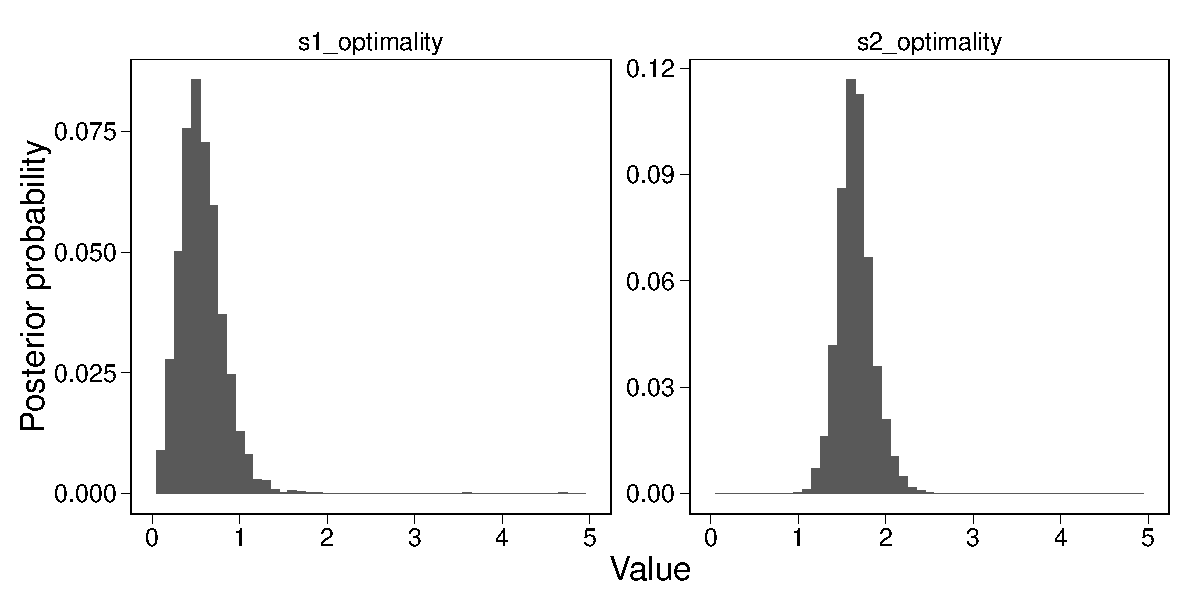
\includegraphics[width=\columnwidth]
    {familiar-truthjudgments-parameters.pdf}
    \caption{
    Posterior distributions for truth judgments model parameters (Expt.~1b)
}
  \label{fig:tj1-params}
\end{figure*}


\begin{figure*}[h]
\centering
    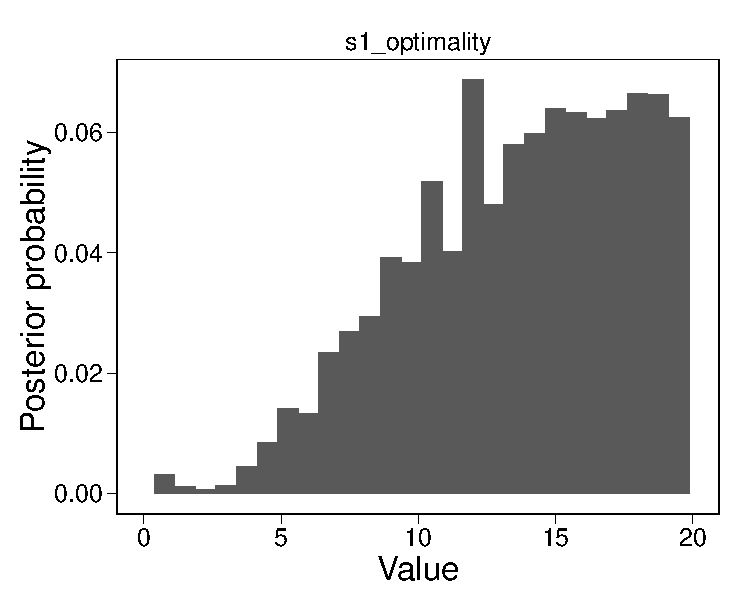
\includegraphics[width=0.6\columnwidth]
    {unfamiliar-interpretations-parameter.pdf}
    \caption{
    Posterior distributions for model parameter (Expt.~2b)
}
  \label{fig:interpretation-param}
\end{figure*}

\begin{figure*}[h]
\centering
    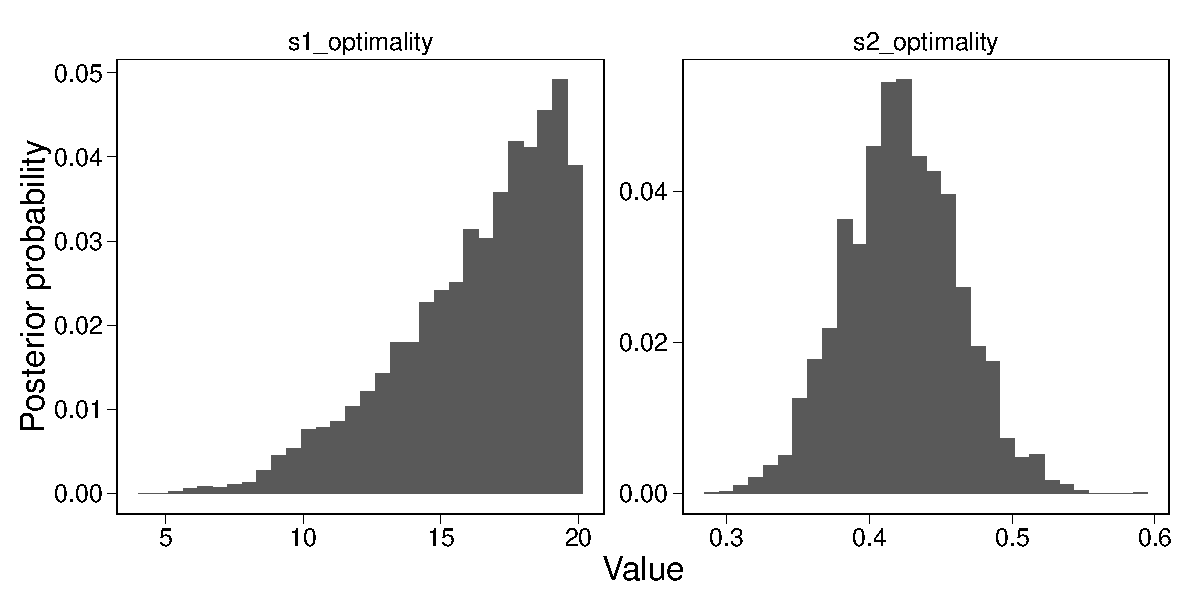
\includegraphics[width=\columnwidth]
    {unfamiliar-asymmetry-parameters.pdf}
    \caption{
    Posterior distributions for model parameters (Expt.~2c)
}
  \label{fig:asymmetry-params}
\end{figure*}

\begin{figure*}[h]
\centering
    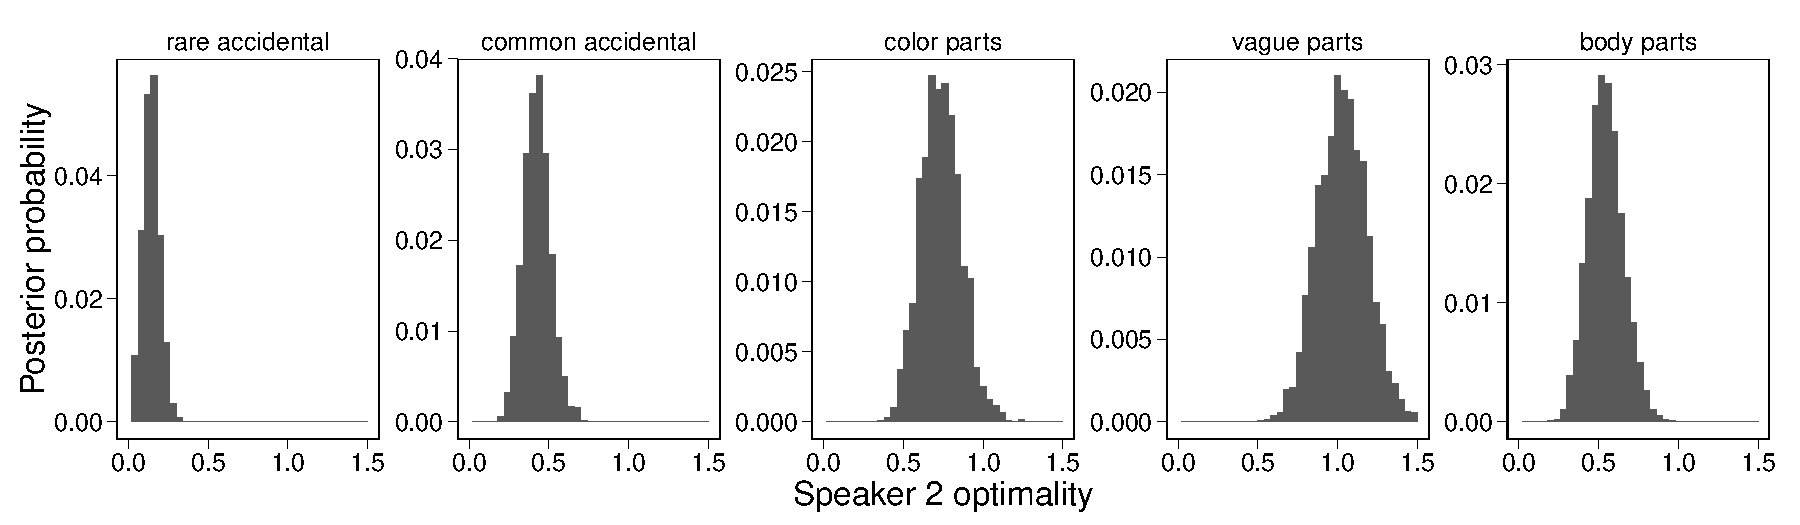
\includegraphics[width=\columnwidth]
    {unfamiliar-asymmetry-byItem-parameters.pdf}
    \caption{
    Posterior distributions for $\lambda_2$ inferred independently for each item type (Expt.~2c)
}
  \label{fig:asymmetry-params-byItem}
\end{figure*}

\newpage

\section*{Appendix C: Tables}




\begin{table}[h]
\centering

\caption{Stimuli used in Experiment 1. 
Estimates are proportion agreement for truth judgments and Maximum A-Posteriori (MAP) estimates for prevalence. 
Brackets denote 95\% confidence intervals for truth judgments and 95\% credible intervals for prevalences.}
\begin{tabular}{| l | l | p{3.5cm} | p{3.5cm} |}
\hline
Conceptual type & Item & Truth judgment & Prevalence \\
\hline \hline
Majority characteristic       & 1. Leopards have spots.    &0.956	[0.912, 0.989] & 92.7 [85.9, 99.0]\\
                                          & 2. Ducks have wings.                       &0.945	[0.89, 0.989] & 98.5 [95.2, 99.9]\\
                                          & 3. Cardinals are red.                       &0.989	[0.967, 1] & 75.5 [62.1, 86.9]\\
                                          & 4. Swans are white.                       &0.901	[0.835, 0.967] & 67.3 [57.1, 73.8] \\
                                          & 5. Peacocks have beautiful feathers. &  0.989	[0.967, 1] & 92.0 [77.7, 100] \\
Minority characteristic       & 6. Lions have manes.       &0.945	[0.89, 0.989] & 54.3 [48.1, 63.0]\\
                                          & 7. Kangaroos have pouches.                        &0.967 [0.923, 1]& 69.9 [65.8, 79.6]\\
                                          & 8. Robins lay eggs.                        &0.934	[0.879, 0.978]& 68.5 [61.1, 74.9]\\
Striking                      & 9. Sharks attack swimmers. &0.879	[0.813. 0.945] & 41.8 [32.0, 54.7]\\
                                  & 10. Mosquitos carry malaria.                        &0.989	[0.967, 1] & 47.2 [38.1,	 52.9]\\
                                  & 11. Ticks carry Lyme disease.                        &0.967	[0.923, 1] &  42.6 [40.0, 54.2]\\
                                  & 12. Tigers eat people.                        &0.692	[0.593, 0.78] & 37.3 [23.3, 49.9]\\
False generalization & 13. Robins are female.      &0.429	[0.33, 0.527] & 51.9 [47.8. 55.4]\\
                                              & 14.  Lions are male.                       &0.571	[0.473, 0.67] & 49.9 [46.6, 53.9]\\
                                         & 15. Swans are full-grown. & 0.725	[0.637, 0.802] & 59.7[51.0, 66.0]\\
                                         & 16. Leopards are juvenile. & 0.143	[0.077,0.22] & 28.3 [22.9, 38.2] \\
                                         & 17. Sharks are white. & 0.341	[0.253, 0.44] & 32.2 [15.8, 44.6] \\
False or Uncertain & 18. Leopards have wings.       &0.022	[0, 0.055]& 1.0 [0.0, 4.1]\\
                                              & 19. Kangaroos have spots.                       & 0.033 [0, 0.077]& 5.0 [0.1, 13.5]\\
                                              & 20.  Tigers have pouches.                       &0.011	[0, 0.033]& 2.0 [0.0, 12.3]\\
                                              & 21.  Robins carry malaria.                       &0.055	[0.011, 0.099]& 5.4 [1.6, 9.1]\\
                                              & 22. Sharks have manes.                       &0.044	[0.011, 0.099]& 0.3 [0.0, 5.7]\\
                                              & 23. Lions lay eggs.                       &0 [0, 0] & 0.1 [0.0, 4.3]\\
                                              & 24. Sharks don't attack swimmers.                       &0.231 [0.154, 0.319] & 59.3 [49.8, 75.1]\\
                                              & 25. Ticks don't carry Lyme disease.                       &0.044 [0.011, 0.088] & 55.1 [46.6, 60.8]]\\
                                              & 26. Mosquitos don't carry malaria.                       &0.077 [0.033, 0.132] & 58.7 [50.5, 65.3]]\\                                              
                                              & 27. Tigers don't eat people.                       &0.297 [0.198, 0.385]& 65.3 [56.9, 97.7]\\                                              
                                              & 28. Peacocks don't have beautiful feathers.                       &0.022 [0, 0.055] & 17.4 [0.5, 27.5]\\                                              
                                               & 29. Mosquitos attack swimmers.       &0.385 [0.286, 0.495] & 26.5 [8.4, 39.2]\\
			                         & 30. Sharks lay eggs.       &0.088 [0.033, 0.143] & 18.5 [0.6, 41.3]\\
\hline

\end{tabular}

\label{tab:expt1}
\end{table}

%\csvautotabular{novelKinds-prevalencePrior-byItem-gammaCIs.csv}

%\begin{table}[h]
%\begin{tabular}{| l || l | l | l |}
%   \bfseries Person & \bfseries Matr.~No.% specify table head
%    \csvreader[head to column names]{novelKinds-prevalencePrior-byItem-gammaCIs.csv}{}% use head of csv as column names
%    {\\\hline\Parameter	& \distinctiveness}% specify your coloumns here
%    \end {tabular}
%    \end{table}
    
\begin{table}[h]
\centering
\caption{Stimuli used in Experiment 2 and statistics of the priors measure in the prior elicitation task. 
\emph{Potential to be present} is a measure of how many different kinds are expected to have the property. Mean prevalence when present is a measure of how widespread the property is expected to be, assuming that it is present within a kind.
Maximum A-Posteriori (MAP) estimates and 95\% Highest Probability Density Intervals from the Bayesian data analysis model described in Section \ref{sec:bda2} are shown for each measure.
The majority of these items are taken from Cimpian et al. (2010)}
\label{tab:novelGenericsStimuli}
\begin{tabular}{| l || l | l | l |}
\hline
Property type     & Item               & Potential to be present $\theta$ & Mean prevalence when present $\gamma$ \\
\hline
\hline
Body part         & fur                & 0.78 {[}0.81, 0.69{]}   & 0.90 {[}0.828, 0.93{]}       \\
                  & skin               & 0.89 {[}0.93, 0.85{]}   & 0.89 {[}0.853, 0.93{]}       \\
                  & feathers           & 0.68 {[}0.74, 0.61{]}   & 0.90 {[}0.827, 0.91{]}       \\
                  & legs               & 0.88 {[}0.93, 0.81{]}   & 0.87 {[}0.819, 0.94{]}       \\
                  & tails              & 0.75 {[}0.82, 0.65{]}   & 0.91 {[}0.881, 0.93{]}       \\
                  & ears               & 0.85 {[}0.89, 0.80{]}   & 0.88 {[}0.839, 0.91{]}       \\
                  & claws              & 0.73 {[}0.74, 0.61{]}   & 0.87 {[}0.749, 0.89{]}       \\
                  & teeth              & 0.83 {[}0.88, 0.77{]}   & 0.88 {[}0.810, 0.91{]}       \\
Color             & silver legs        & 0.37 {[}0.46, 0.30{]}   & 0.58 {[}0.472, 0.64{]}       \\
                  & yellow fur         & 0.53 {[}0.65, 0.48{]}   & 0.69 {[}0.594, 0.76{]}       \\
                  & violet skin        & 0.39 {[}0.51, 0.33{]}   & 0.63 {[}0.524, 0.74{]}       \\
                  & orange ears        & 0.46 {[}0.54, 0.35{]}   & 0.60 {[}0.488, 0.69{]}       \\
                  & blue claws         & 0.38 {[}0.44, 0.26{]}   & 0.66 {[}0.481, 0.69{]}       \\
                  & pink teeth         & 0.22 {[}0.37, 0.21{]}   & 0.54 {[}0.421, 0.66{]}       \\
                  & orange tails       & 0.51 {[}0.57, 0.38{]}   & 0.65 {[}0.581, 0.75{]}       \\
                  & purple feathers    & 0.48 {[}0.54, 0.36{]}   & 0.64 {[}0.509, 0.72{]}       \\
Vague             & big claws          & 0.63 {[}0.70, 0.55{]}   & 0.78 {[}0.682, 0.84{]}       \\
                  & long teeth         & 0.60 {[}0.66, 0.50{]}   & 0.73 {[}0.694, 0.84{]}       \\
                  & rough skin         & 0.62 {[}0.72, 0.55{]}   & 0.74 {[}0.672, 0.80{]}       \\
                  & curly fur          & 0.55 {[}0.64, 0.48{]}   & 0.76 {[}0.669, 0.82{]}       \\
                  & long legs          & 0.63 {[}0.68, 0.55{]}   & 0.76 {[}0.680, 0.83{]}       \\
                  & smooth feathers    & 0.62 {[}0.68, 0.50{]}   & 0.80 {[}0.692, 0.83{]}       \\
                  & long tails         & 0.62 {[}0.69, 0.53{]}   & 0.82 {[}0.738, 0.85{]}       \\
                  & small ears         & 0.65 {[}0.70, 0.55{]}   & 0.81 {[}0.751, 0.85{]}       \\
Common accidental & torn tails         & 0.47 {[}0.54, 0.32{]}   & 0.23 {[}0.202, 0.35{]}       \\
                  & wet fur            & 0.57 {[}0.66, 0.47{]}   & 0.45 {[}0.376, 0.56{]}       \\
                  & dusty skin         & 0.45 {[}0.56, 0.39{]}   & 0.44 {[}0.393, 0.58{]}       \\
                  & torn feathers      & 0.46 {[}0.58, 0.40{]}   & 0.29 {[}0.218, 0.35{]}       \\
                  & fungus-covered fur & 0.37 {[}0.51, 0.29{]}   & 0.37 {[}0.294, 0.49{]}       \\
                  & worn-out claws     & 0.54 {[}0.62, 0.46{]}   & 0.41 {[}0.336, 0.54{]}       \\
                  & muddy feathers     & 0.41 {[}0.58, 0.36{]}   & 0.39 {[}0.291, 0.45{]}       \\
                  & sore teeth         & 0.39 {[}0.51, 0.33{]}   & 0.25 {[}0.188, 0.33{]}       \\
Rare accidental   & broken legs        & 0.30 {[}0.44, 0.23{]}   & 0.13 {[}0.098, 0.17{]}       \\
                  & swollen ears       & 0.42 {[}0.52, 0.32{]}   & 0.24 {[}0.196, 0.34{]}       \\
                  & itchy tails        & 0.37 {[}0.48, 0.28{]}   & 0.33 {[}0.231, 0.38{]}       \\
                  & rotten teeth       & 0.56 {[}0.62, 0.42{]}   & 0.31 {[}0.225, 0.39{]}       \\
                  & sore legs          & 0.43 {[}0.53, 0.34{]}   & 0.24 {[}0.209, 0.34{]}       \\
                  & cracked claws      & 0.50 {[}0.60, 0.36{]}   & 0.24 {[}0.194, 0.36{]}       \\
                  & infected ears      & 0.42 {[}0.54, 0.34{]}   & 0.18 {[}0.131, 0.23{]}       \\
                  & burned skin        & 0.32 {[}0.40, 0.23{]}   & 0.19 {[}0.133, 0.25{]}      \\
                         \hline

\end{tabular}
\end{table}
    



\end{document}


